%CAPÍTULO 4: ANÁLISE DOS RESULTADOS E DISCUSSÃO

%1. Elabore um parágrafo que introduz o capítulo: Este capítulo apresenta (descreva o objetivo do capítulo ...). É constituído de N seções a saber...
%2. Caso vc tenha aplicado a sua contribuição (modelo, produto, processo etc.) em um caso (empresa, laboratório, simulação etc.), apresente a descrição e análise dos resultados. Na seção de discussão cabem as análises de cenários What-If ou de sensibilidade. Exemplo: se o parâmetro X aumentar de N para N+1, o resultado poderia mudar de Y para Z?
%3. Elabore um parágrafo que conclui o capítulo e introduz o capítulo seguinte.

%The purpose of the experiment discussed in this chapter is to investigate the two research questions proposed for this work:
%
%\begin{itemize}%[leftmargin = 3.5em, label = $H_\arabic*$:]
%    \item Is it possible to evaluate and compare concepts of an assistive device from a human factors' perspective in a virtual environment? What are the main limitations of the use of a virtual reality environment?
%    \item Do non-BVI users, when deprived of their vision, similarly evaluate assistive device as BVI users?
%\end{itemize}

The described experiment was performed with the following groups and has an approval of the brazilian ethics commitee.:

\begin{itemize}
    \item Blind group: composed of 4 participants with ages varying from 26 to 56, all male, three of them graduated and one with ongoing graduation. 

    \item Sighted group: composed of 4 participants with ages varying from 22 to 31, three males and one woman, all graduated.
\end{itemize}

%In order to answer the two research questions, this chapter is organized in the following way. Section \ref{sec:results_obj_1} is dedicated to the first question and brings an analysis performed only with data from blind participants. Then, Section \ref{sec:results_obj_2} repeats the same analysis now with data from sighted participants and compares the results with those obtained from blind participants in order to answer the second research question.
%
%In both sections, 
The data analysis follows the following sequence:

\begin{itemize}
    \item Analysis of subjective questionnaires:
    \begin{itemize}
        \item NASA-TLX: %it aims at assessing the workload perceived by the user in six dimensions, including 'mental demand'. It is expected a decrease in the mental workload between the 'first' to the 'return' round. It is also expected that some guidance methods would differ regarding the required mental workload.
        \item Adapted SAGAT: %it aims at assessing the situation awareness and the user's mental map. It is expected that the SAGAT score would increase from the 'first' to the 'return' round. It is also expected that some guidance methods would differ regarding the required situation awareness provided to the user.
        \item Guidance method's questionnaire: %It assess the user experience with each method. It is also expected that some guidance methods would differ regarding the score received in this questionnaire.
    \end{itemize}
    \item Analysis of physiological sensors:
    \begin{itemize}
        \item ECG (Electrocardiogram): 
        
        Two features are extracted from the ECG signal, heart rate (BPM) and heart rate variance (SDNN).% The heart rate is expected to decrease slightly from the 'first' to the 'return' round, while the heart rate variance is expected to increase slightly.
        
        \item GSR (Galvanic Skin Response): %it aims at assessing the user workload and stress. It is expected that the GSR average would increase at every 'first' round and then a slight decrease in the 'return' round.
    \end{itemize}
\end{itemize}

\subsection{Evaluation of assistive device from a human factors' perspective in a virtual environment}
\label{sec:results_obj_1}

%\subsection{Subjective data}
\subsubsection{NASA-TLX}
\label{subsubsec:results_nasa_tlx_1}

The NASA-TLX provides two relevant pieces of information to the workload analysis. The first is the score attributed to the "mental demand" dimension and the second is the average obtained from NASA-TLX's six dimensions. The two analyses are presented in the next subsections.

\paragraph*{Analysis of the mental demand scale}\mbox{}\\


Figure \ref{fig:boxplot_md_blind_scene}  presents a boxplot of the mental demand score grouped by the methods. This figure shows that there may be two groups: one associated with lower demand, composed of base and audio, and another with higher demand, composed of haptic belt, virtual cane and mixture. It indicates that maybe a guidance method that uses vibration as input is not intuitive. Figure \ref{fig:boxplot_md_blind_rounds} presents a boxplot of the mental demand grouped by the rounds, confirming the general tendency to reduce the required "mental demand". 

\begin{figure}[!htb]
    \centering
    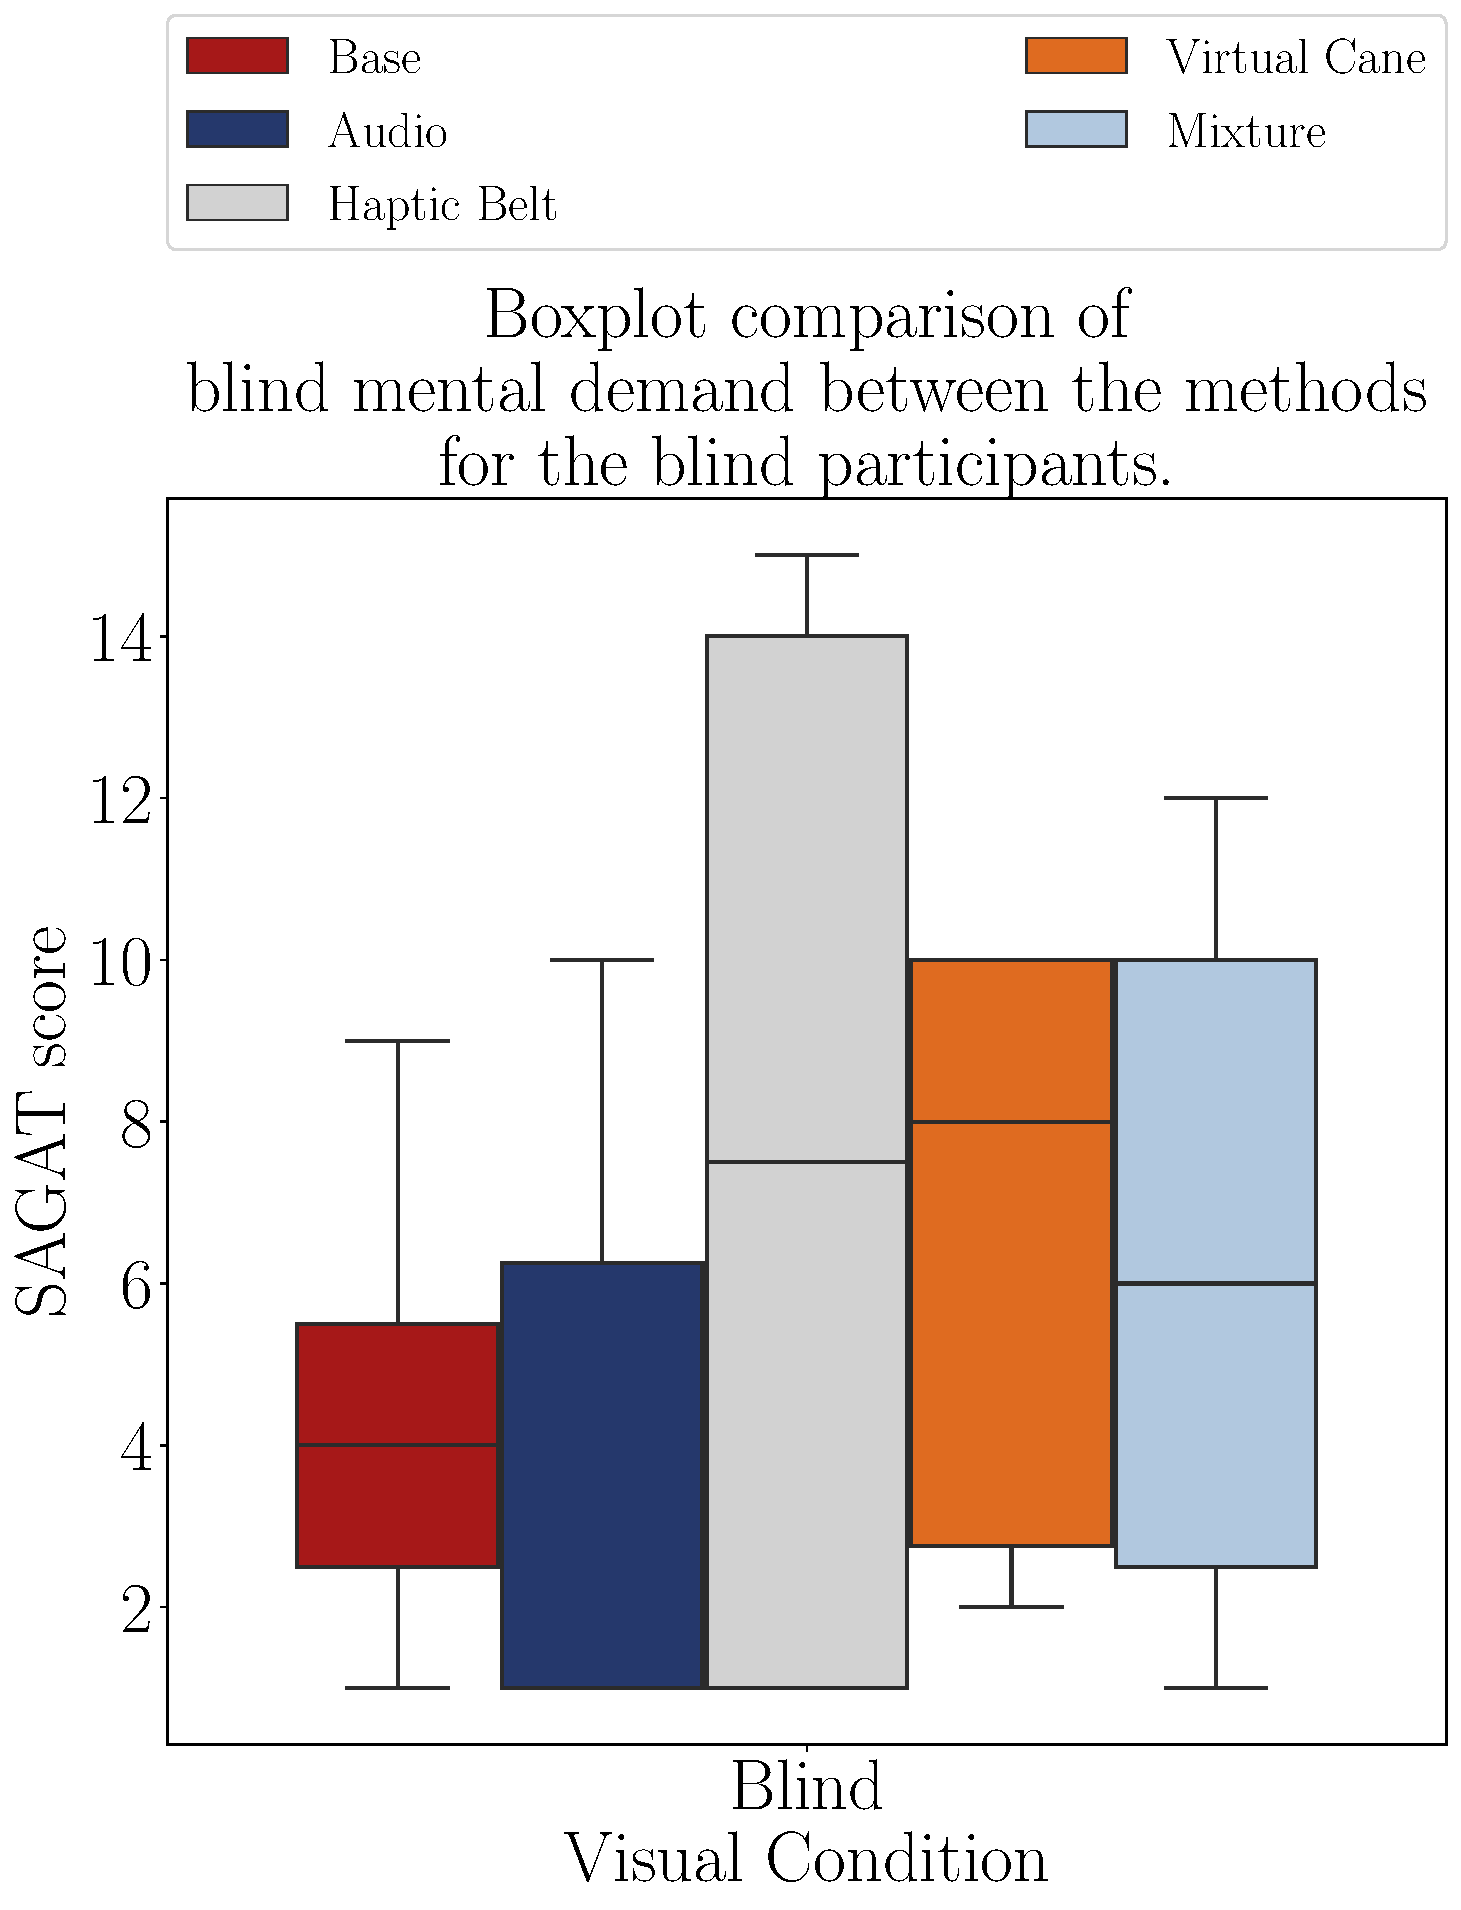
\includegraphics[width = 0.75\linewidth]{3 - Resultados/Figuras/boxplot_md_blind_scene.pdf}
    \caption{Boxplot of the mental demand of the blind participants grouped by the methods.}
    \label{fig:boxplot_md_blind_scene}
\end{figure}    
\begin{figure}[!htb]
    \centering
    %\vspace{3ex}
    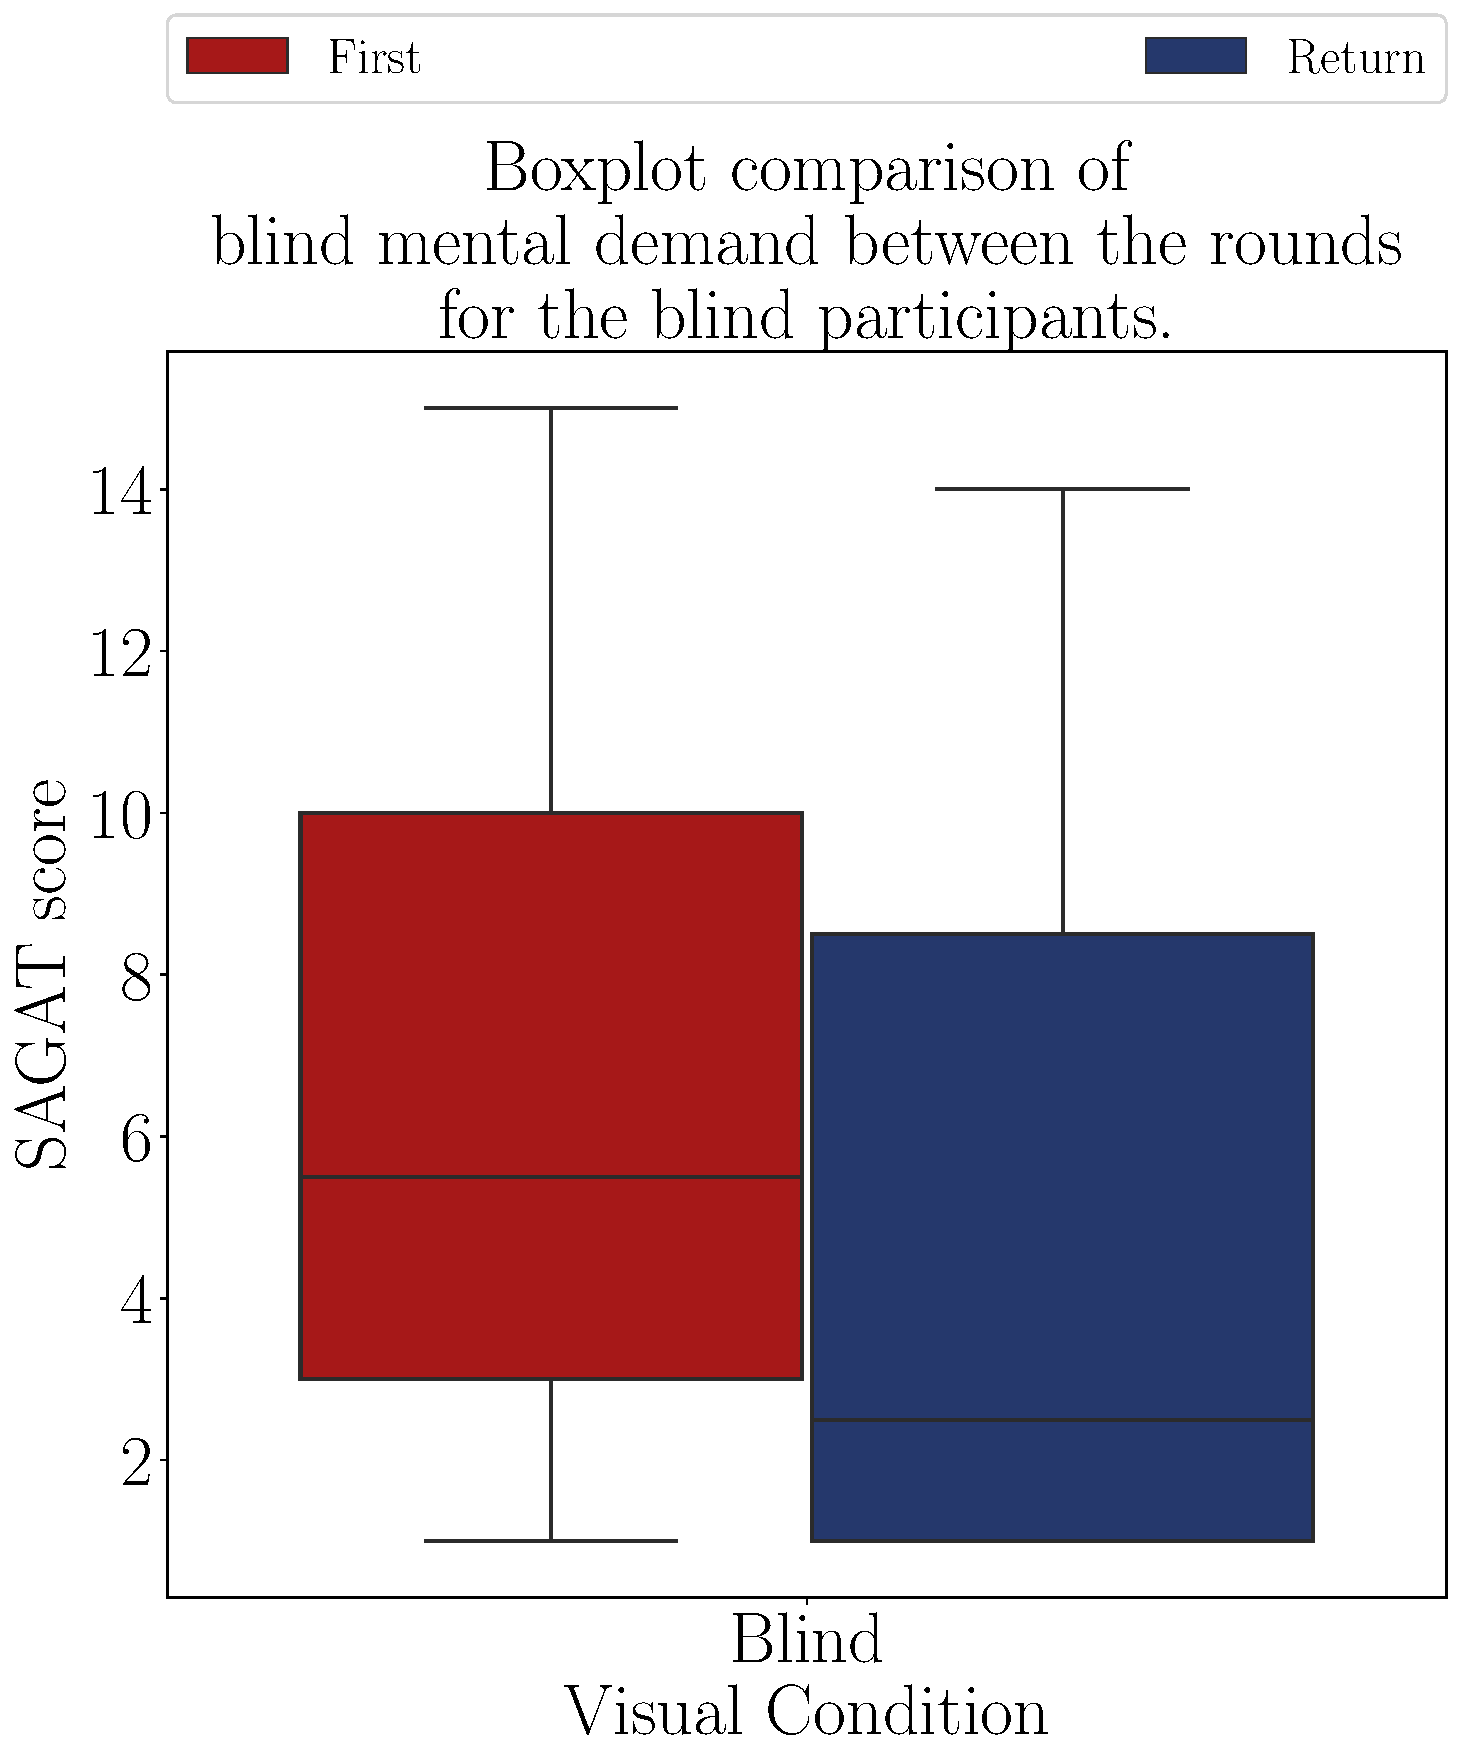
\includegraphics[width = 0.75\linewidth]{3 - Resultados/Figuras/boxplot_md_blind_rounds.pdf}
    \caption{Boxplot of the mental demand of the blind participants grouped by the rounds.}
    \label{fig:boxplot_md_blind_rounds}
\end{figure}

The results of ANOVA are presented in Table \ref{tab:blocanova_md_avg_two_way_blind}. A p-value of 0.05 is commonly adopted as a threshold to confirm the hypothesis. According to this criterion, neither method or round have a significant influence on the mental demand.


\begin{table}[!htb]
\centering
\caption{ANOVA p-value for mental demand -- blind participants}
\label{tab:blocanova_md_avg_two_way_blind}
\begin{tabular}{ll}
\toprule
          Source & P-Value \\
\midrule
    \    Methods &   0.170 \\
     \    Rounds &   0.075 \\
\    Interaction &   0.993 \\
\bottomrule
\end{tabular}
\end{table}



\paragraph*{Analysis of the NASA-TLX score}\mbox{}\\

Figure \ref{fig:boxplot_nasa_blind_scene} presents the boxplot with the NASA-TLX global score grouped by the methods. Similar to what happened for the "mental demand", it is possible to split the methods into two different groups: base and audio, which require a lower level of workload, and another group, which requires a higher level. Figure \ref{fig:boxplot_nasa_blind_rounds} presents a boxplot with the NASA-TLX global score grouped by the rounds, showing that the two groups are still different. 

\begin{figure}[!htb]
    \centering
    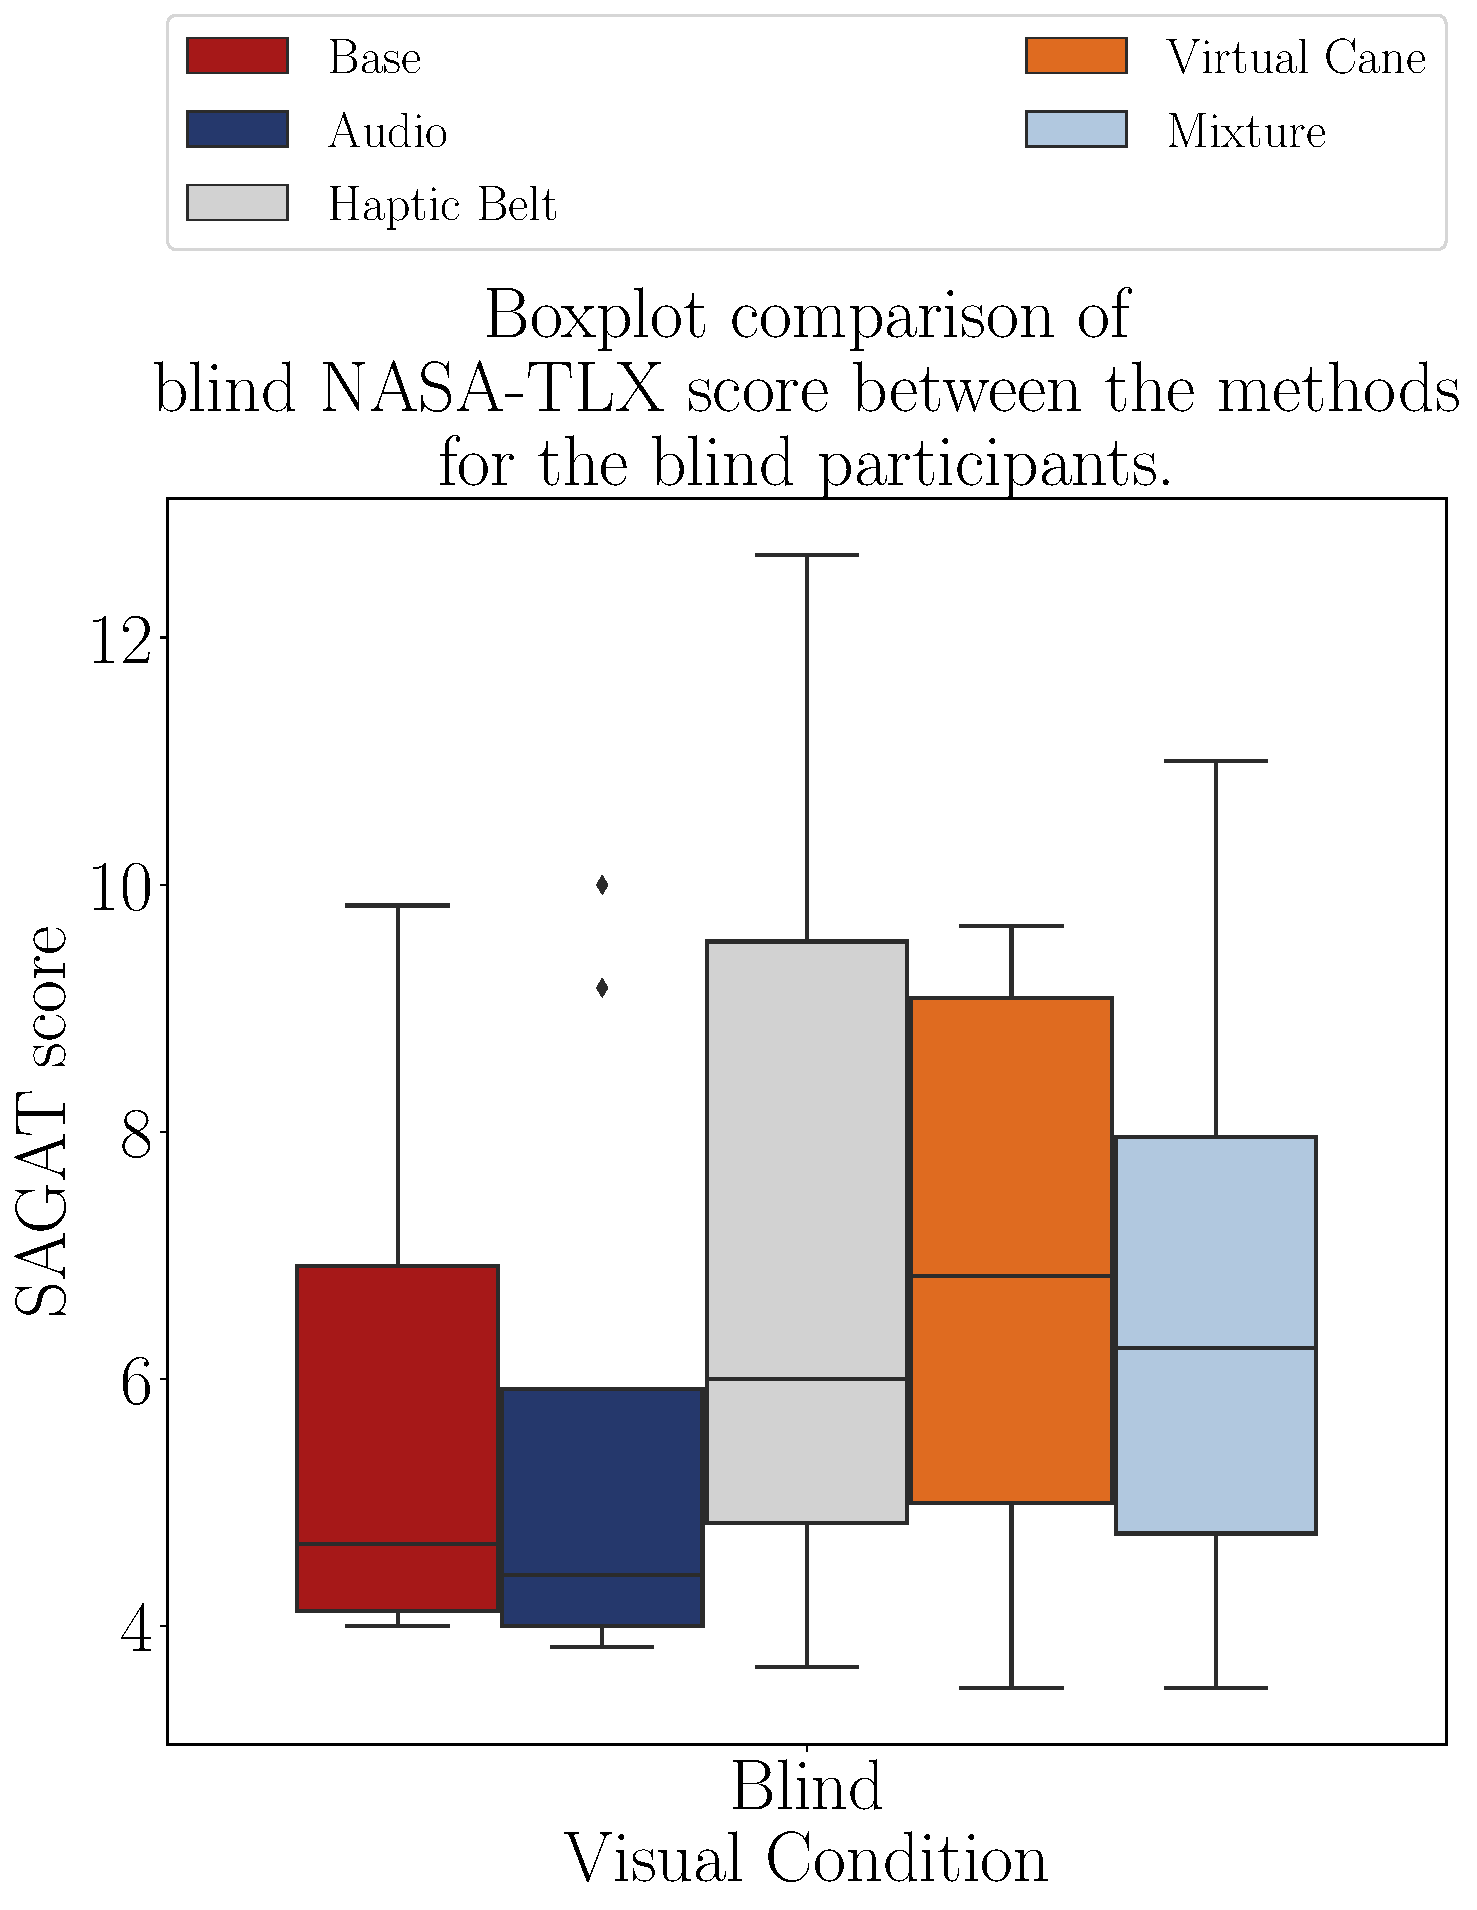
\includegraphics[width = 0.75\linewidth]{3 - Resultados/Figuras/boxplot_nasa_blind_scene.pdf}
    \caption{Boxplot of the mental demand of the blind participants grouped by the methods.}
    \label{fig:boxplot_nasa_blind_scene}
\end{figure}    
\begin{figure}[!htb]
    \centering
    %\vspace{3ex}
    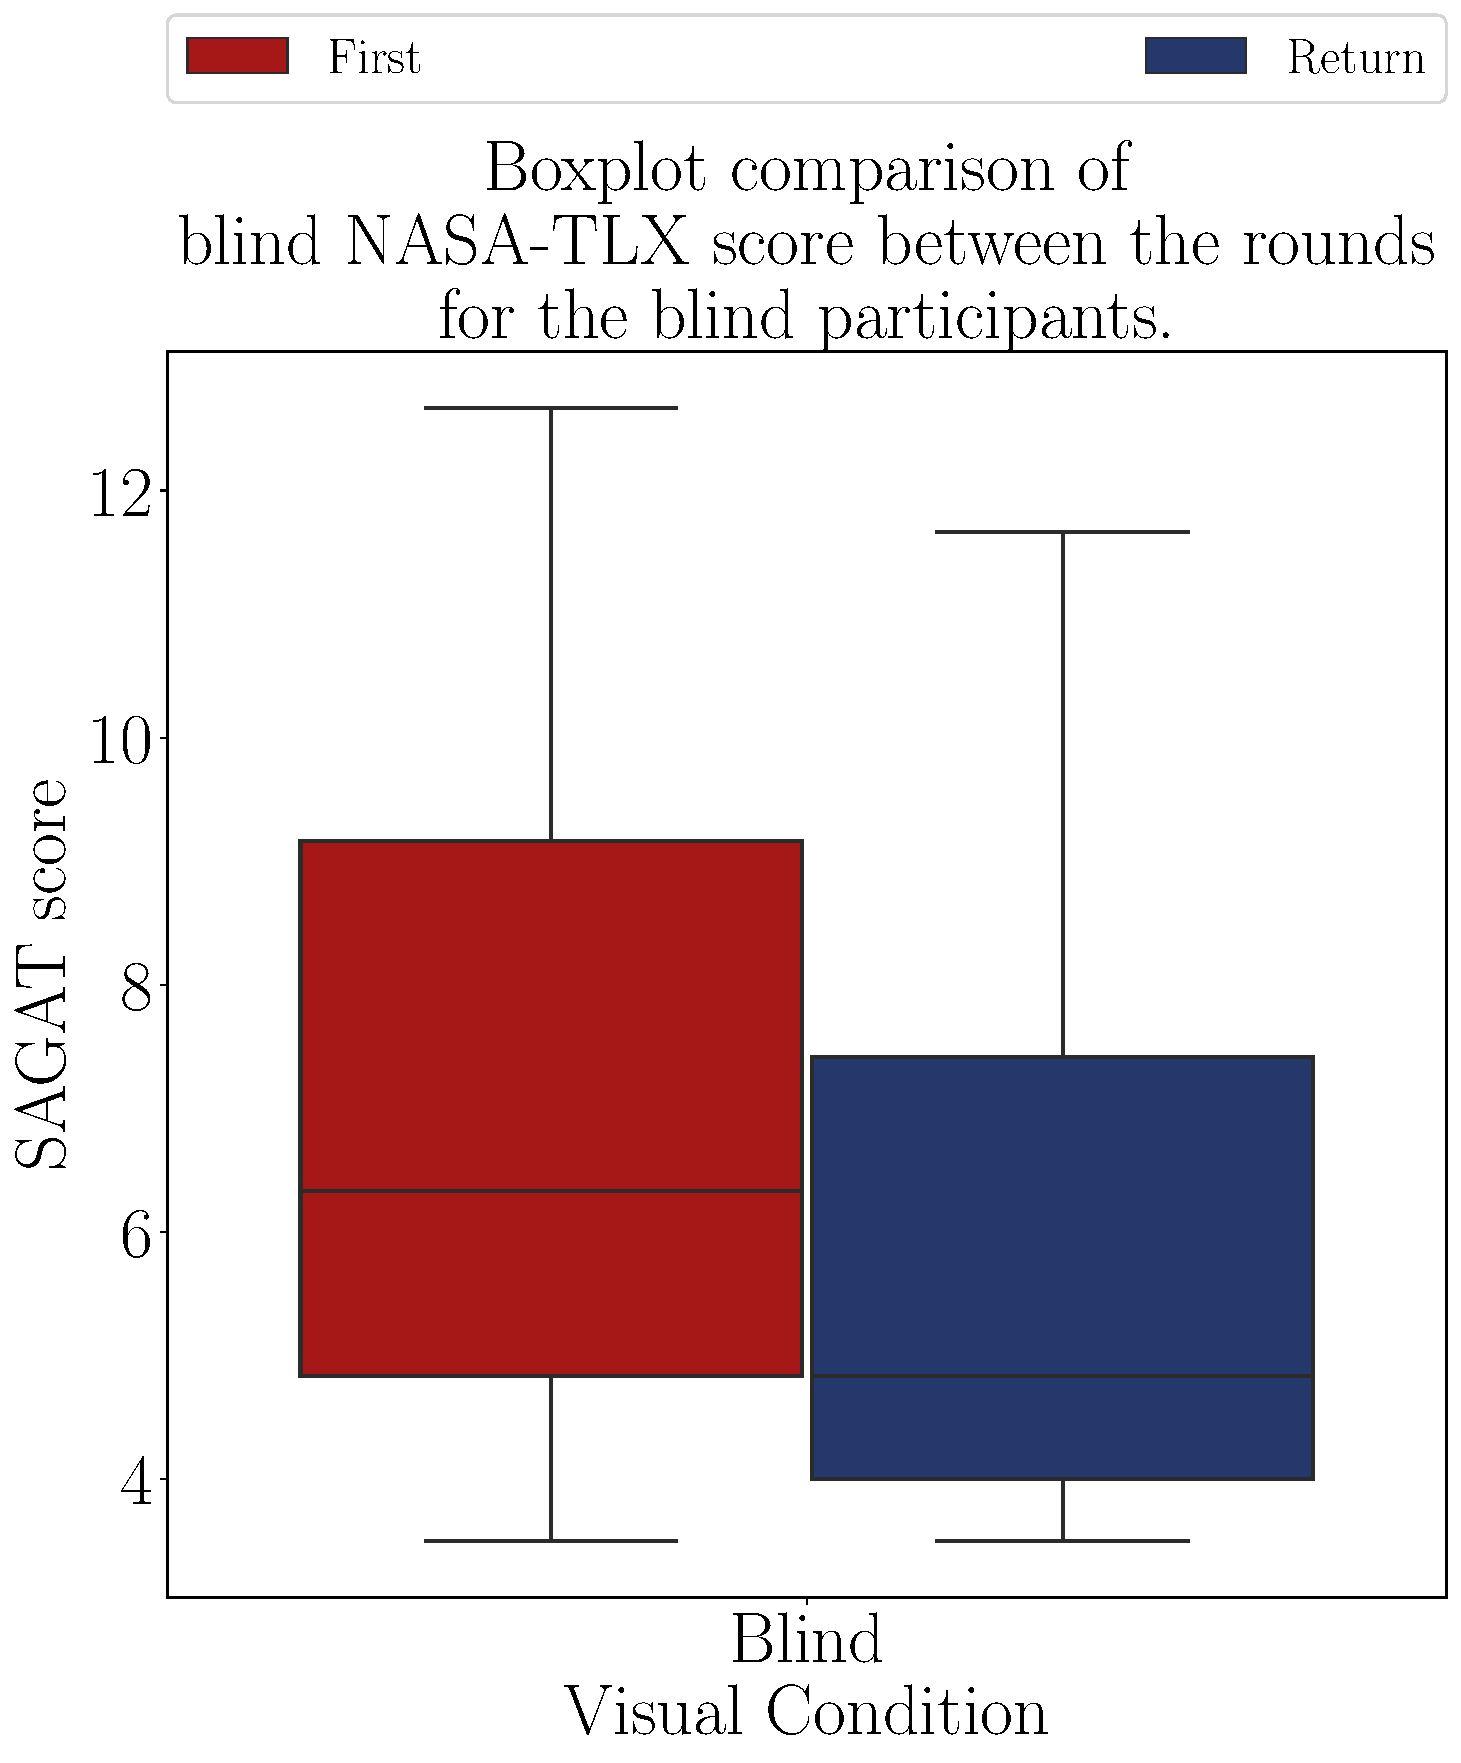
\includegraphics[width = 0.75\linewidth]{3 - Resultados/Figuras/boxplot_nasa_blind_rounds.pdf}
    \caption{Boxplot of the mental demand of the blind participants grouped by the rounds.}
    \label{fig:boxplot_nasa_blind_rounds}
\end{figure}

The sample residuals are not homogeneous meaning that the participants have different variability among them and that impacts the ANOVA.

Table \ref{tab:blocanova_nasa_avg_two_way_blind} brings the p-value resulting from ANOVA. In this case, both the methods and the rounds were appointed as significant variables that influence the mean value of the NASA-TLX global score. 


\begin{table}[!htb]
\centering
\caption{Anova p-value for the NASA-TLX score -- blinded users.}
\label{tab:blocanova_nasa_avg_two_way_blind}
\begin{tabular}{lrrrrl}
\toprule
          Source & P-Value \\
\midrule
    \    Methods & 0.029** \\
     \    Rounds & 0.022** \\
\    Interaction &   0.814 \\
\bottomrule
\end{tabular}
\end{table}



Finally a pairwise Fisher LSD test comparing each pair of guidance methods. The results show that only audio is similar to the base. All the other methods are different from each other.
\subsubsection{Adapted SAGAT}
\label{subsubsec:results_adapted_sagat_1}

For each question of the SAGAT questionnaire, the participant could score 1 point or a fraction of it. The closer to the value 1, higher is the situation awareness of the user. 

Figure \ref{fig:boxplot_sagat_blind_scene} brings the boxplot of the SAGAT score grouped by the guidance methods. It shows that the methods can be divided into two groups. The first one is composed of base, haptic belt and the mixture. This group received scores higher than the second group, composed of audio and virtual cane. Figure \ref{fig:boxplot_sagat_blind_rounds} shows the boxplot of the data grouped by round and confirms the general improvement of situation awareness from the first to the return round. 

\begin{figure}[!htb]
    \centering
    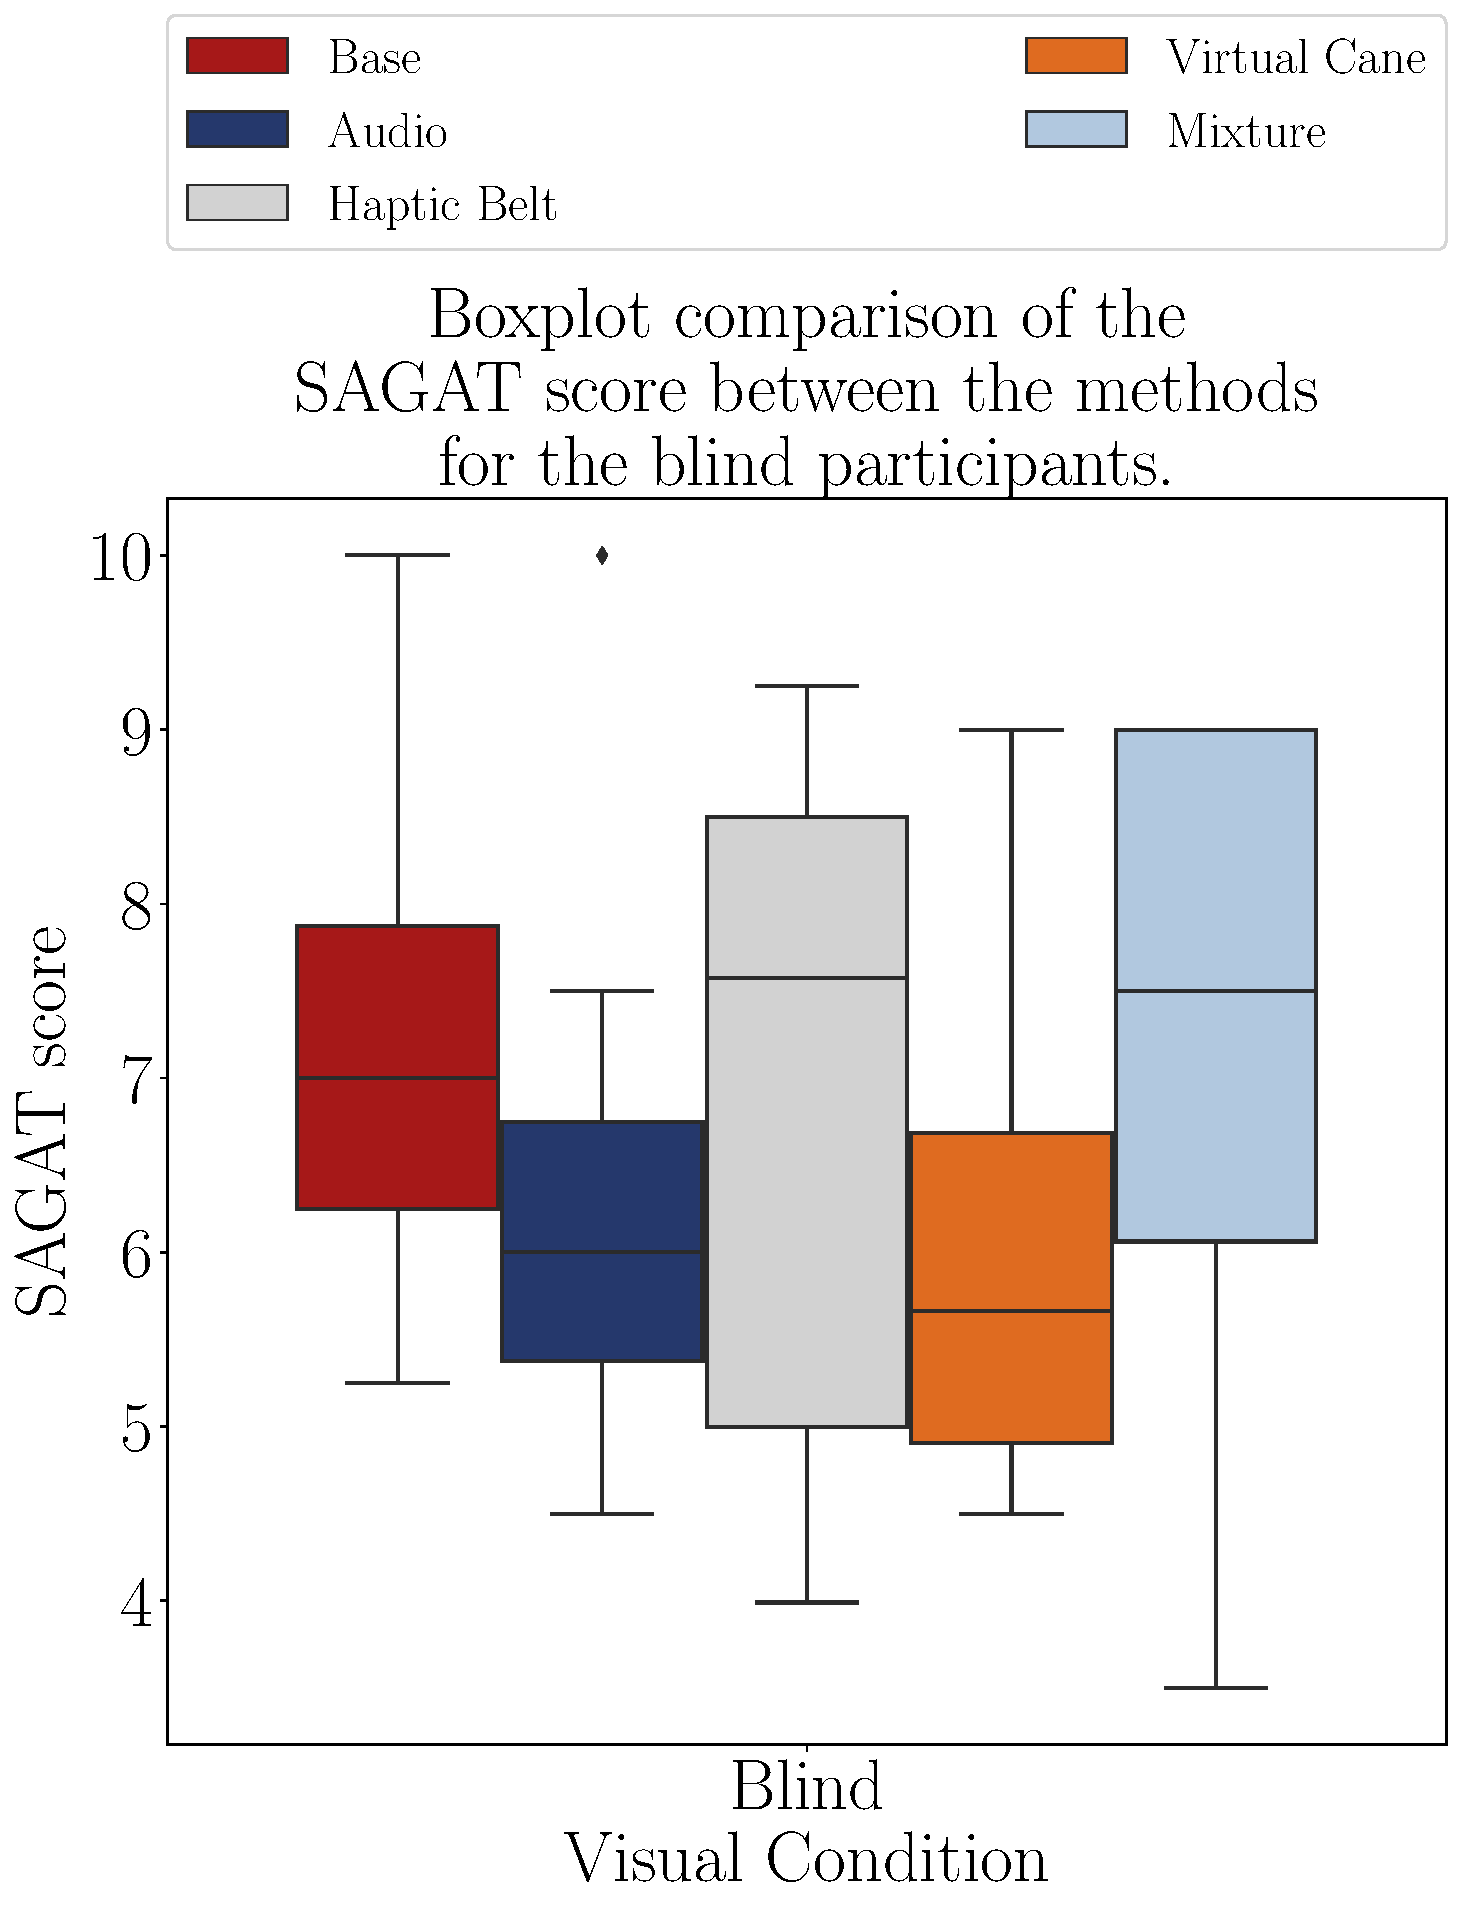
\includegraphics[width = 0.75\linewidth]{3 - Resultados/Figuras/boxplot_sagat_blind_scene.pdf}
    \caption{Boxplot of the SAGAT score of the blind participants grouped by the methods.}
    \label{fig:boxplot_sagat_blind_scene}
\end{figure}

\begin{figure}[!htb]
    \centering
    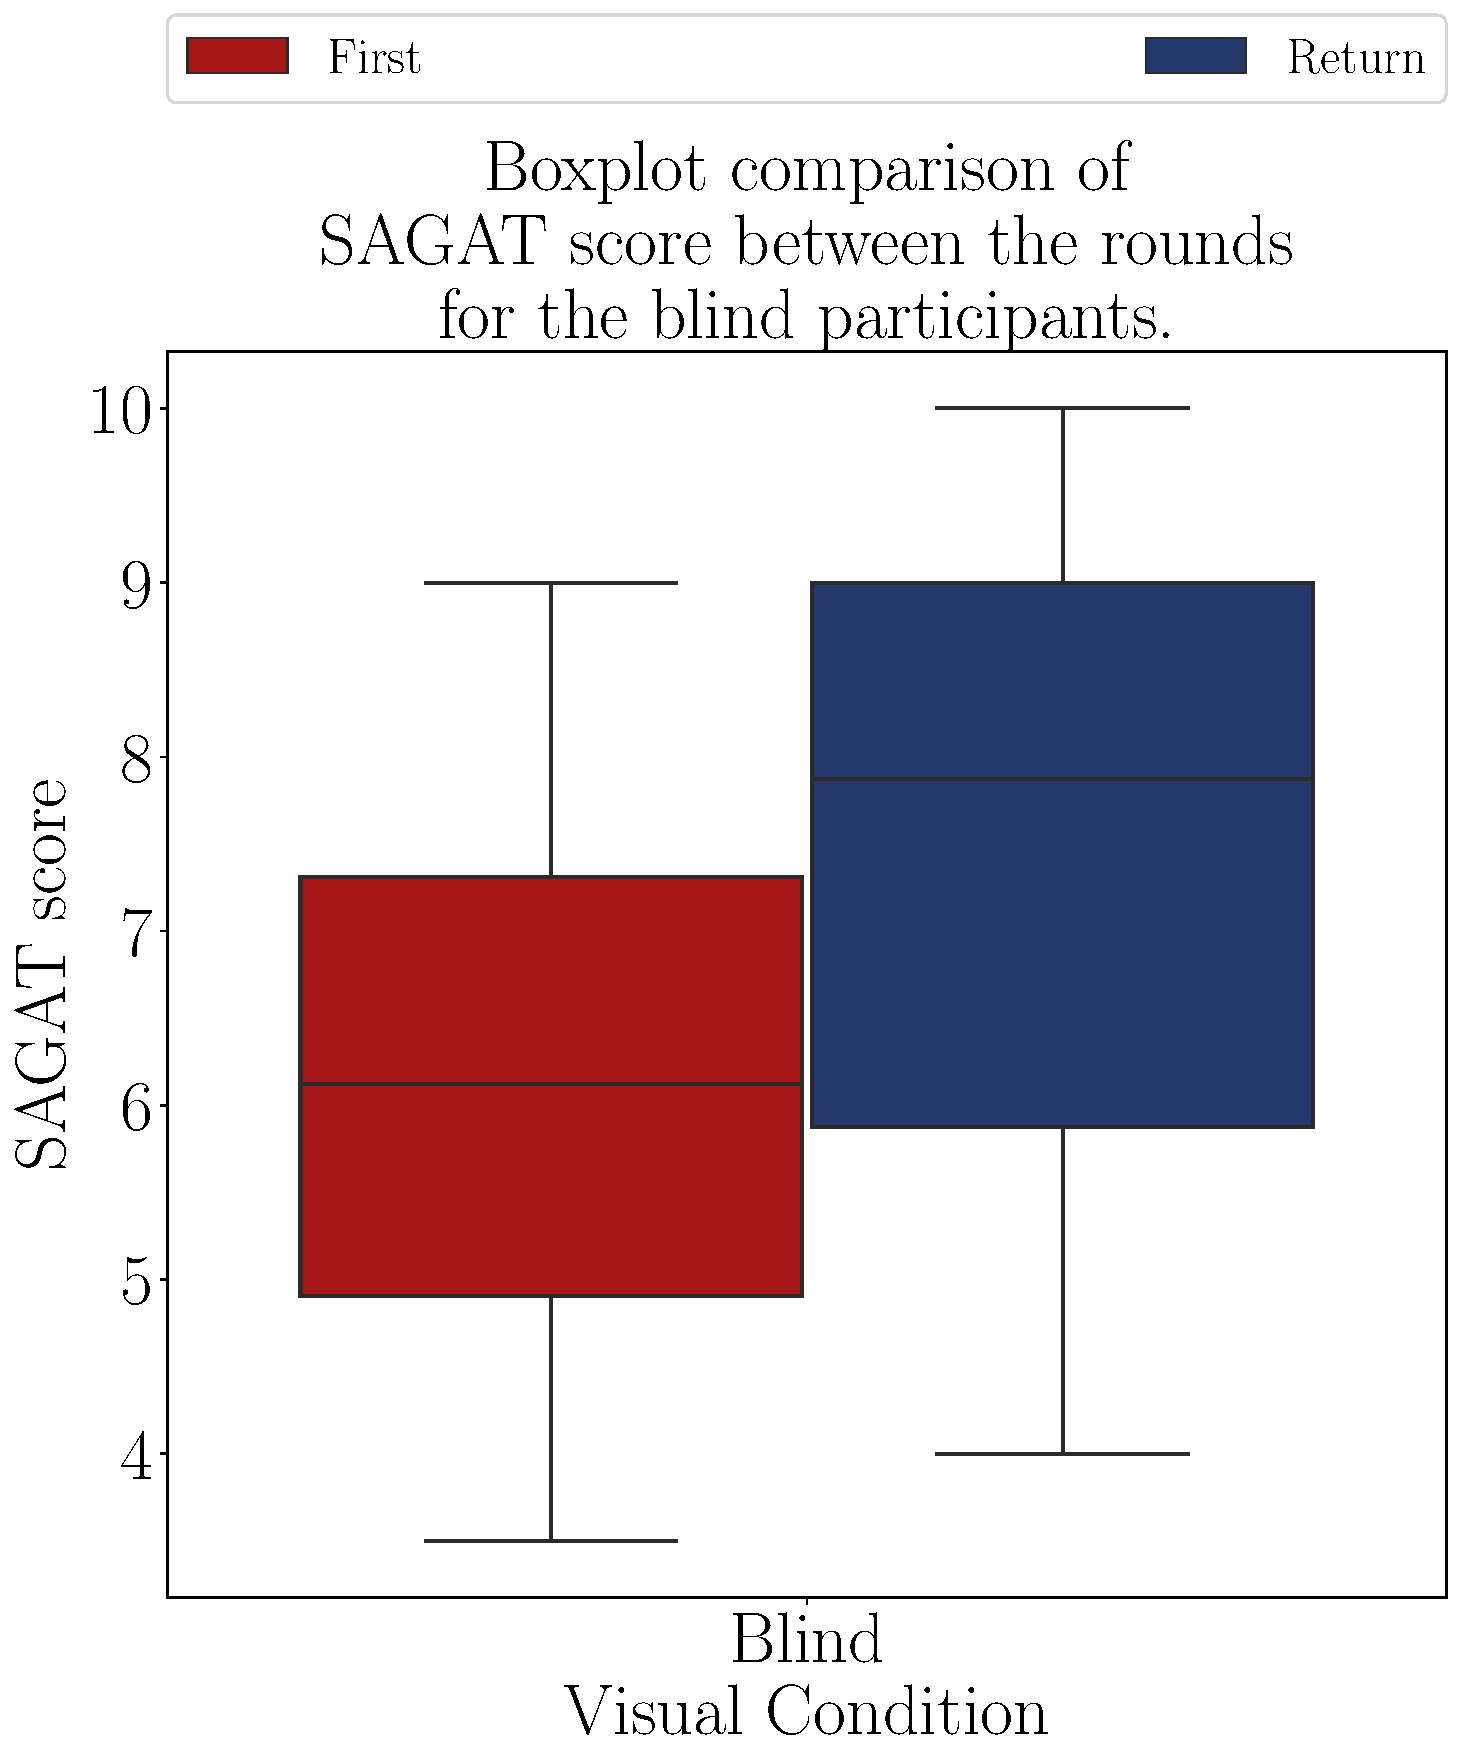
\includegraphics[width = 0.75\linewidth]{3 - Resultados/Figuras/boxplot_sagat_blind_rounds.pdf}
    \caption{Boxplot of the SAGAT score of the blind participants grouped by the rounds.}
    \label{fig:boxplot_sagat_blind_rounds}
\end{figure}

Table \ref{tab:blocanova_sagat_avg_two_way_blind} shows the ANOVA test p-value of the SAGAT score. It indicates that the round is a significant variable that influences the value of the SAGAT score. The same cannot be said for the method, which has no significant influence.


\begin{table}[!htb]
\centering
\caption{Anova p-value for the SAGAT score on each method for blinded users.}
\label{tab:blocanova_sagat_avg_two_way_blind}
\begin{tabular}{lrrrrr}
\toprule
          Source & P-Value \\
\midrule
    \    Methods &   0.277 \\
     \    Rounds & 0.002** \\
\    Interaction &   0.834 \\
\bottomrule
\end{tabular}
\end{table}


\subsubsection{Guidance method's questionnaire.}
\label{subsubsec:results_questionnaires}

The data from the questionnaire for evaluating the user experience with each guidance method is also analysed. The higher the score, the more satisfied the user is with the method. It is essential to observe that this analysis does not include the base method as the questions are specific about each method and the base may vary among the participants. Also, there is no distinction between first and return rounds. Each questionnaire is answered only once for each method.
Figure \ref{fig:boxplot_quest_blind_scene} brings the questionnaire boxplot, which clearly shows the difference between two groups: haptic belt and virtual cane, and audio and mixture. 

\begin{figure}[!htb]
    \centering
    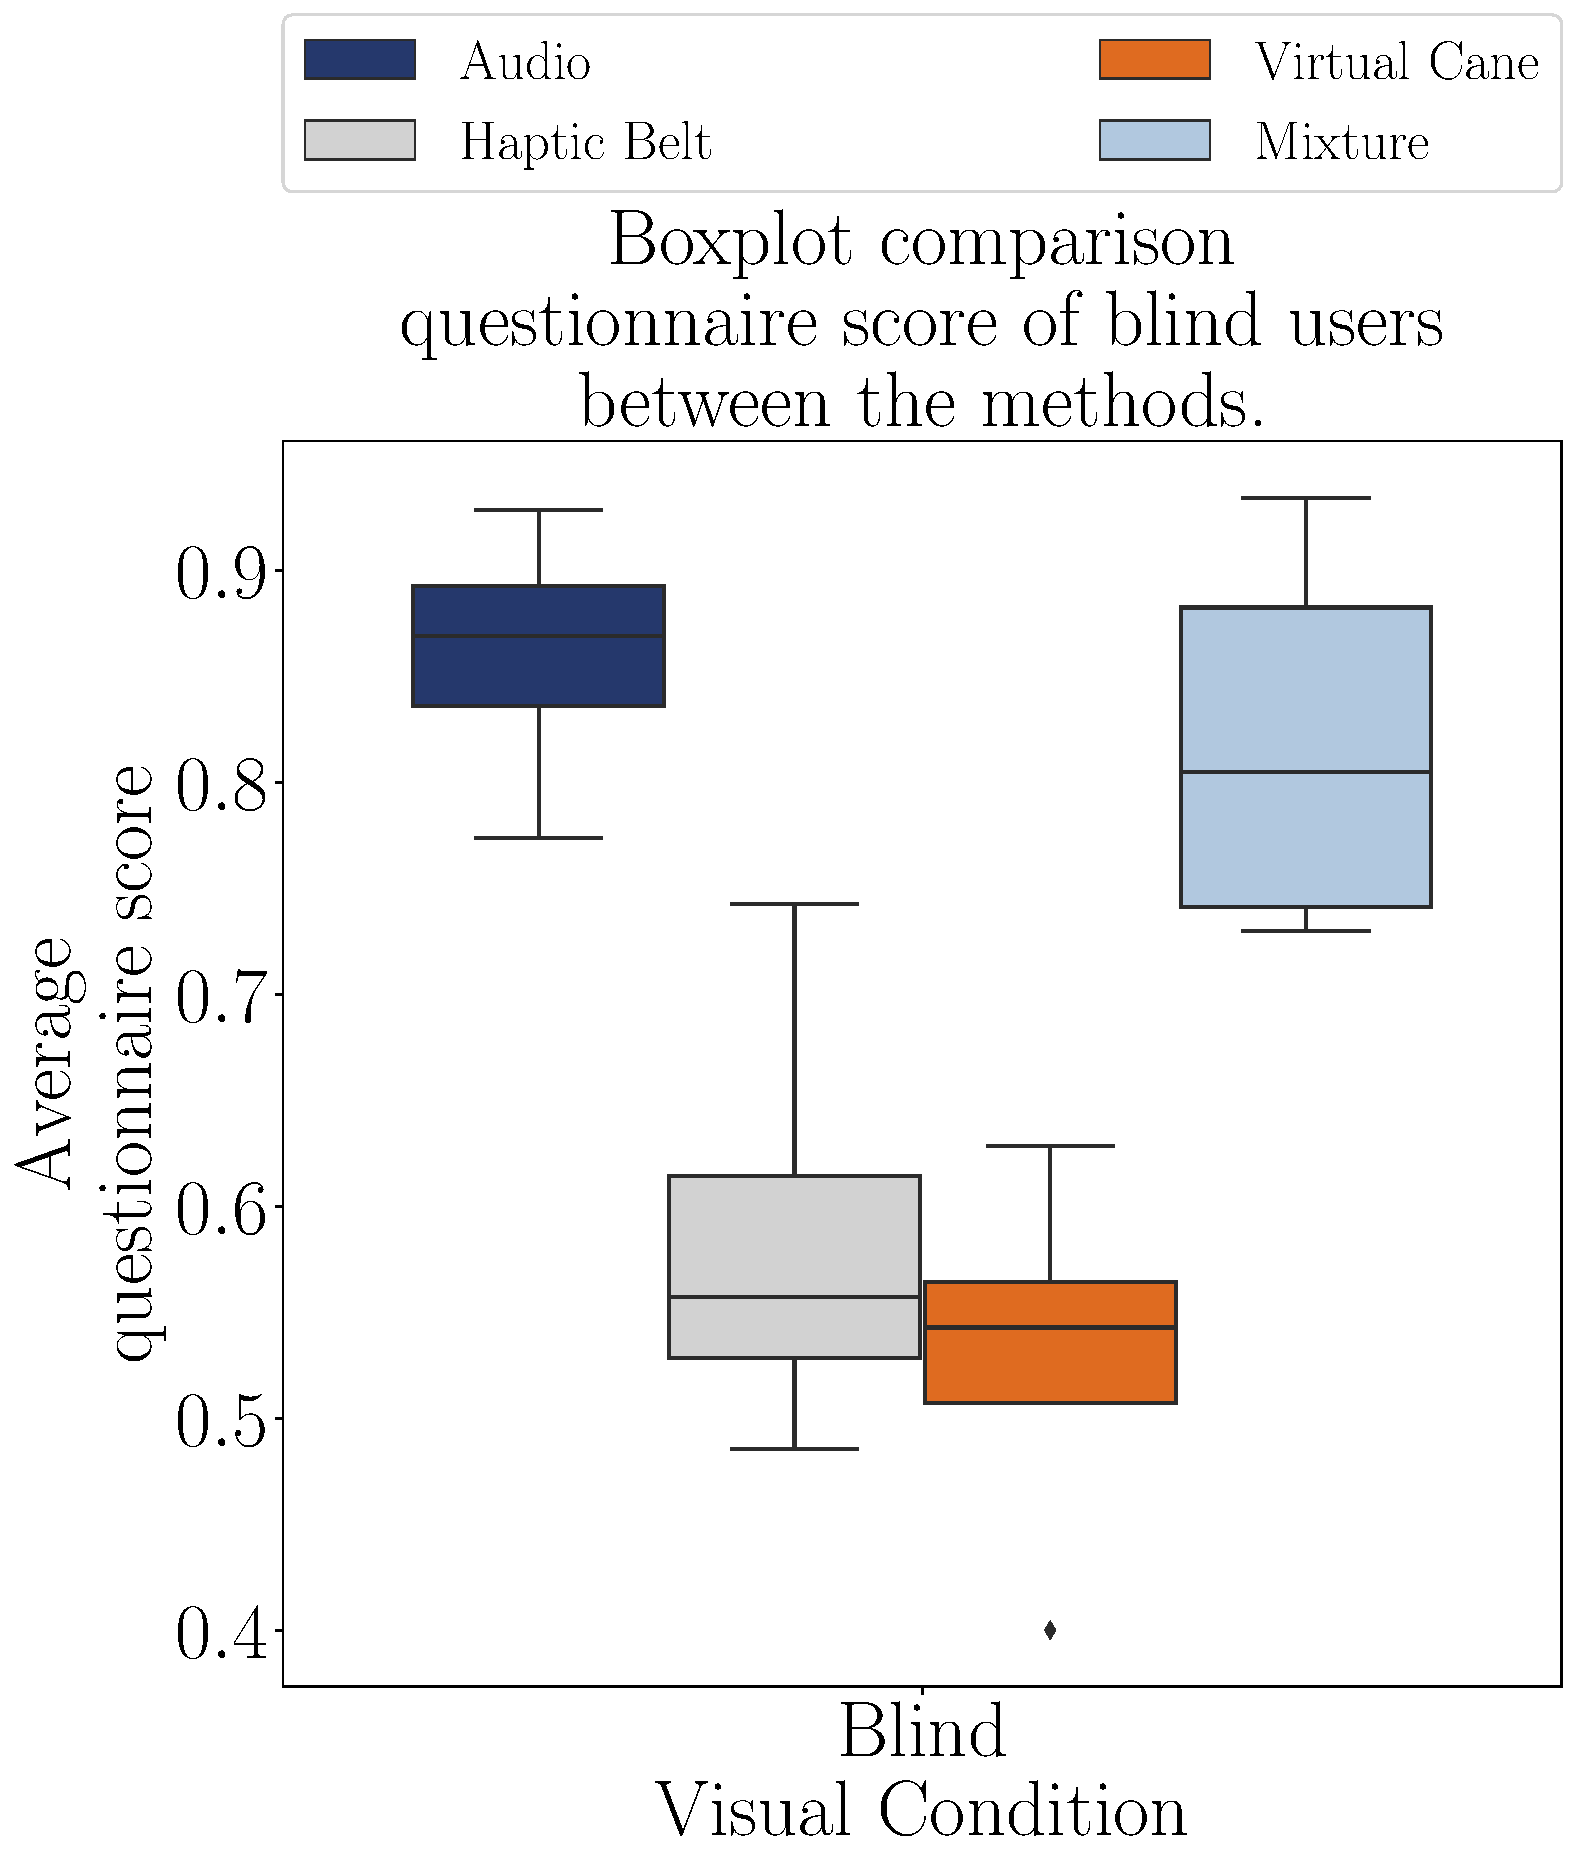
\includegraphics[width = 0.75\linewidth]{3 - Resultados/Figuras/boxplot_questionnaire_scene_blind.pdf}
    \caption{Boxplot of the questionaire score of the blind participants grouped by the methods.}
    \label{fig:boxplot_quest_blind_scene}
\end{figure}

The results of ANOVA are presented in Table  \ref{tab:blocanova_questionnaire_blind} and it shows that the method, with a p-value of 0.001, is indeed a significant variable that affects the user's satisfaction.


\begin{table}[!htb]
\centering
\caption{Anova p-value for the questionnaire score -- blinded users.}
\label{tab:blocanova_questionnaire_blind}
\begin{tabular}{lrrrrr}
\toprule
Source & P-Value \\
\midrule
Method & 0.001** \\
\bottomrule
\end{tabular}
\end{table}



In order to complement the ANOVA analysis, the pairwise comparison of the methods obtained from the Fisher LSD shows that audio and mixture are equivalent from the perspective of user satisfaction. All the other comparisons indicate there is a difference between the methods.

Additional to the scores, the participants also expressed their dissatisfaction with the answers to the open questions of the questionnaire, where they commented that the haptic belt and the virtual cane are confusing, are not precise enough, and are very different from what they are used to.

%\subsection{Physiological data}

%During the experiment, data from two physiological sensors were captured: ECG and GSR. As commonly found in the literature, these data are used to assess mental workload. The corresponding analysis is presented in this section.

\subsubsection{Electrocardiogram (ECG) data}
\label{subsubsec:results_ecg_1}

After the experiment, the ECG signal processing is organized in the following steps: 

\begin{itemize}
    \item Filtering and removing outliers. Since the participants moved during the whole experience, the sensors also captured some noise data.
    \item Normalization between -1 and 1;
    \item Peak detection and evaluation – if the results were not of good quality, the peak detection method's parameters were adjusted to improve it; 
    \item Calculation of BPM using Kubius HRV Standard;
    \item Calculation of SDNN using Kubius HRV Standard.
\end{itemize}

At the beginning of each experiment, a baseline was collected to establish a comparison between the relaxed state of the participant and the scenes' induced state. However, the results were not consistent.  During the experiment, it was expected that the heart rate would increase compared to the baseline because the participants were at rest. However, for most of the participants, it decreased, indicating a systematic problem may have occurred. Due to this fact, the analysis is based only on absolute values.

\paragraph*{Analysis of the heartbeat frequency (BPM)}\mbox{}\\

Figures \ref{fig:boxplot_ecg_bpm_blind_scene} and \ref{fig:boxplot_ecg_bpm_blind_rounds} brings the corresponding boxplot, grouped by method and round. In both cases, it is not possible to observe significant differences among the methods or rounds.

\begin{figure}[!htb]
    \centering
    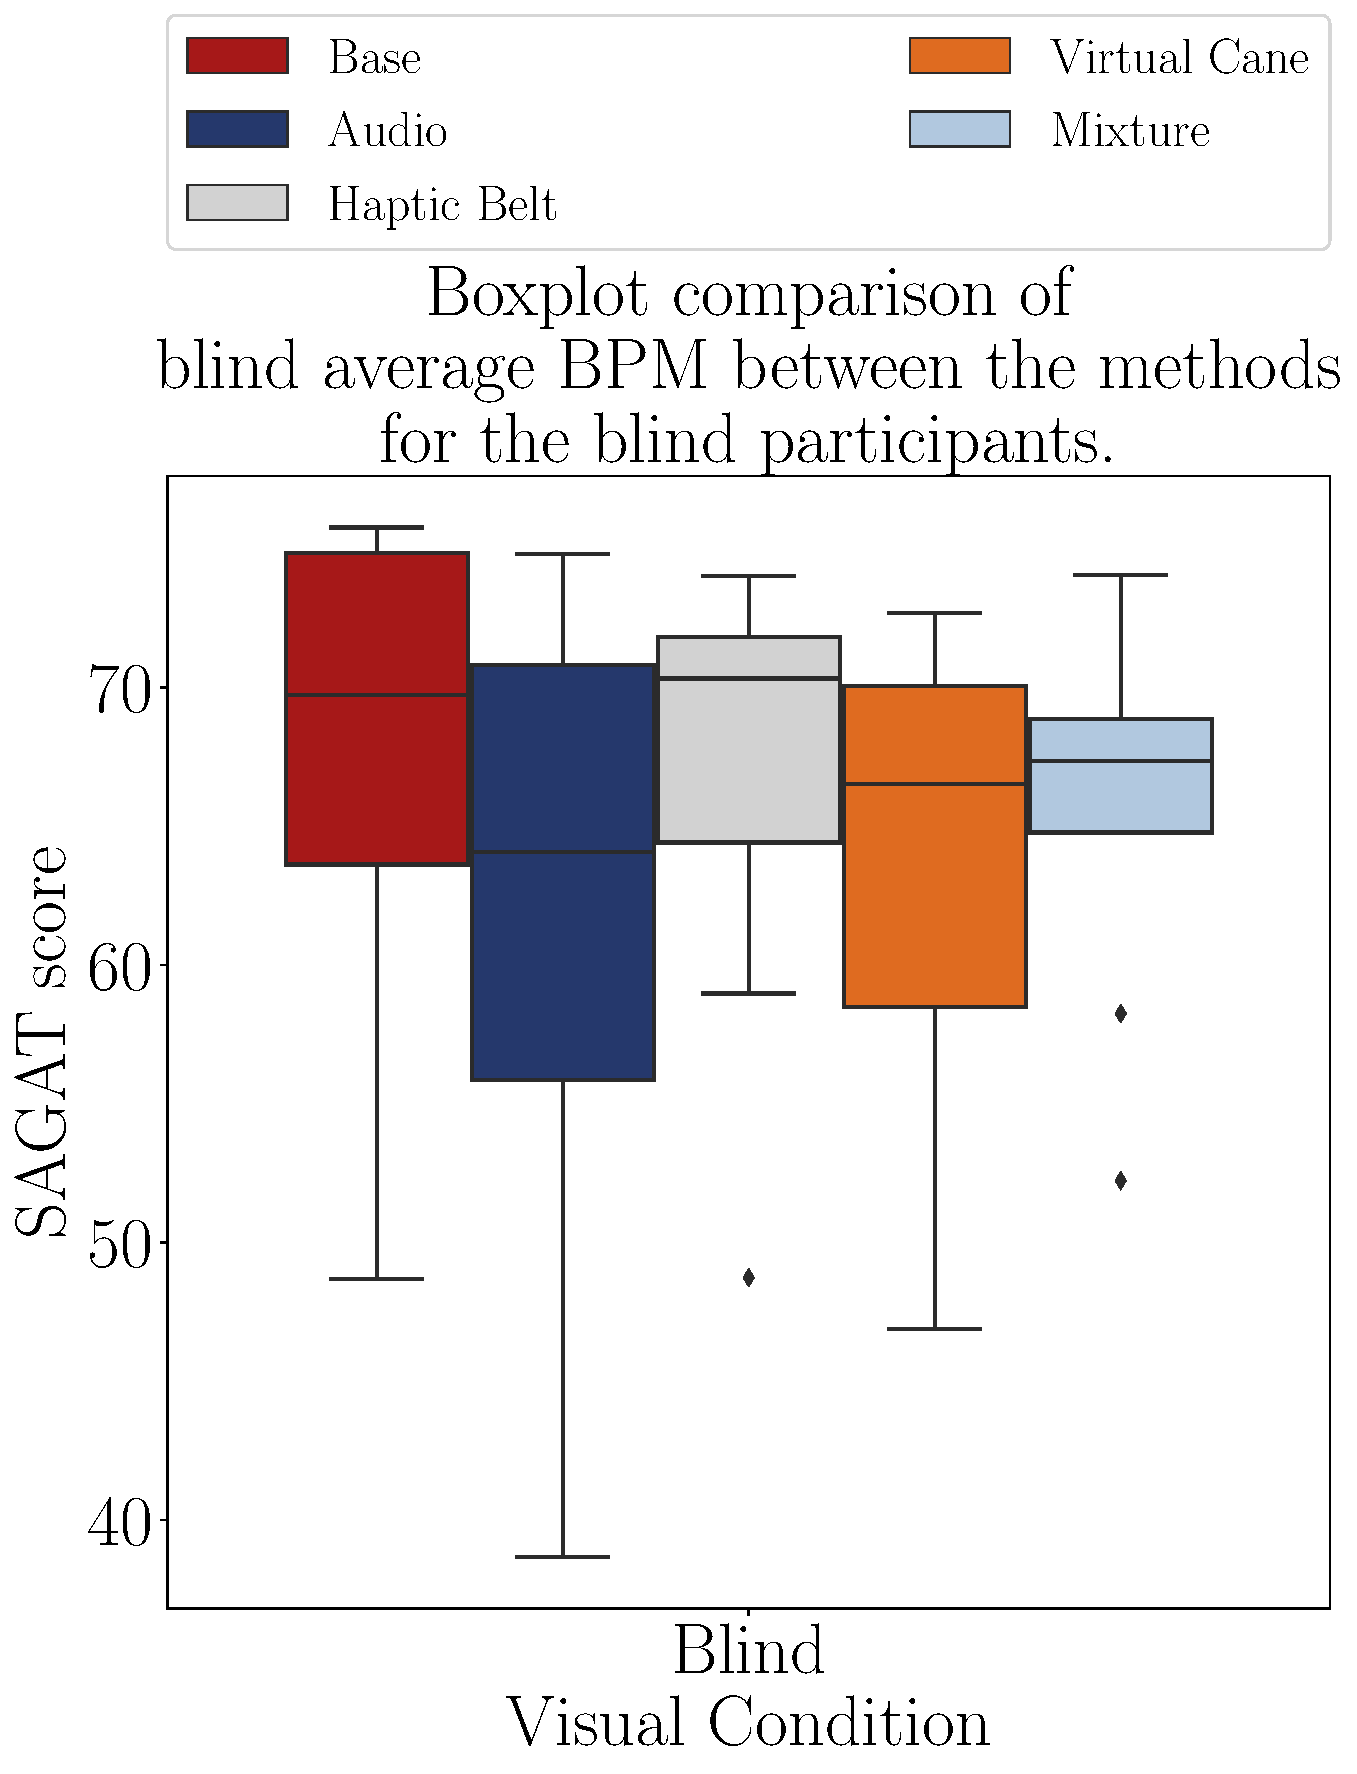
\includegraphics[width = 0.75\linewidth]{3 - Resultados/Figuras/boxplot_ecg_bpm_blind_scene.pdf}
    \caption{Boxplot of the BPM of the blind participants grouped by the methods.}
    \label{fig:boxplot_ecg_bpm_blind_scene}
\end{figure}

\begin{figure}[!htb]
    \centering
    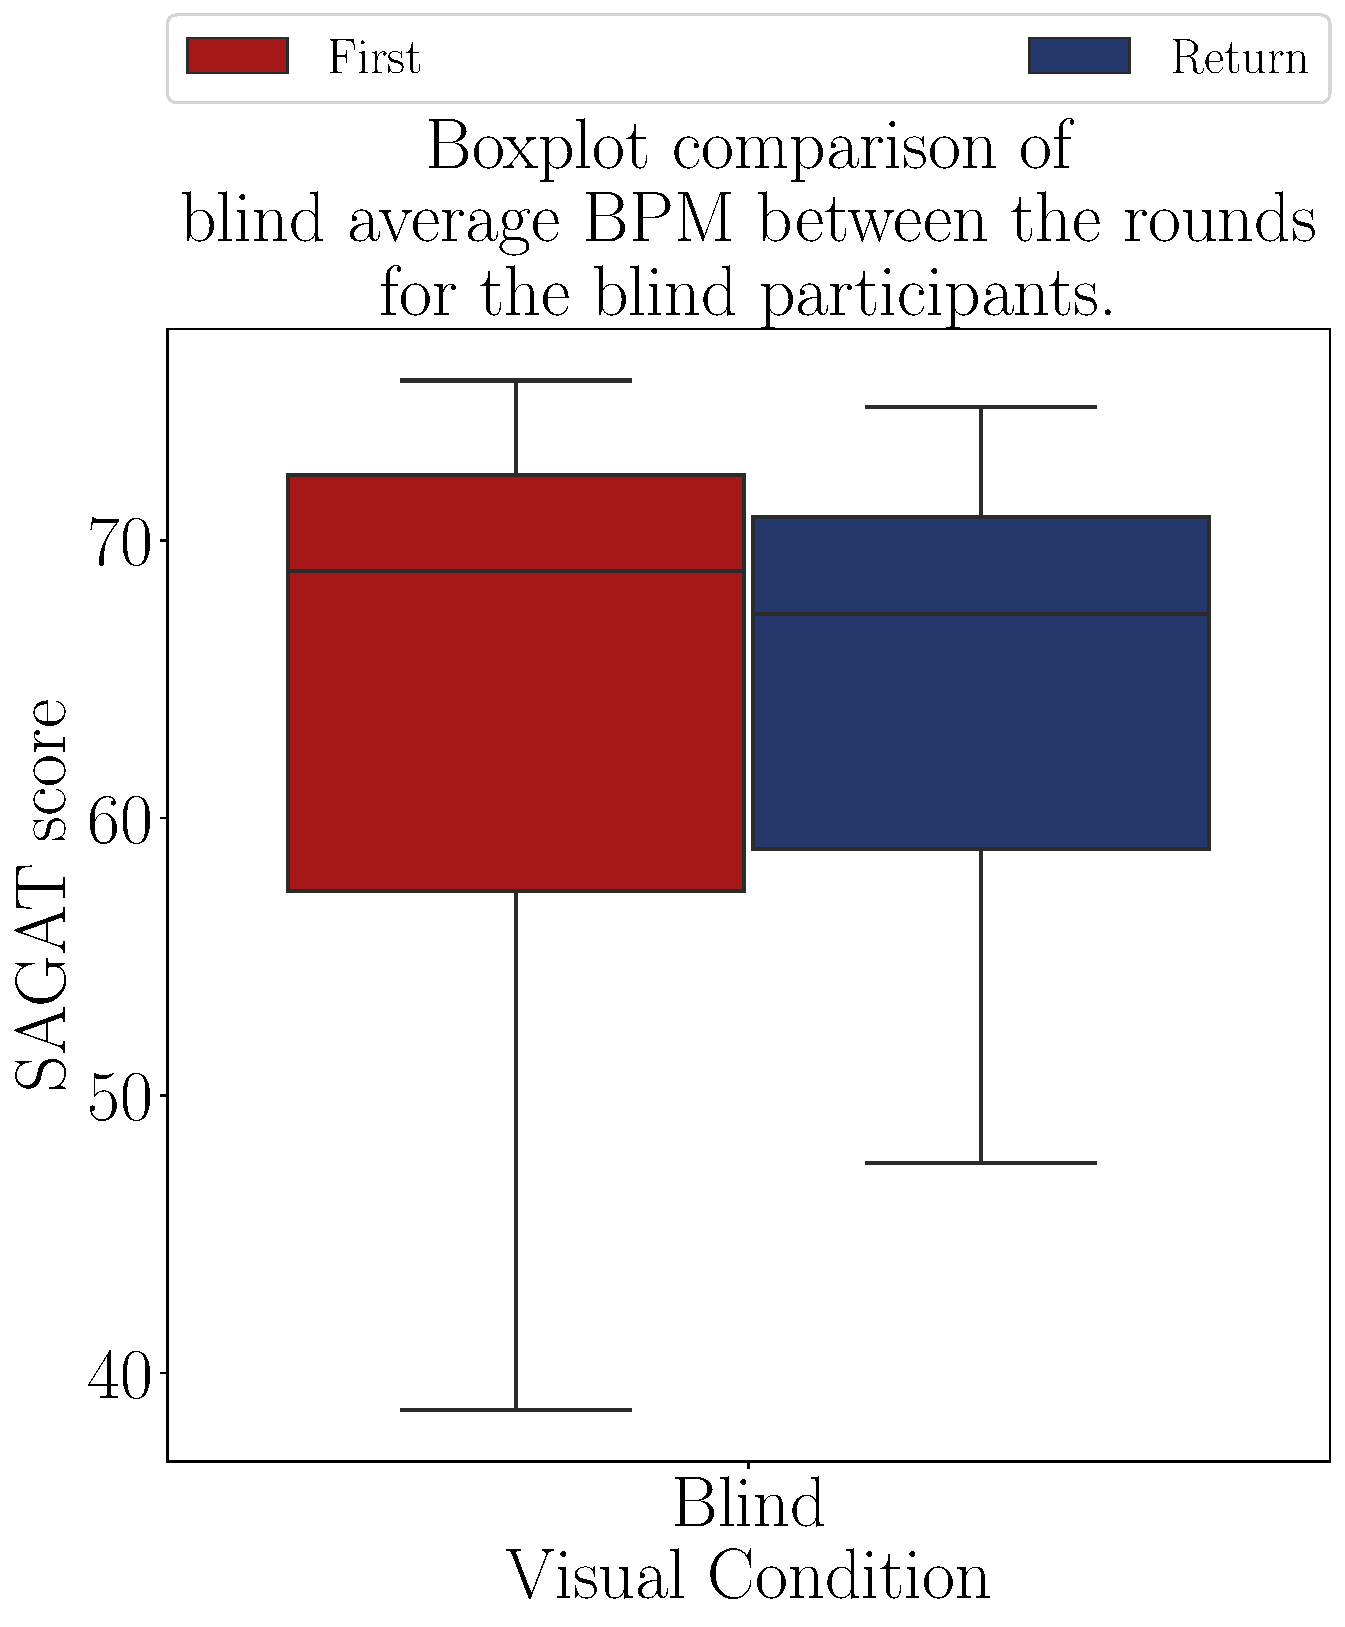
\includegraphics[width = 0.75\linewidth]{3 - Resultados/Figuras/boxplot_ecg_bpm_blind_rounds.pdf}
    \caption{Boxplot of the BPM of the blind participants grouped by the rounds.}
    \label{fig:boxplot_ecg_bpm_blind_rounds}
\end{figure}

The participants do not have a similar variance, which jeopardize the results of ANOVA. Considering this limitation, Table \ref{tab:blocanova_bpm_two_way_blind} brings the p-value obtained by ANOVA, which confirmed the previous analysis, as it does not indicate a significant influence of either the guidance methods or the rounds in the participants' heart rate. 


\begin{table}[!htb]
\centering
\caption{Anova p-value for the BPM -- blinded users.}
\label{tab:blocanova_bpm_two_way_blind}
\begin{tabular}{lrrrrr}
\toprule
          Source & P-Value \\
\midrule
    \    Methods &   0.100 \\
     \    Rounds &   0.371 \\
\    Interaction &   0.894 \\
\bottomrule
\end{tabular}
\end{table}



%%%%%%%%%%%%%%%%%%%%%%%%%%%%%%%%%%%%%%%%%%%%%%%%%%%%%%%%%%%%%%%%%%%%%%%%%%%%
%%%%%%%%%%%%%%%%%%%%%%%%%%%%%%%%%%%%%%%%%%%%%%%%%%%%%%%%%%%%%%%%%%%%%%%%%%%%
%%%%%%%%%%%%%%%%%%%%%%%%%%%%%%%%%%%%%%%%%%%%%%%%%%%%%%%%%%%%%%%%%%%%%%%%%%%%
%%%%%%%%%%%%%%%%%%%%%%%%%%%%%%%%%%%%%%%%%%%%%%%%%%%%%%%%%%%%%%%%%%%%%%%%%%%%

\paragraph*{Analysis of the heartbeat variance (SDNN)}\mbox{}\\

Figure \ref{fig:boxplot_ecg_sdnn_blind_scene} and Figure \ref{fig:boxplot_ecg_sdnn_blind_rounds} bring the SDNN barplot grouped by the methods and the rounds. There is a slight tendency among the participants to increase the heartbeat in the return round.

\begin{figure}[!htb]
    \centering
    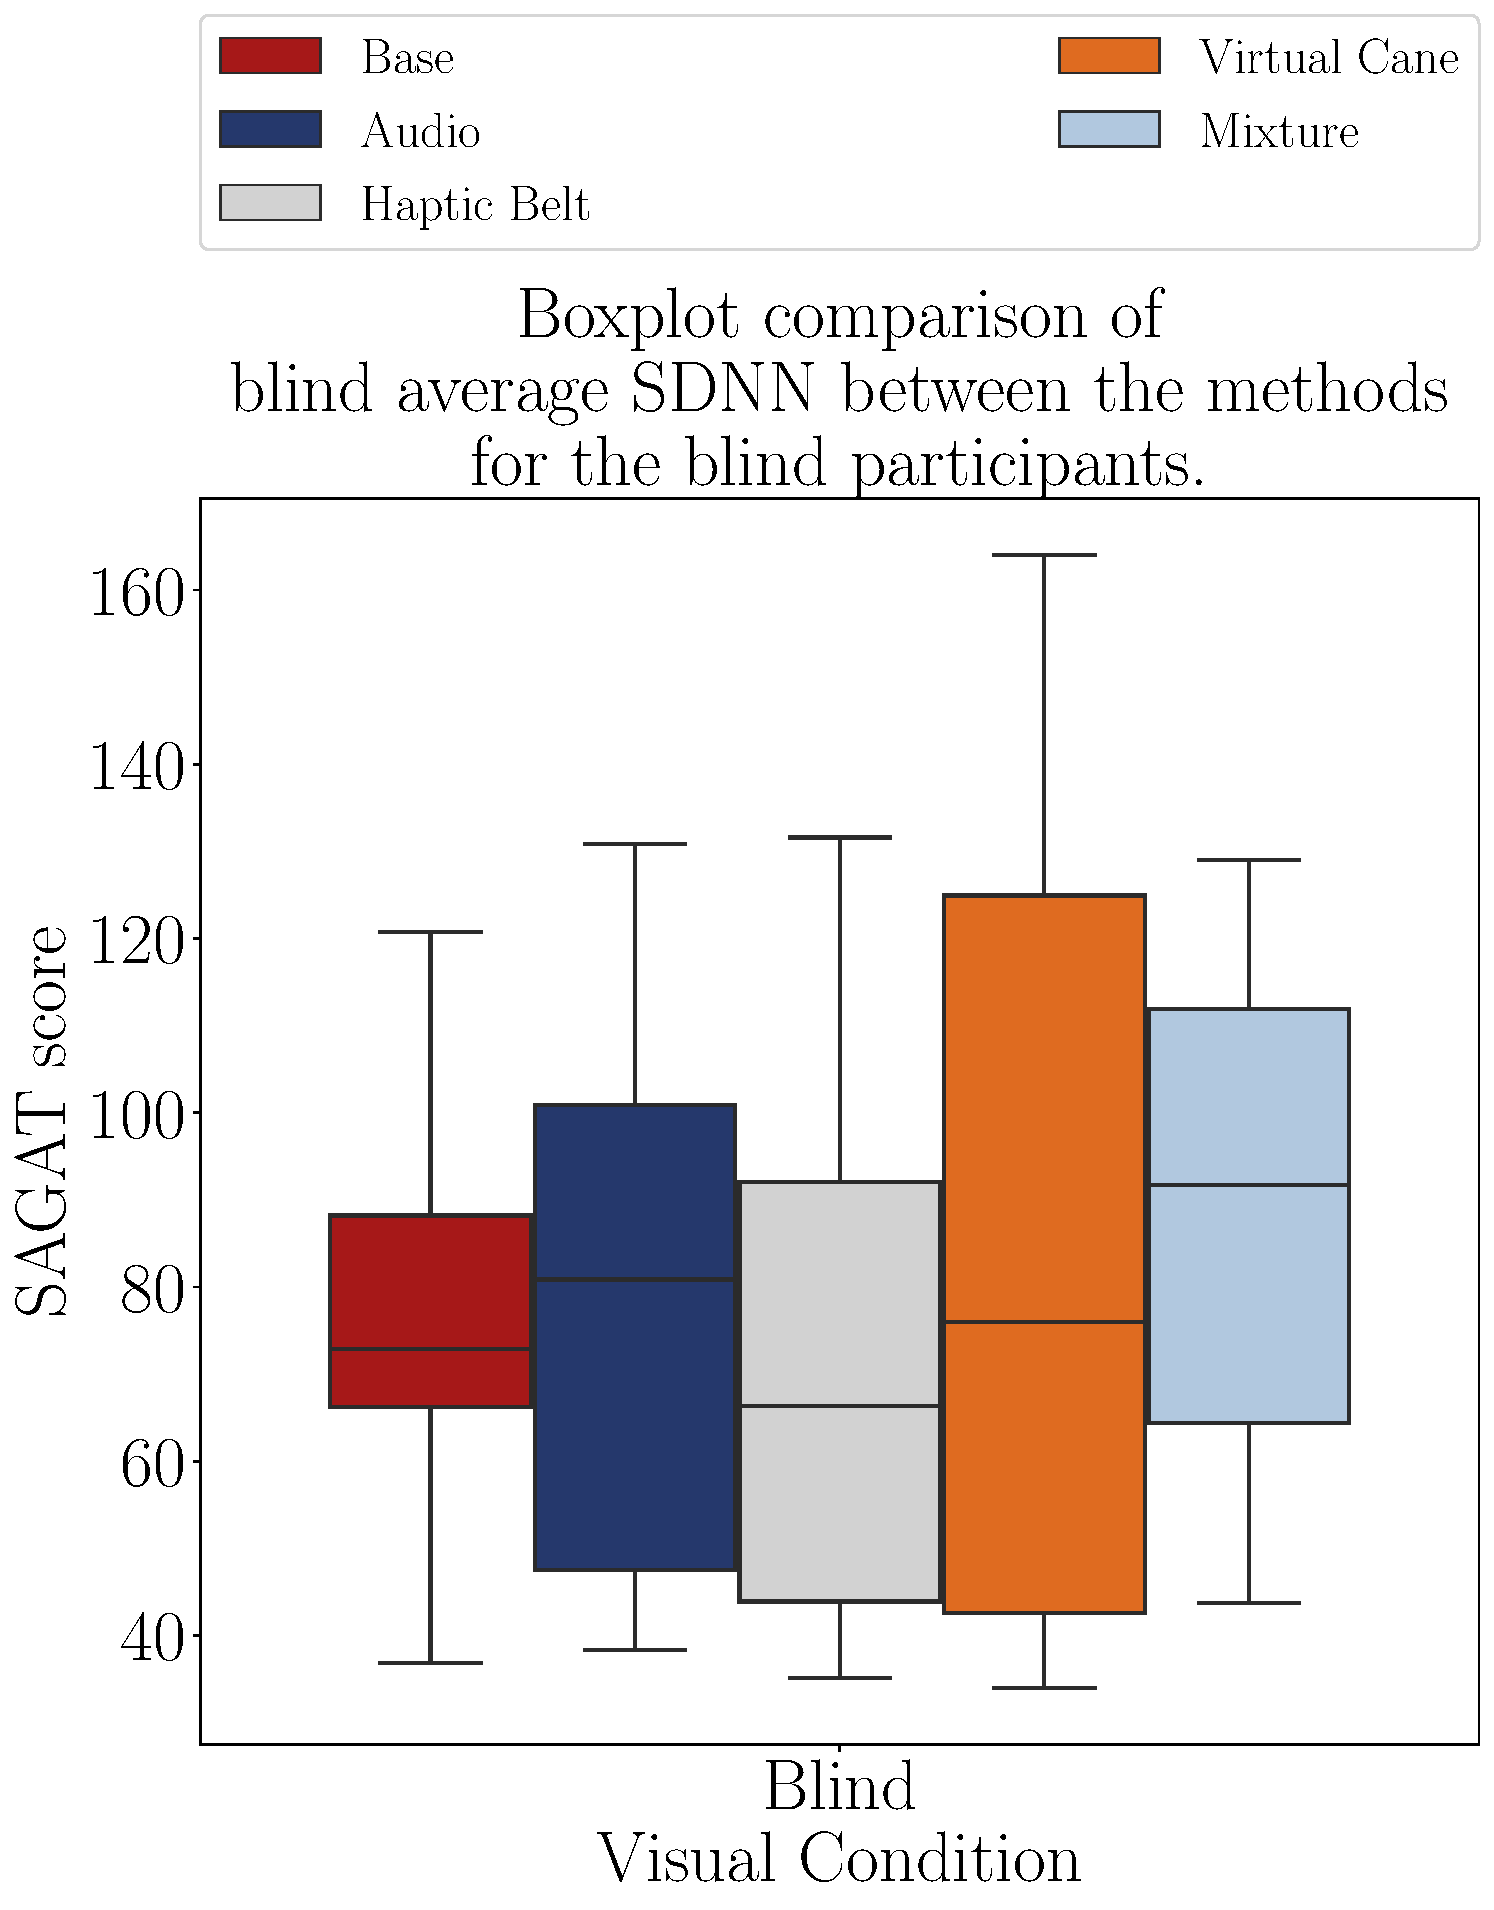
\includegraphics[width = 0.75\linewidth]{3 - Resultados/Figuras/boxplot_ecg_sdnn_blind_scene.pdf}
    \caption{Boxplot of the SDNN of the blind participants grouped by the methods.}
    \label{fig:boxplot_ecg_sdnn_blind_scene}
\end{figure}
\begin{figure}[!htb]
    \centering
    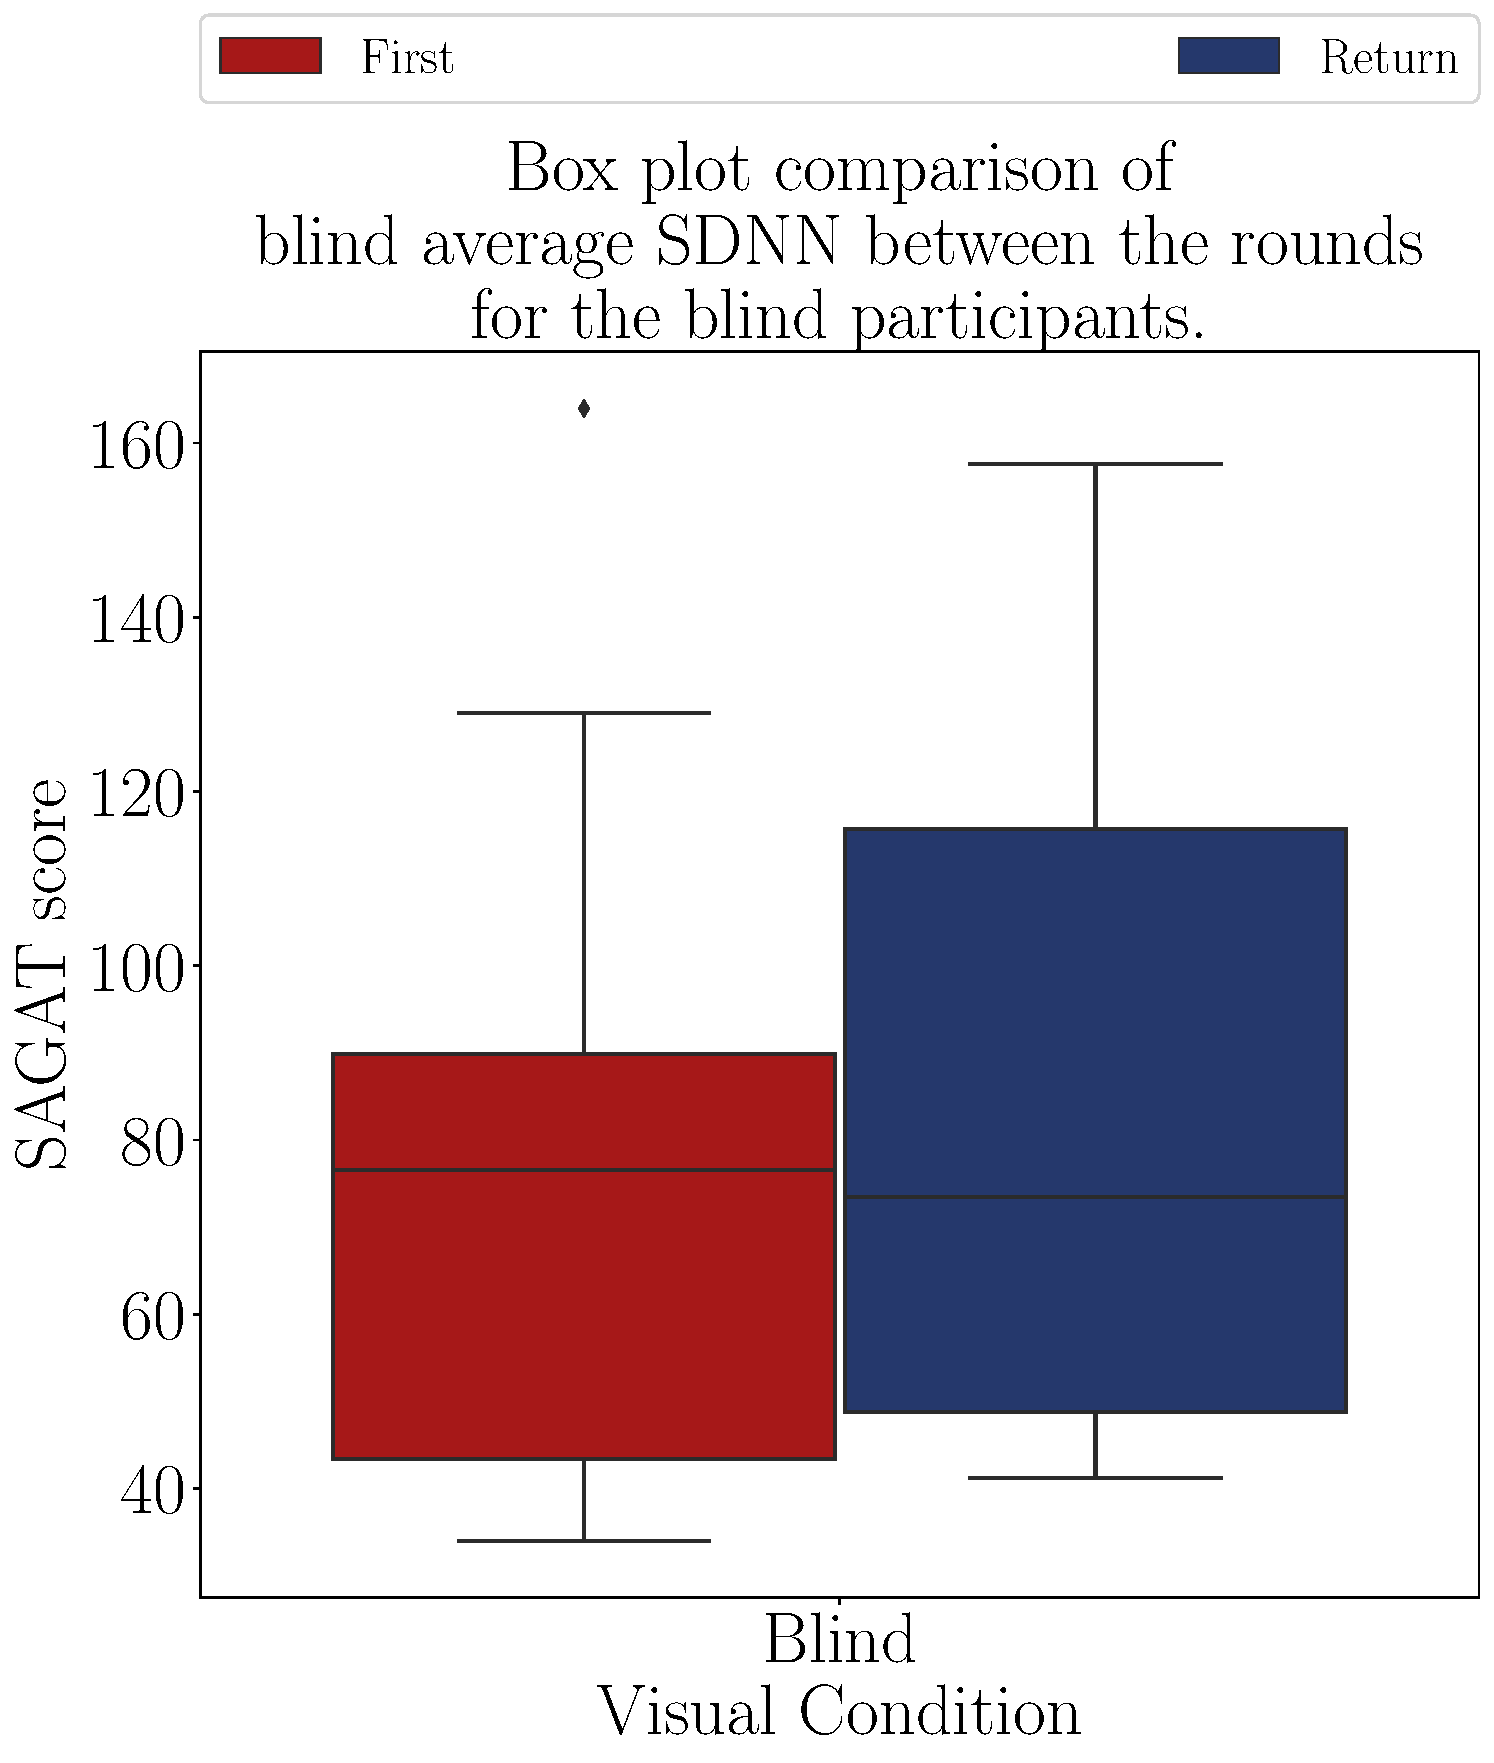
\includegraphics[width = 0.75\linewidth]{3 - Resultados/Figuras/boxplot_ecg_sdnn_blind_rounds.pdf}
    \caption{Boxplot of the SDNN of the blind participants grouped by the rounds.}
    \label{fig:boxplot_ecg_sdnn_blind_rounds}
\end{figure}

The ANOVA results are presented in Table \ref{tab:blocdanova_sdnn_two_way_blind} and do not confirm any influence of the methods nor the rounds on the ECG heart rate variance.


\begin{table}[H]
\centering
\caption{Anova p-value for the average SDNN -- blinded users.}
\label{tab:blocdanova_sdnn_two_way_blind}
\begin{tabular}{lrrrrr}
\toprule
          Source & P-Value \\
\midrule
    \    Methods &   0.486 \\
     \    Rounds &   0.223 \\
\    Interaction &   0.473 \\
\bottomrule
\end{tabular}
\end{table}



\subsubsection{Galvanic skin response and temperature data;}
\label{subsubsec:results_gsr_temp_1}

The GSR analysis is based on the signal's average level. Each experiment's round is compared to the participant baseline collected before the experiment. The GSR sensor was worn on the left hand for right-handed participant and on the right hand for left-handed participants. One of the blind participants had the GSR sensor removed during the experiment because it was not appropriately fixed.

Figure \ref{fig:boxplot_gsr_avg_blind_scene} presents the boxplot of the percentual variation in the skin conductance for each method. The base method has the lowest variation among all methods. Also, the introduction of vibration increases the method variance. Figure \ref{fig:boxplot_gsr_avg_blind_rounds} presents the GSR grouped by the rounds. In this case, there is no apparent difference between the rounds.

\begin{figure}[!htb]
    \centering
    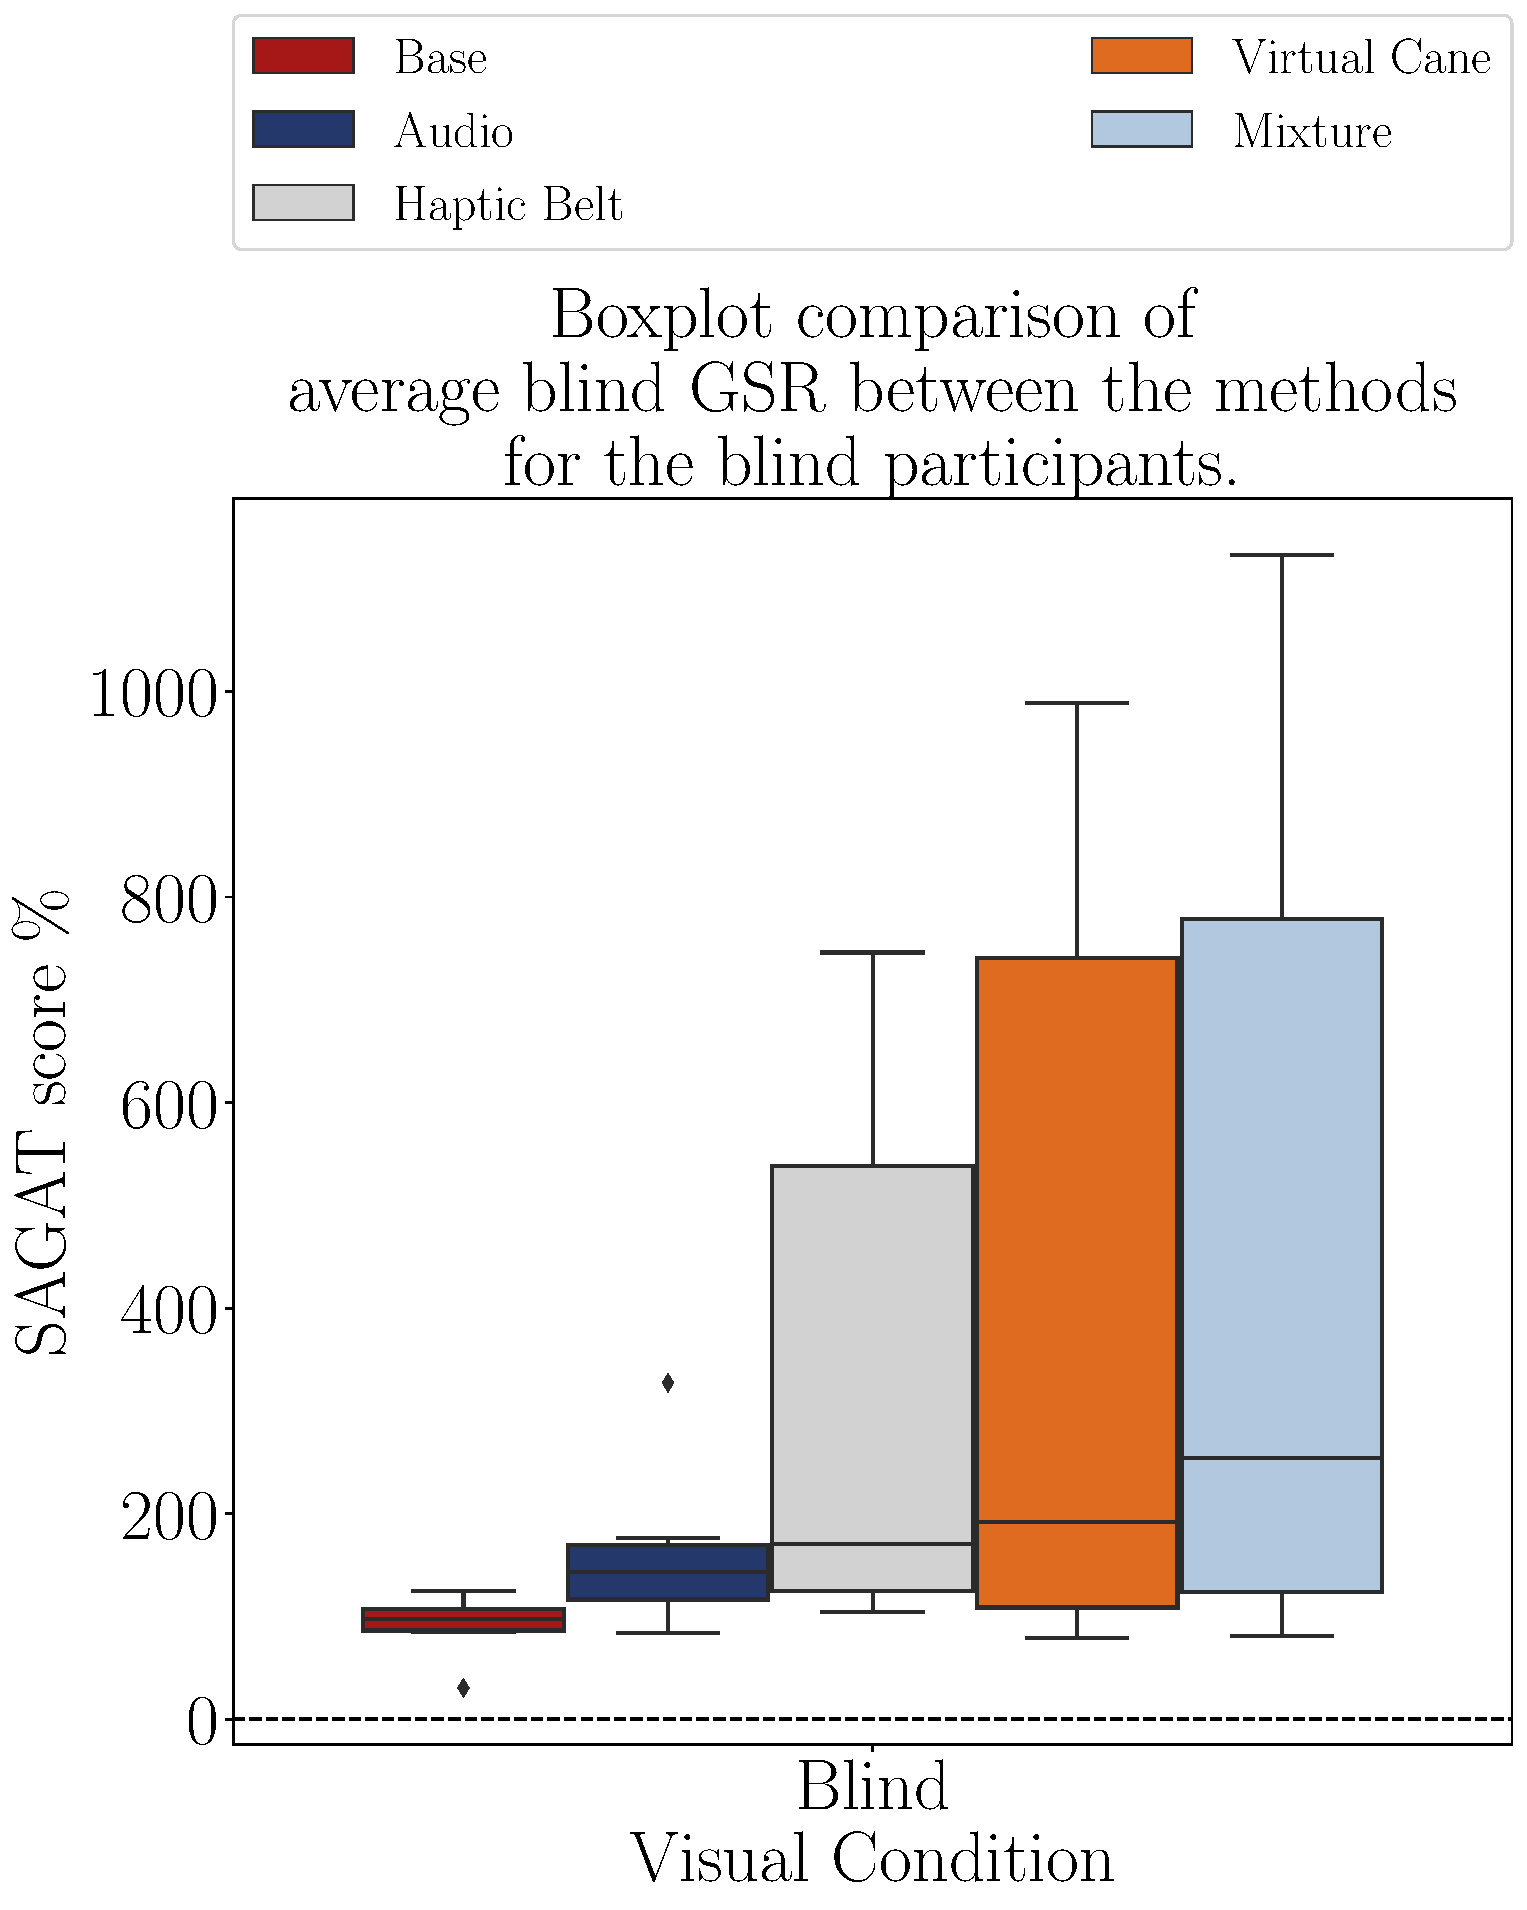
\includegraphics[width = 0.75\linewidth]{3 - Resultados/Figuras/boxplot_gsr_avg_blind_scene.pdf}
    \caption{Boxplot of the GSR of the blind participants grouped by the methods.}
    \label{fig:boxplot_gsr_avg_blind_scene}
\end{figure}
\begin{figure}[!htb]
    \centering
    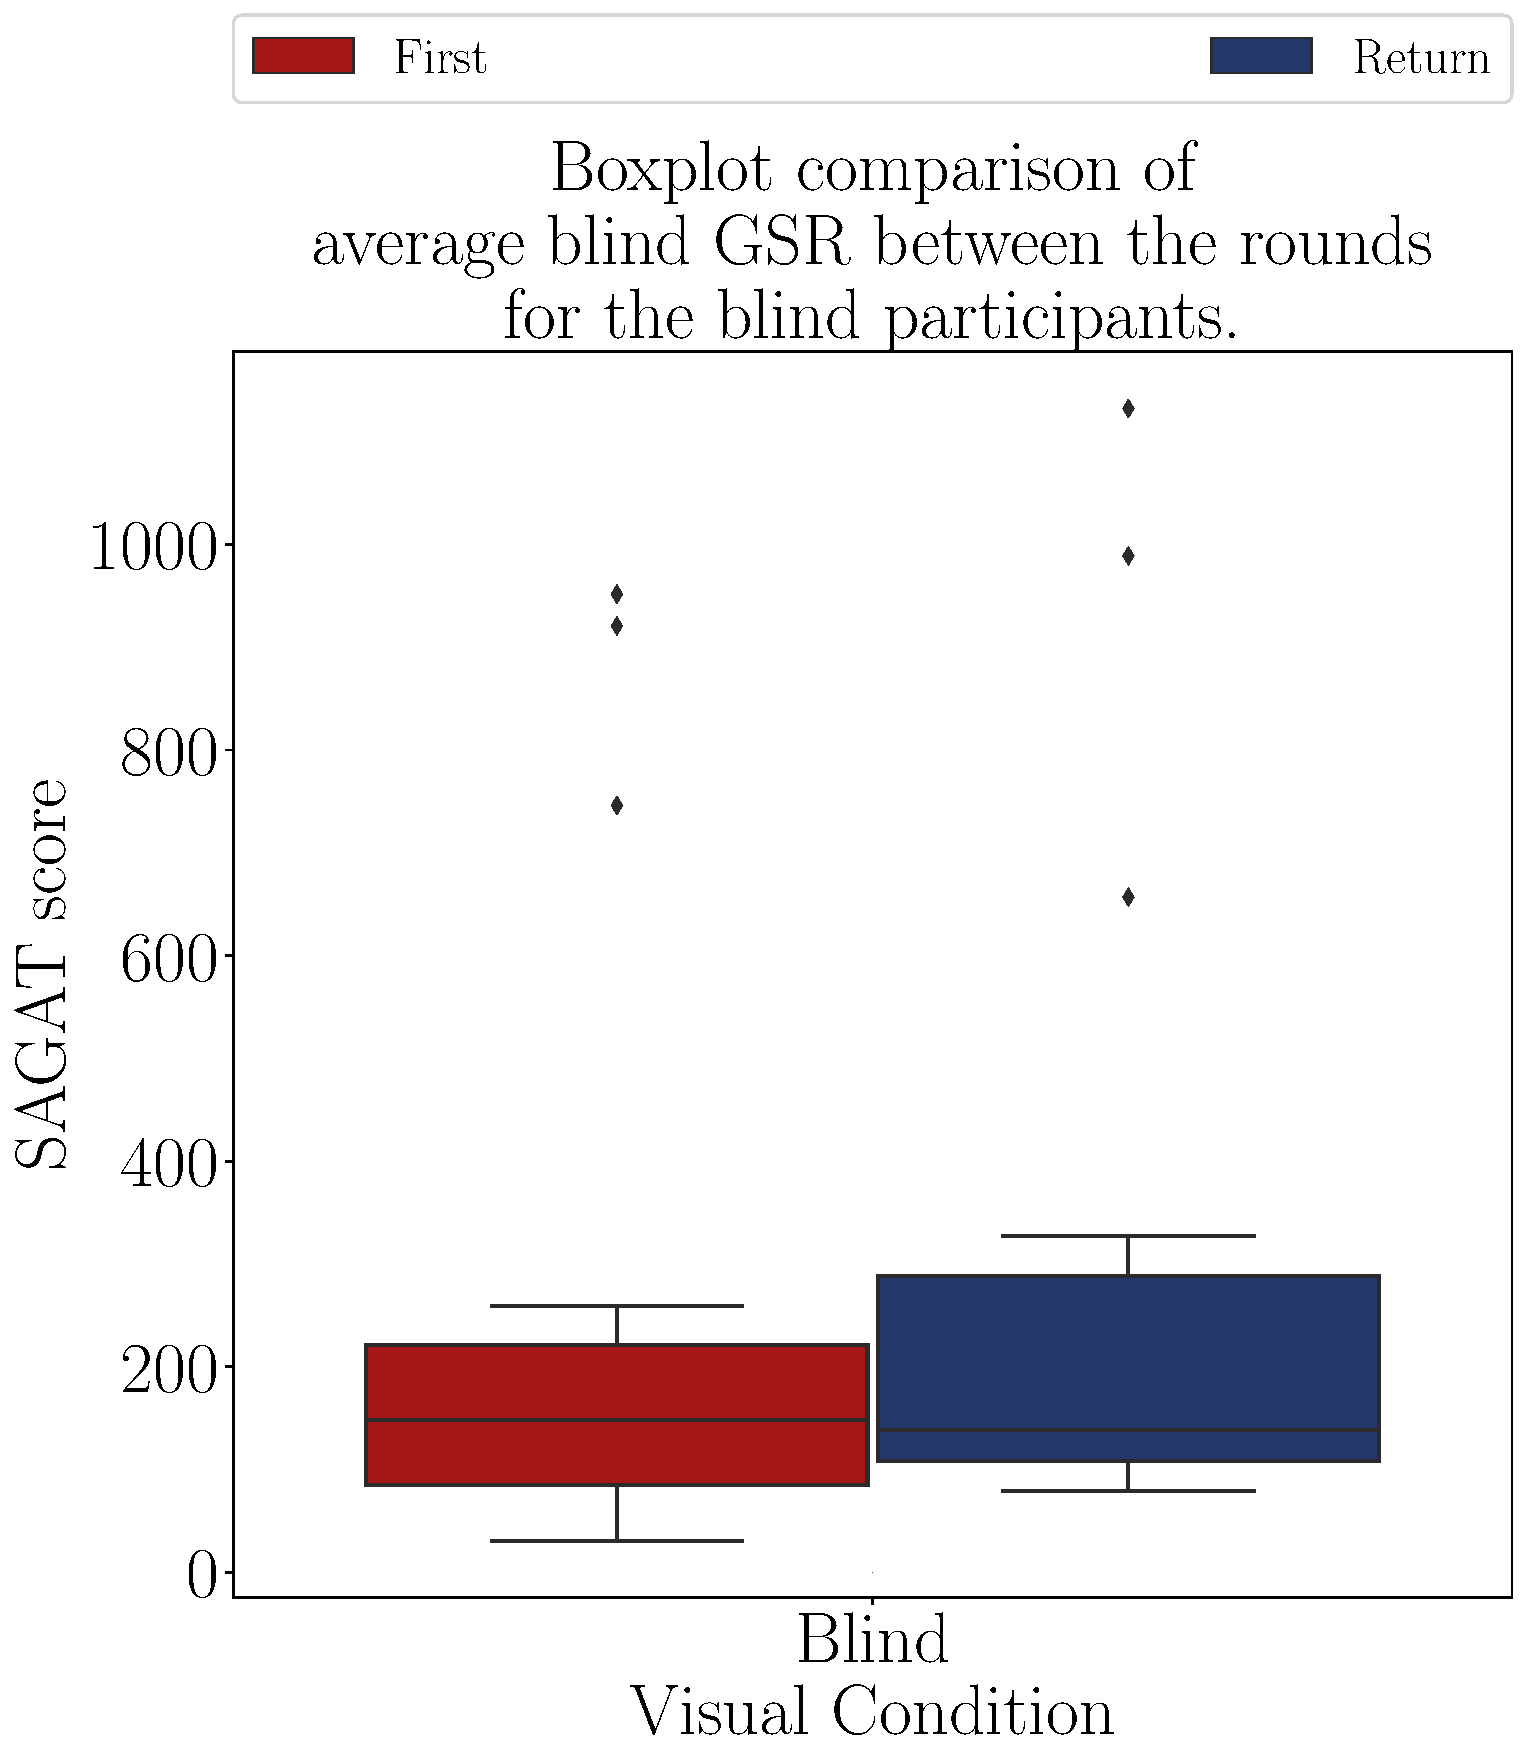
\includegraphics[width = 0.75\linewidth]{3 - Resultados/Figuras/boxplot_gsr_avg_blind_rounds.pdf}
    \caption{Boxplot of the GSR of the blind participants grouped by the rounds.}
    \label{fig:boxplot_gsr_avg_blind_rounds}
\end{figure}

Table \ref{tab:blocanova_gsr_two_way_blind} shows the ANOVA test p-value for the GSR percentual variance. Although the p-value for the method is not below the threshold of 0.05, it is close to it, indicating that probably the GSR is affected by it. 


\begin{table}[!htb]
\centering
\caption{Anova p-value for the mental demand average on each method for blinded users.}
\label{tab:blocanova_gsr_two_way_blind}
\begin{tabular}{lrrrrl}
\toprule
          Source & P-Value \\
\midrule
    \    Methods &   0.051 \\
     \    Rounds &   0.722 \\
\    Interaction &   0.996 \\
\bottomrule
\end{tabular}
\end{table}






%\subsubsection*{Final Remarks}
%
%To summarize the conclusion obtained from the analysis of the data from blind participants, %the audio method showed a lower score both for NASA-TLX mental demand and NASA-TLX global %score. In contrast, the methods that include vibration achieved higher scores. This probably %happened because the participants are already used to using sound to guide themselves, %especially environmental sounds. The environment sounds used in the scenes were always the %same (telephone ringing, laptop keyboard sounds, exterior noise, door opening and closing). %The participants likely felt more relaxed when they only had to focus on the sounds around %him/her. This is reinforced by the fact that, during the experiment with the audio method, %half of the participants did not ask for any information, or the audio command option was %used only a few times.
%
%The fact that the haptic devices caused a higher workload is probably due to the fact that %the users had to learn and get used to them. Besides, for being just conceptual, their %precision was not as good as they were expecting. That explains why their results were not %as good as the base or audio methods. The NASA-TLX results are correctly related to the %satisfaction questionnaires, which scored them as the unsatisfied devices.
%
%As expected, most of the variables from subjective questionnaires (NASA-TLX and SAGAT) show %some influence of the rounds. On the other hand, the results from the physiological sensors %did not show a clear tendency. 
%
%The statistical analysis based on ANOVA tests confirmed some of the observations from the %bar and box plots. However, in many cases, the residual distributions were not homogenous %and the statistical analysis was affected by the small number of samples. 
%
%All the blind participants showed great enthusiasm before, during and after the experiment. %They also made several recommendations for both the virtual environment and the devices, %such as:
%
%\begin{itemize}
%    \item The speakers of the HMD are not good enough to give them the precise location of %the sound origin
%    \item The HMD is too large and covers half of the participant's face. It gives them a strange sensation, since some of them use the air or the wind feeling on the face to give them hints about the location of walls or other high obstacles;
%    \item The precision of the vibration for both the haptic belt and the virtual cane needs to be improved. It is not enough for them to use the devices. This problem is related to %how the HMD sets the position of the user in the virtual environment. \\    
%    \item The vibration from the haptic belt was not intense enough.
%\end%{itemize}

\subsection{Comparison between BVI users and sighted users}
\label{sec:results_obj_2}

This section investigates the second research question of this work: “do non-BVI users, when deprived of their vision, similarly evaluate assistive devices as BVI users?”. 

To do so, the analysis performed in the previous section is now repeated with the data obtained from sighted participants. However, the data corresponding to the "base" method is omitted, as the daily method used by sighted people is based on their vision.

%\subsection{Subjective data}

Only two of the questionnaires will be analyzed, the NASA-TLX and the Adapted SAGAT, and it is expected that for:

\begin{itemize}
    \item \nameref{subsubsec:results_nasa_tlx_2};
    
        There will be a noticeable difference between the sight sample mental workload and the blind sample mental workload.

    \item \nameref{subsubsec:results_adapted_sagat_2};
    
        Is expected to notice a difference between the “blind” sample and the “sight” sample.

    \item \nameref{subsubsec:results_questionnaires}.

        Meant to assess the user experience with each method.

\end{itemize}

\subsection{NASA-TLX}
\label{subsubsec:results_nasa_tlx_2}

\subsubsection{Analysis of the mental demand scale}\mbox{}\\

Table \ref{tab:md_table_noBase} presents the mental demand score of all participants, while the corresponding barplot is presented in Figure \ref{fig:barplot_md_avg_4_scene_blind_sight}. As said before, the higher the value, the higher is the mental demand of the user. It is interesting to observe that sighted people gave a higher score to audio, as they are not so familiar with using sounds as source of guidance.


\begin{table}[!htb]
\centering
\caption{Mental demand felled by the participants.}
\label{tab:md_table_noBase}
\begin{tabular}{lllrrrrr}
\toprule
    &       &        & Audio & \begin{tabular}[c]{@{}l@{}}Haptic\\ Belt\end{tabular} & \begin{tabular}[c]{@{}l@{}}Virtual\\ Cane\end{tabular} & Mixture \\
Participant & \begin{tabular}[c]{@{}l@{}}Visual\\ Condition\end{tabular} & Round &       &                                                       &                                                        &         \\
\midrule
001C & Blind & First &     1 &                                                    14 &                                                      3 &       6 \\
    &       & Return &     1 &                                                    10 &                                                      2 &       6 \\
002C & Blind & First &     1 &                                                     1 &                                                     10 &      12 \\
    &       & Return &     1 &                                                     1 &                                                     10 &       3 \\
003C & Blind & First &     5 &                                                     5 &                                                      8 &       1 \\
    &       & Return &     1 &                                                     1 &                                                      2 &       1 \\
004C & Blind & First &    10 &                                                    15 &                                                     10 &      10 \\
    &       & Return &    10 &                                                    14 &                                                      8 &      10 \\
001 & Sight & First &    12 &                                                    11 &                                                      5 &       9 \\
    &       & Return &    13 &                                                    13 &                                                      5 &      10 \\
003 & Sight & First &    18 &                                                    18 &                                                     16 &      10 \\
    &       & Return &    12 &                                                    15 &                                                     11 &       8 \\
004 & Sight & First &    17 &                                                    20 &                                                     12 &      20 \\
    &       & Return &    12 &                                                    15 &                                                     10 &      15 \\
005 & Sight & First &     4 &                                                    12 &                                                     10 &      13 \\
    &       & Return &     6 &                                                    10 &                                                      6 &      12 \\
\bottomrule
\end{tabular}
\end{table}



\begin{figure}[!thb]
    \centering
    \begin{minipage}{\textwidth}
        \centering
        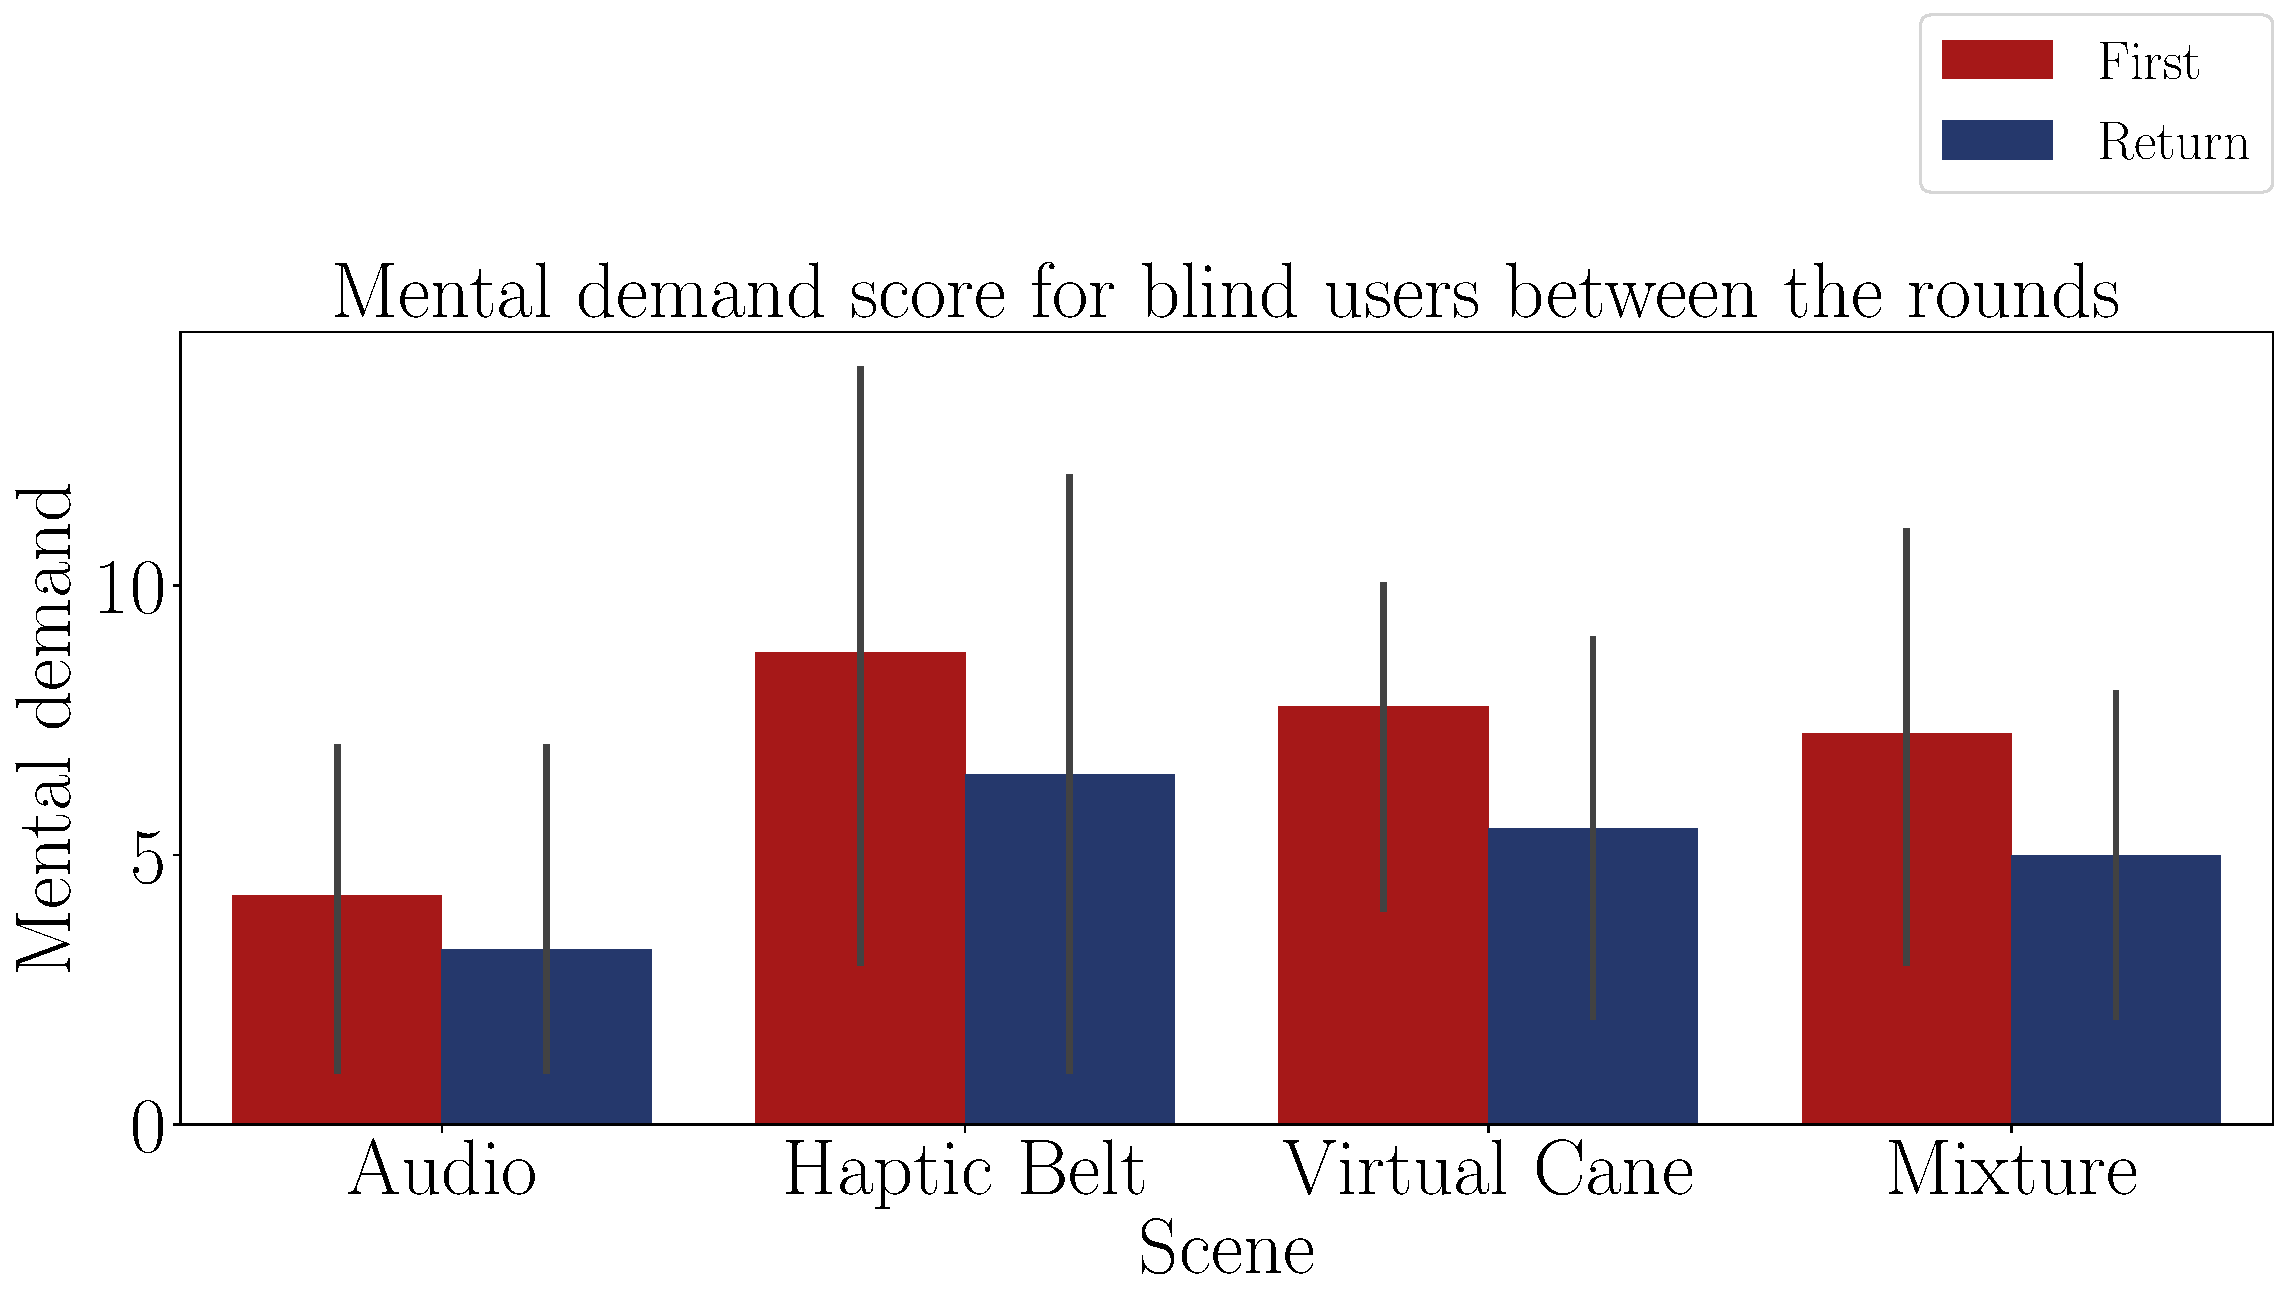
\includegraphics[width = \textwidth]{Resultados/Nasa/Figuras/pdf/barplot_md_avg_4_scene_blind.pdf}
        \subcaption{Blind participants}
        \label{fig:barplot_md_avg_4_scene_blind}
    \end{minipage}
    \begin{minipage}{\textwidth}
        \centering
        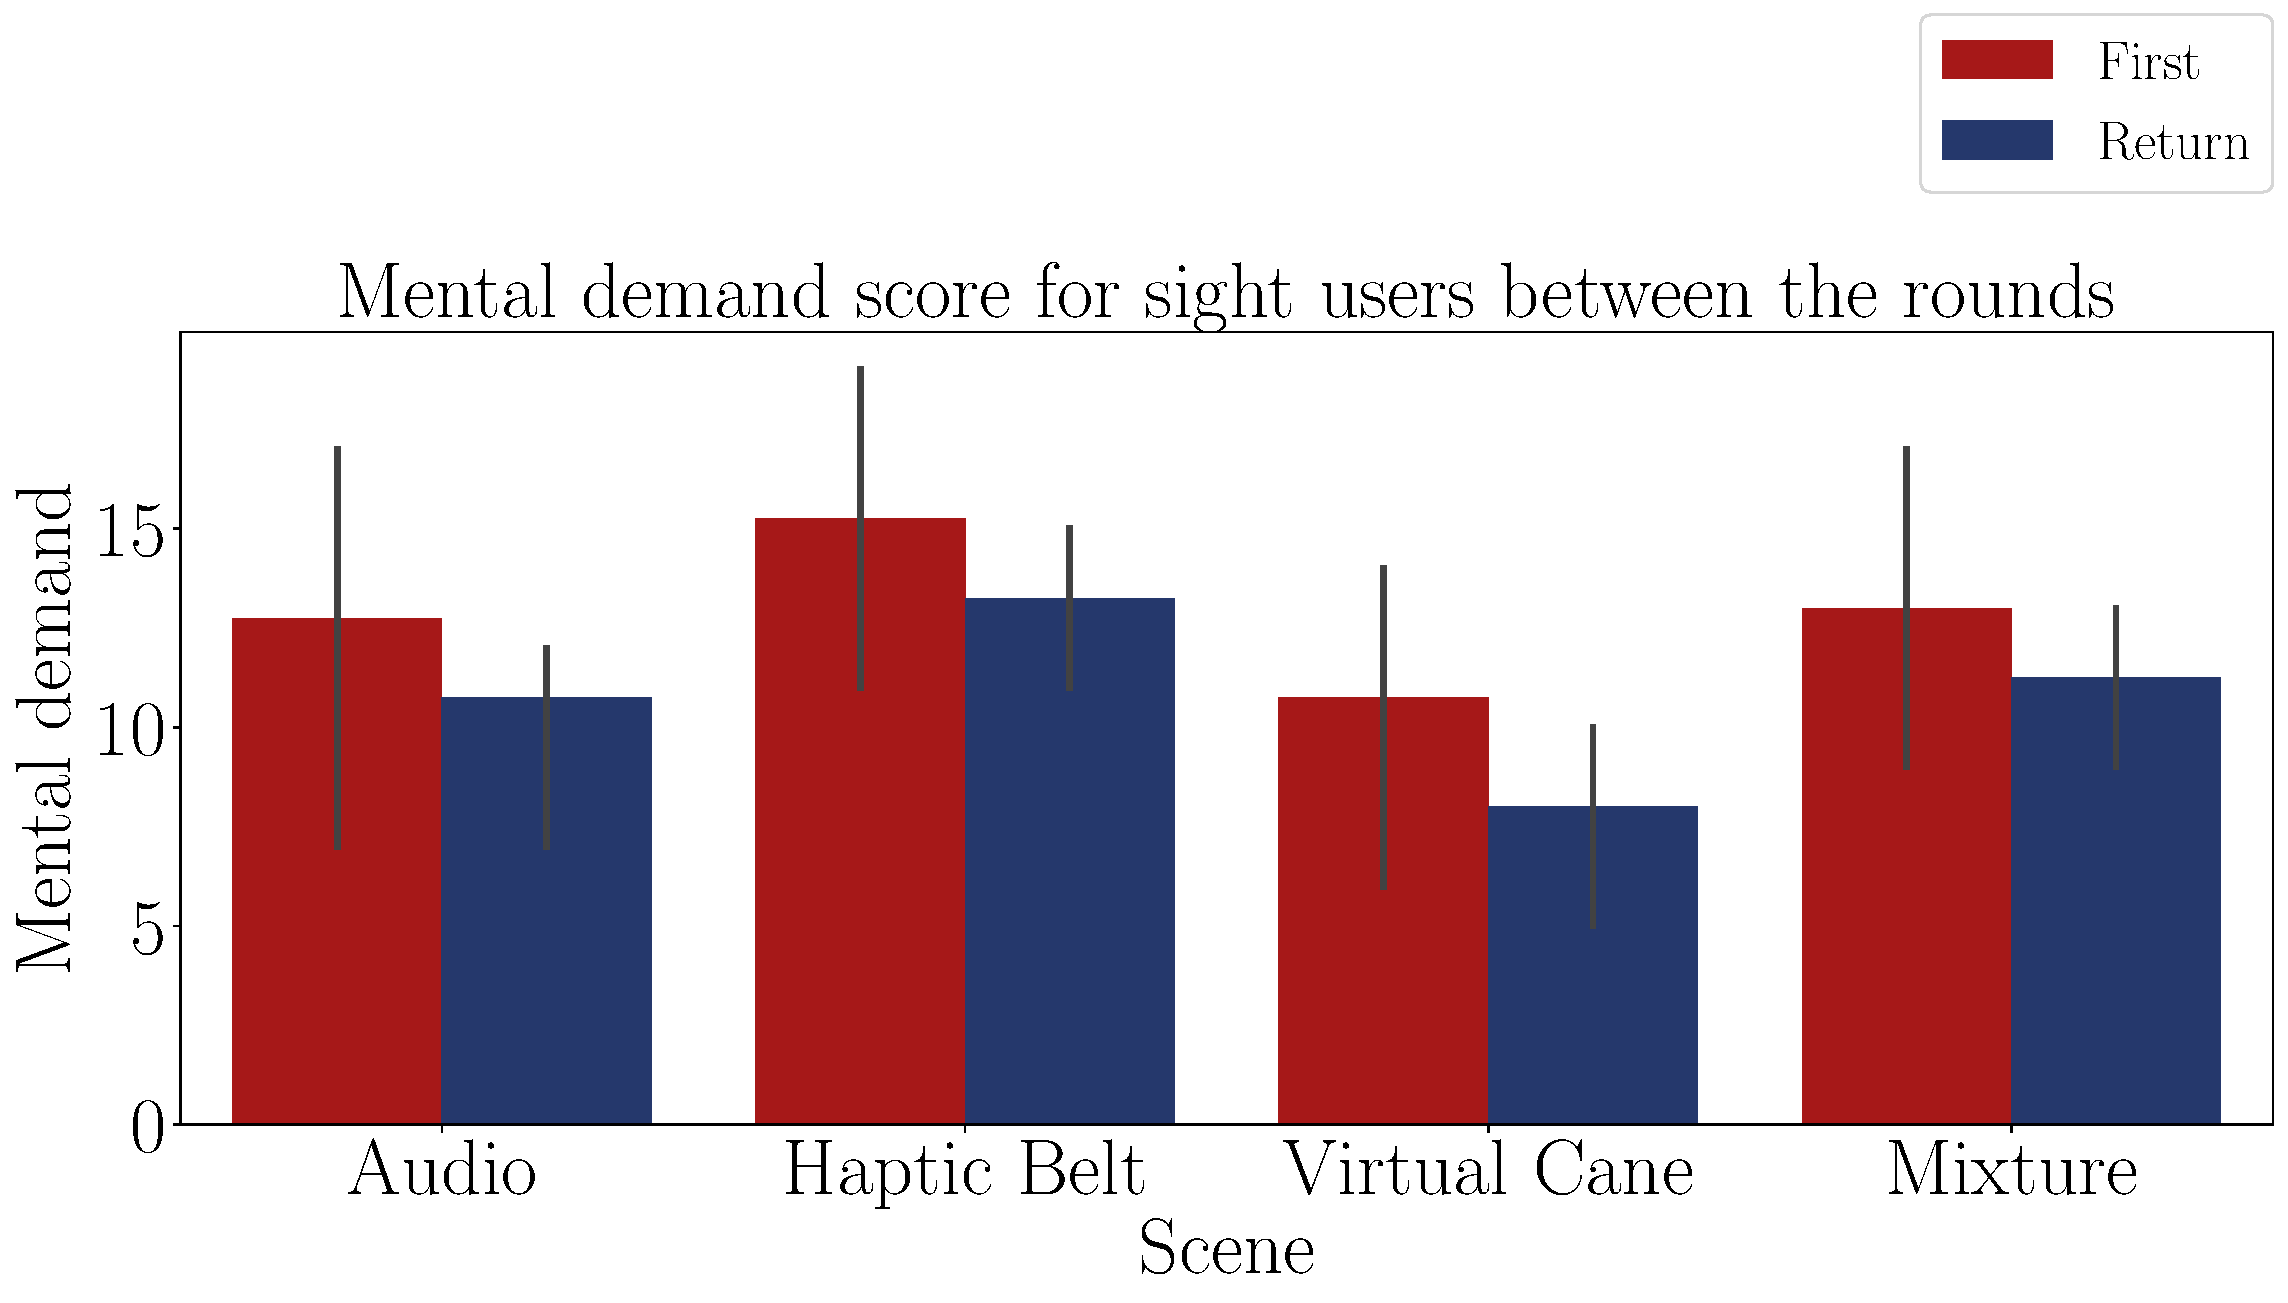
\includegraphics[width = \textwidth]{Resultados/Nasa/Figuras/pdf/barplot_md_avg_4_scene_sight.pdf}
        \subcaption{Sight participants}
        \label{fig:barplot_md_avg_4_scene_sight}
    \end{minipage}
    \caption{Barplot of the average mental demand on each method and each round.}
    \label{fig:barplot_md_avg_4_scene_blind_sight}
\end{figure}

Figures \ref{fig:boxplot_noBase_md_4_scene} and \ref{fig:boxplot_noBase_md_4_rounds} presents the box plot for both groups, organized by the methods and the rounds. The mental demand is systematically higher for sighted people, which is expected. However, while blind participants considered the audio method less demanding, sighted participants prefered to the virtual cane. For both groups, we observe a decrease in the mental demand.

\begin{figure}[!htb]
    \centering
    \begin{minipage}{0.45\textwidth}
        \centering
        \includegraphics[width = \textwidth]{Resultados/Nasa/Figuras/pdf/boxplot_noBase_md_4_scene.pdf}
        \caption{Boxplot of the mental demand of the participants grouped by the methods.}
        \label{fig:boxplot_noBase_md_4_scene}
    \end{minipage}
    \begin{minipage}{0.075\textwidth}
        \hfill
    \end{minipage}
    \begin{minipage}{0.45\textwidth}
        \centering
        \includegraphics[width = \textwidth]{Resultados/Nasa/Figuras/pdf/boxplot_noBase_md_4_rounds.pdf}
        \caption{Boxplot of the mental demand of the participants grouped by the rounds.}
        \label{fig:boxplot_noBase_md_4_rounds}
    \end{minipage}
\end{figure}

Figures \ref{fig:qqplot_md_avg_two_way_sight} and \ref{fig:residplot_md_avg_two_way_sight} show the QQ plot and residual distribution for the sighted data, confirming that the data is normally distributed and participants have similar variance. Table \ref{tab:blocanova_md_avg_two_way_blind_sight} brings the results of ANOVA. Unlike the blind participants, in the case of sighted ones, the p-value for the methods is below the threshold of 0.05, confirming it as a significant variable for the mental demand. In the case of the rounds, the data from both sighted and blind participants resulted in the exact p-value of 0.075, which is close to the traditional threshold of 0.05 but slightly higher. 

\begin{table}[!htb]
    \caption{Anova p-value for the mental demand average on each method'}
    \label{tab:blocanova_md_avg_two_way_blind_sight}
\begin{minipage}{0.45\textwidth}
    \subcaption{Blind participants}
    
\centering
\begin{tabular}{ll}
\toprule
          Source & P-Value \\
\midrule
    \    Methods &   0.170 \\
     \    Rounds &   0.075 \\
\    Interaction &   0.993 \\
\bottomrule
\end{tabular}

\end{minipage}
\begin{minipage}{0.45\textwidth}
    \subcaption{Sight participants}
    
\centering
\begin{tabular}{ll}
\toprule
          Source & P-Value \\
\midrule
    \    Methods & 0.049** \\
     \    Rounds &   0.075 \\
\    Interaction &   0.990 \\
\bottomrule
\end{tabular}
    
\end{minipage}
\end{table}

\begin{figure}[!htb]
    \centering
    %\vspace{-15.0cm}
    \begin{minipage}{0.45\textwidth}
        \centering
        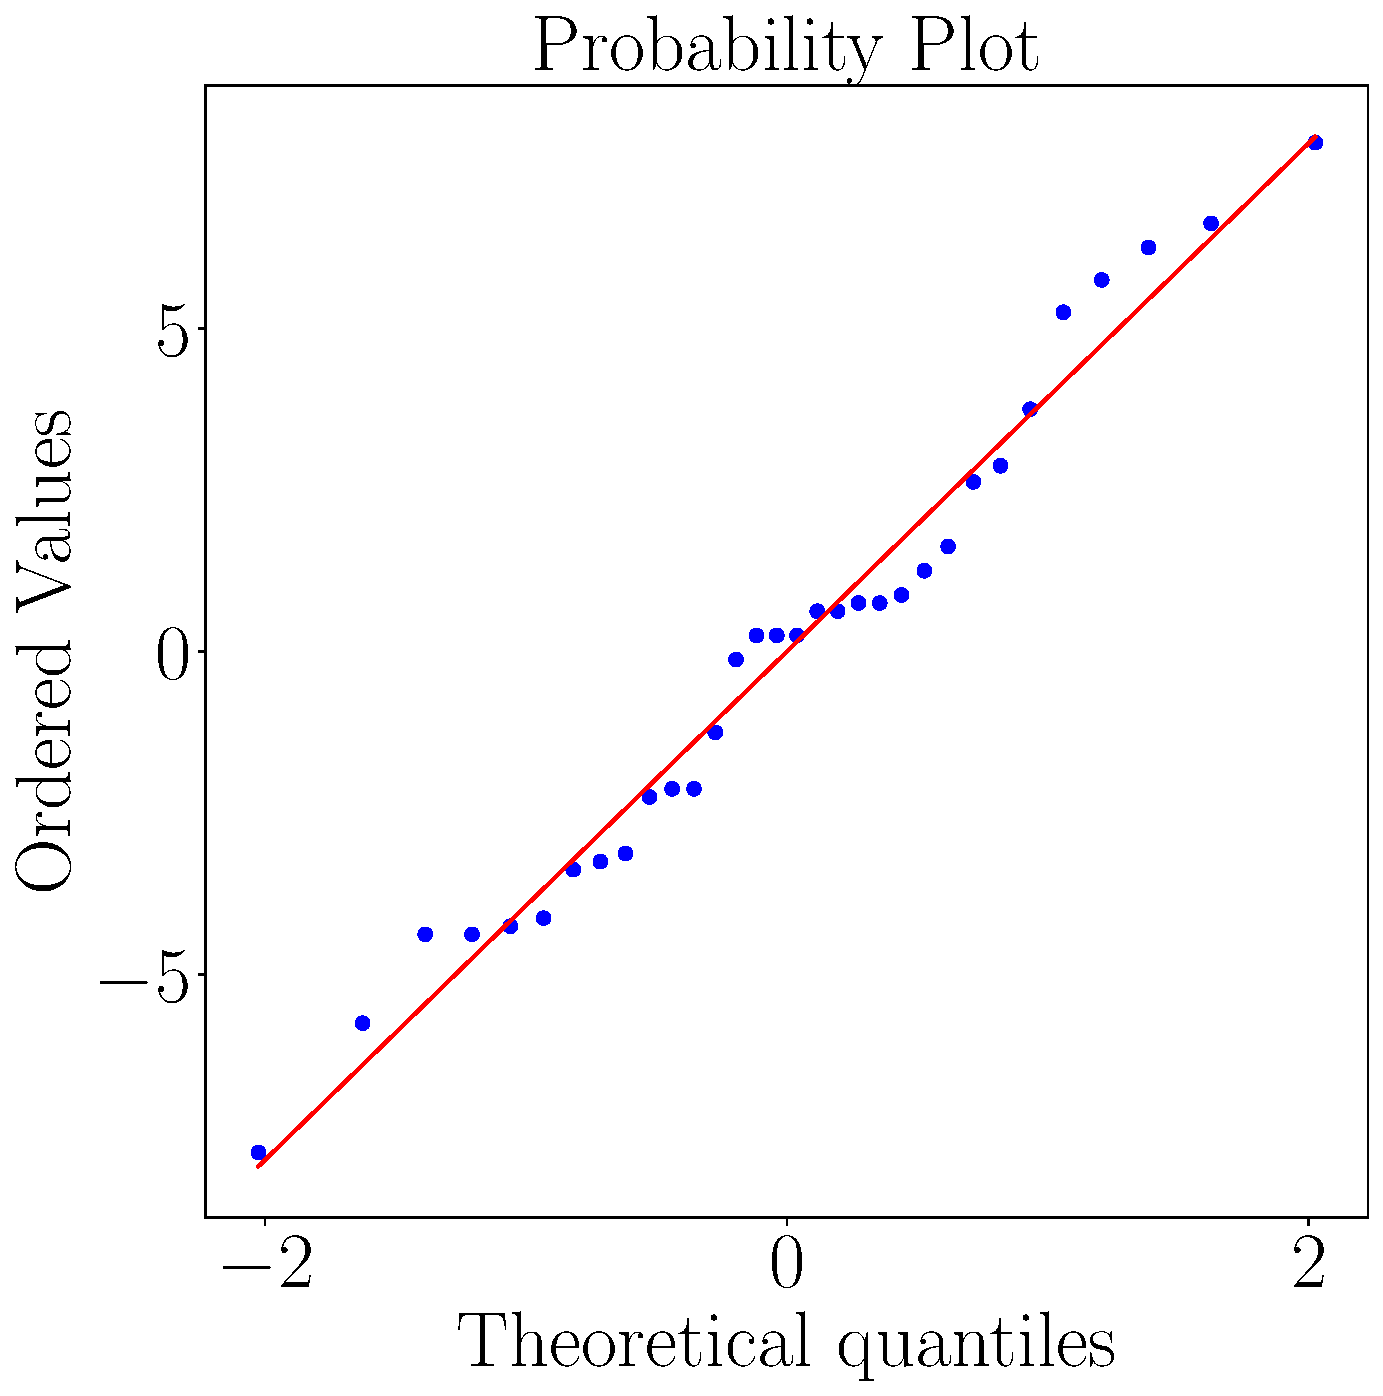
\includegraphics[width = \textwidth]{Resultados/Nasa/Figuras/pdf/qqplot_md_avg_two_way_sight.pdf}
        \caption{QQ plot of the mental demand of the sight participants on each method.}
        \label{fig:qqplot_md_avg_two_way_sight}
    \end{minipage}
    \begin{minipage}{0.075\textwidth}
        \hfill
    \end{minipage}
    \begin{minipage}{0.45\textwidth}
        \centering
        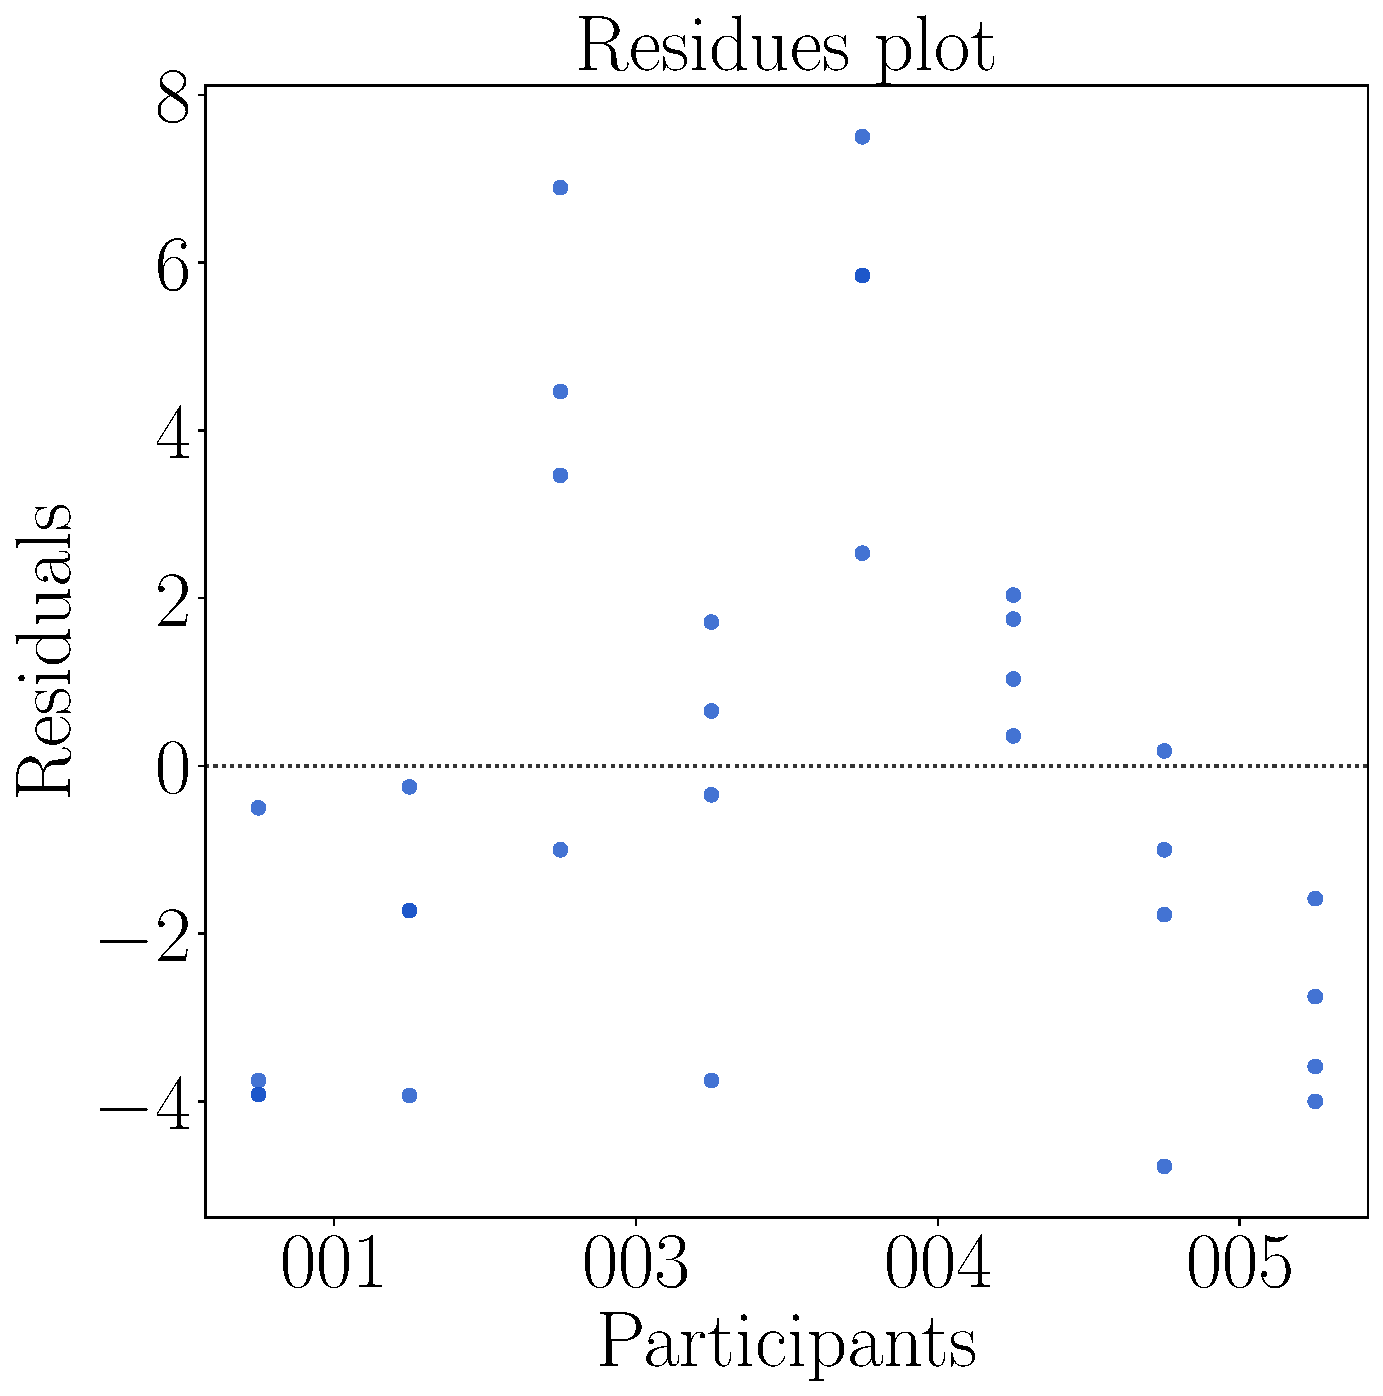
\includegraphics[width = \textwidth]{Resultados/Nasa/Figuras/pdf/residplot_md_avg_two_way_sight.pdf}
        \caption{Residual plot of the mental demand score the sighted participants on each method.}
        \label{fig:residplot_md_avg_two_way_sight}
    \end{minipage}
\end{figure}

\FloatBarrier

%%%%%%%%%%%%%%%%%%%%%%%%%%%%%%%%%%%%%%%%%%%%%%%%%%%%%%%%%%%%%%%%%%%%%%%%%%%%
%%%%%%%%%%%%%%%%%%%%%%%%%%%%%%%%%%%%%%%%%%%%%%%%%%%%%%%%%%%%%%%%%%%%%%%%%%%%
%%%%%%%%%%%%%%%%%%%%%%%%%%%%%%%%%%%%%%%%%%%%%%%%%%%%%%%%%%%%%%%%%%%%%%%%%%%%
%%%%%%%%%%%%%%%%%%%%%%%%%%%%%%%%%%%%%%%%%%%%%%%%%%%%%%%%%%%%%%%%%%%%%%%%%%%%


\subsubsection{Analysis of the NASA-TLX score}\mbox{}\\

Table \ref{tab:nasa_table_noBase} brings the NASA-TLX global score of all participants, while the corresponding barplot is presented in Figure \ref{fig:barplot_nasa_avg_4_scene}. As before, the higher the value, the higher is the Mental Workload of the user.


\begin{table}[!htb]
\centering
\caption{NASA-TLX score felled by the participants.}
\label{tab:nasa_table_noBase}
\begin{tabular}{lllrrrrr}
\toprule
    &       &        &  Audio & \begin{tabular}[c]{@{}l@{}}Haptic\\ Belt\end{tabular} & \begin{tabular}[c]{@{}l@{}}Virtual\\ Cane\end{tabular} & Mixture \\
Participant & \begin{tabular}[c]{@{}l@{}}Visual\\ Condition\end{tabular} & Round &        &                                                       &                                                        &         \\
\midrule
001C & Blind & First &  4.000 &                                                 8.833 &                                                  5.167 &   6.333 \\
    &       & Return &  4.000 &                                                 6.667 &                                                  4.500 &   6.167 \\
002C & Blind & First &  4.833 &                                                 4.833 &                                                  9.000 &   7.000 \\
    &       & Return &  4.833 &                                                 4.833 &                                                  7.000 &   5.167 \\
003C & Blind & First &  4.000 &                                                 5.333 &                                                  6.667 &   3.500 \\
    &       & Return &  3.833 &                                                 3.667 &                                                  3.500 &   3.500 \\
004C & Blind & First & 10.000 &                                                12.667 &                                                  9.667 &  11.000 \\
    &       & Return &  9.167 &                                                11.667 &                                                  9.333 &  10.833 \\
001 & Sight & First & 10.167 &                                                 9.833 &                                                  7.000 &   9.000 \\
    &       & Return & 11.000 &                                                10.833 &                                                  6.167 &   9.333 \\
003 & Sight & First &  9.833 &                                                10.167 &                                                  9.500 &   6.500 \\
    &       & Return &  6.667 &                                                 9.667 &                                                  7.833 &   4.833 \\
004 & Sight & First & 14.833 &                                                13.667 &                                                 11.500 &  15.833 \\
    &       & Return & 11.833 &                                                11.833 &                                                 10.833 &  12.167 \\
005 & Sight & First &  7.667 &                                                 9.000 &                                                  8.000 &   9.667 \\
    &       & Return &  7.667 &                                                 8.667 &                                                  7.667 &   6.000 \\
\bottomrule
\end{tabular}
\end{table}



From Figure \ref{fig:barplot_nasa_avg_4_scene}, it is possible to see that, similar to blind participants, sighted participants consider that the workload of the return round was lower than that of the first round. However, similar to what happened for the mental demand, sighted participants considered virtual cane as the methods with the lowest workload, while, for  blind participants, it was the audio.

\begin{figure}[!htb]
    \centering
    \begin{minipage}{\textwidth}
        \centering
        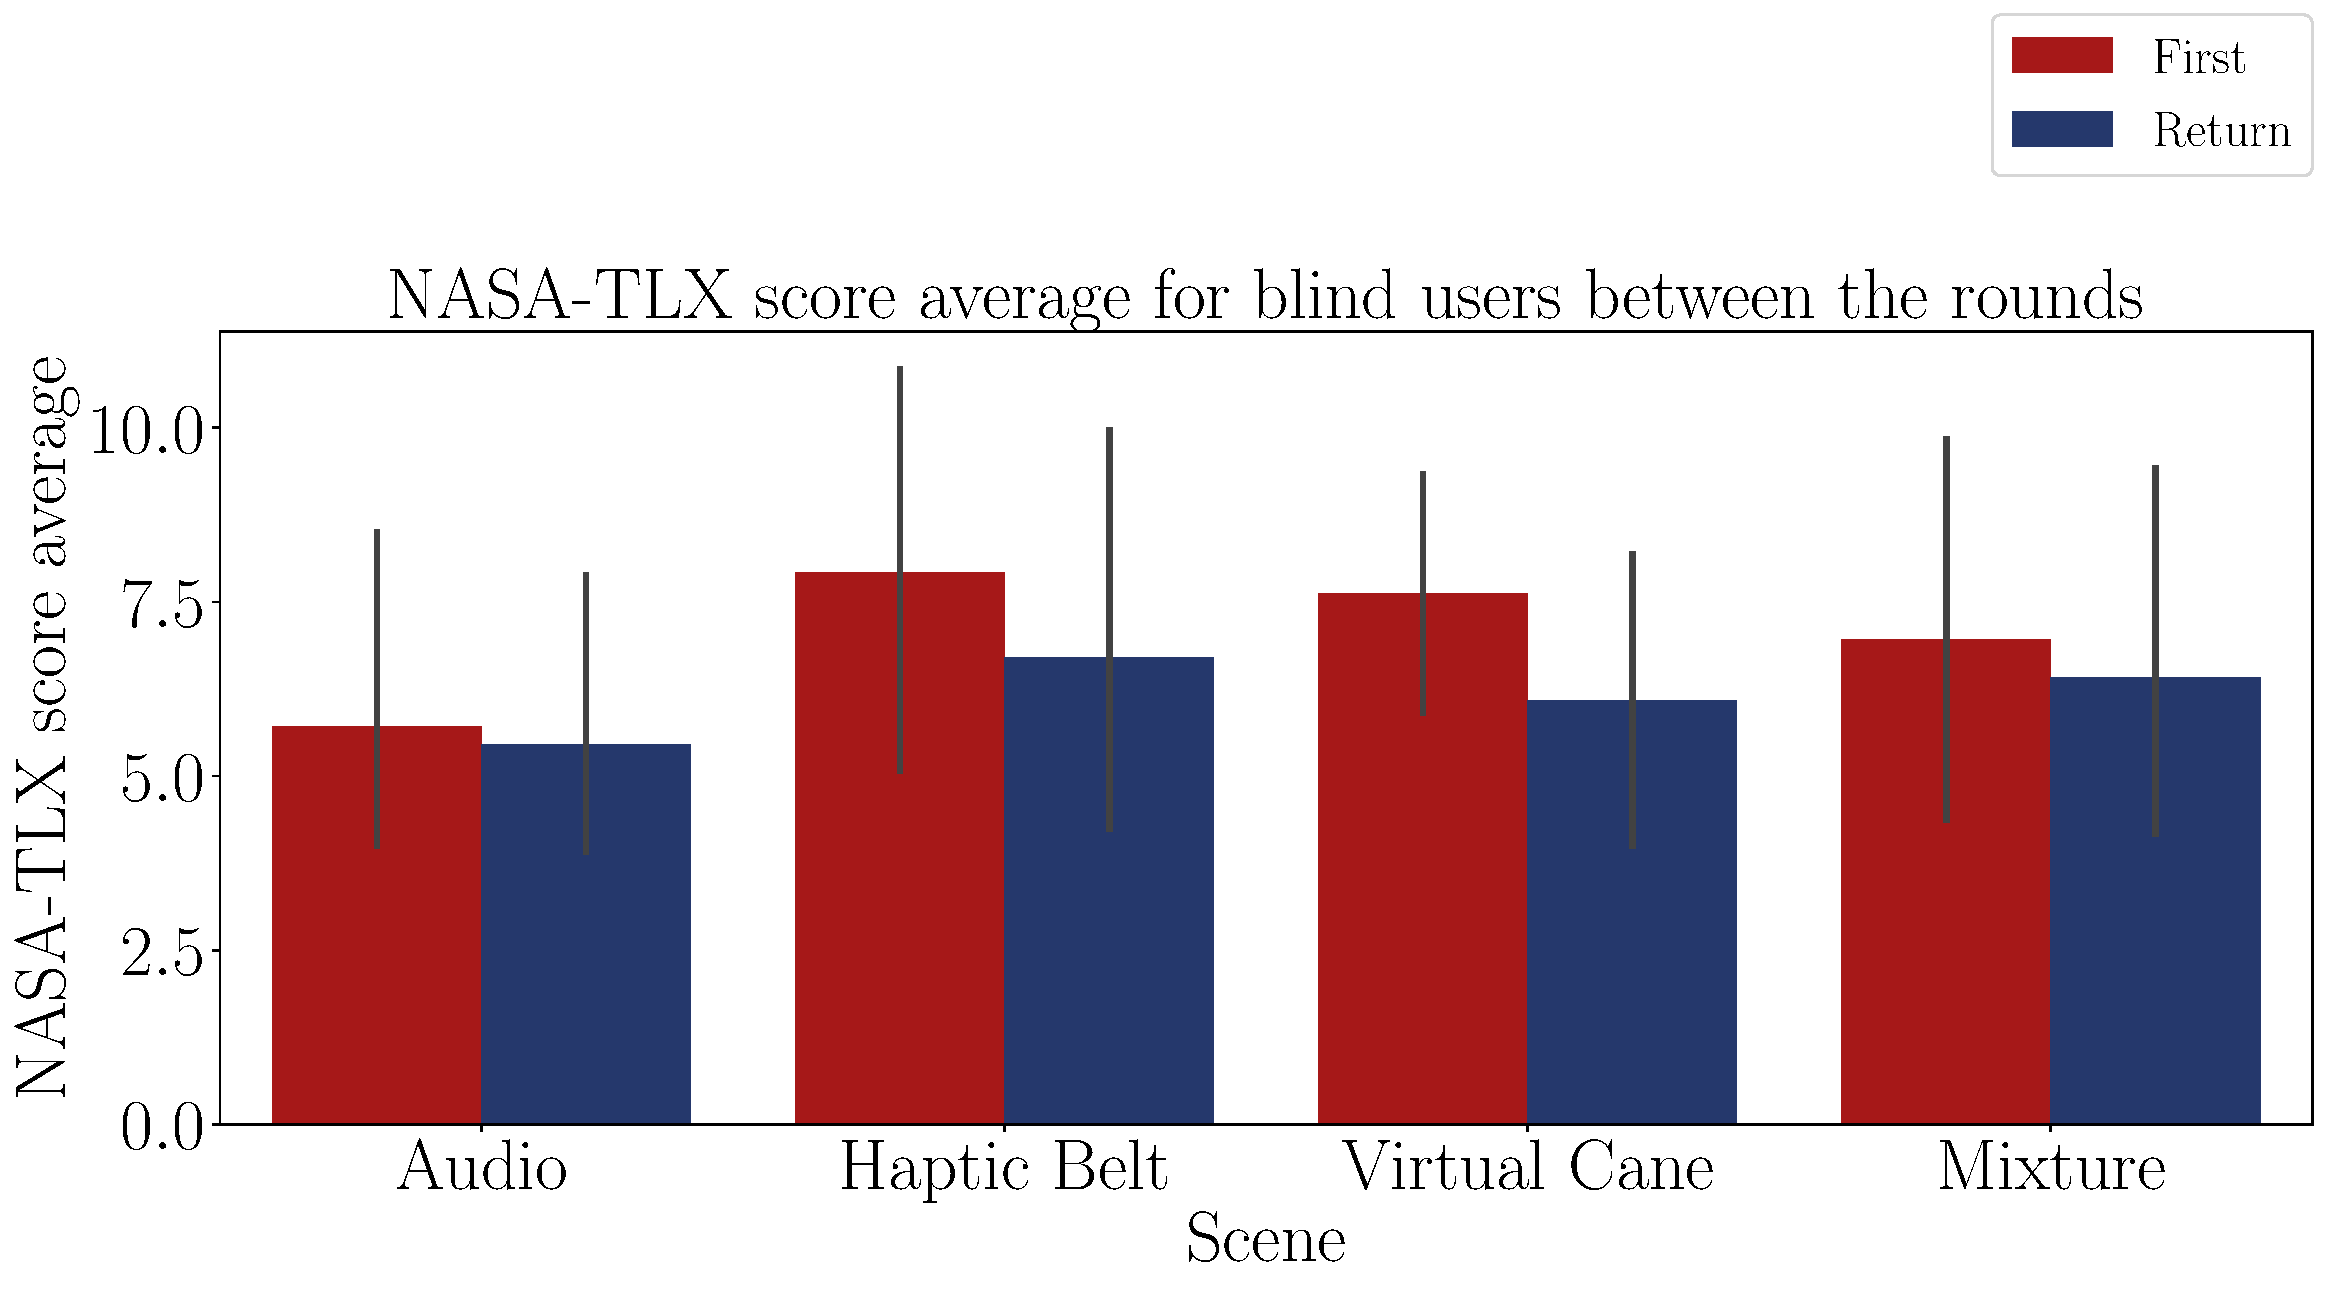
\includegraphics[width = \textwidth]{Resultados/Nasa/Figuras/pdf/barplot_nasa_avg_4_scene_blind.pdf}
        \subcaption{Blind participants.}
        \label{fig:barplot_nasa_avg_4_scene_blind}
    \end{minipage}
    \begin{minipage}{\textwidth}
        \centering
        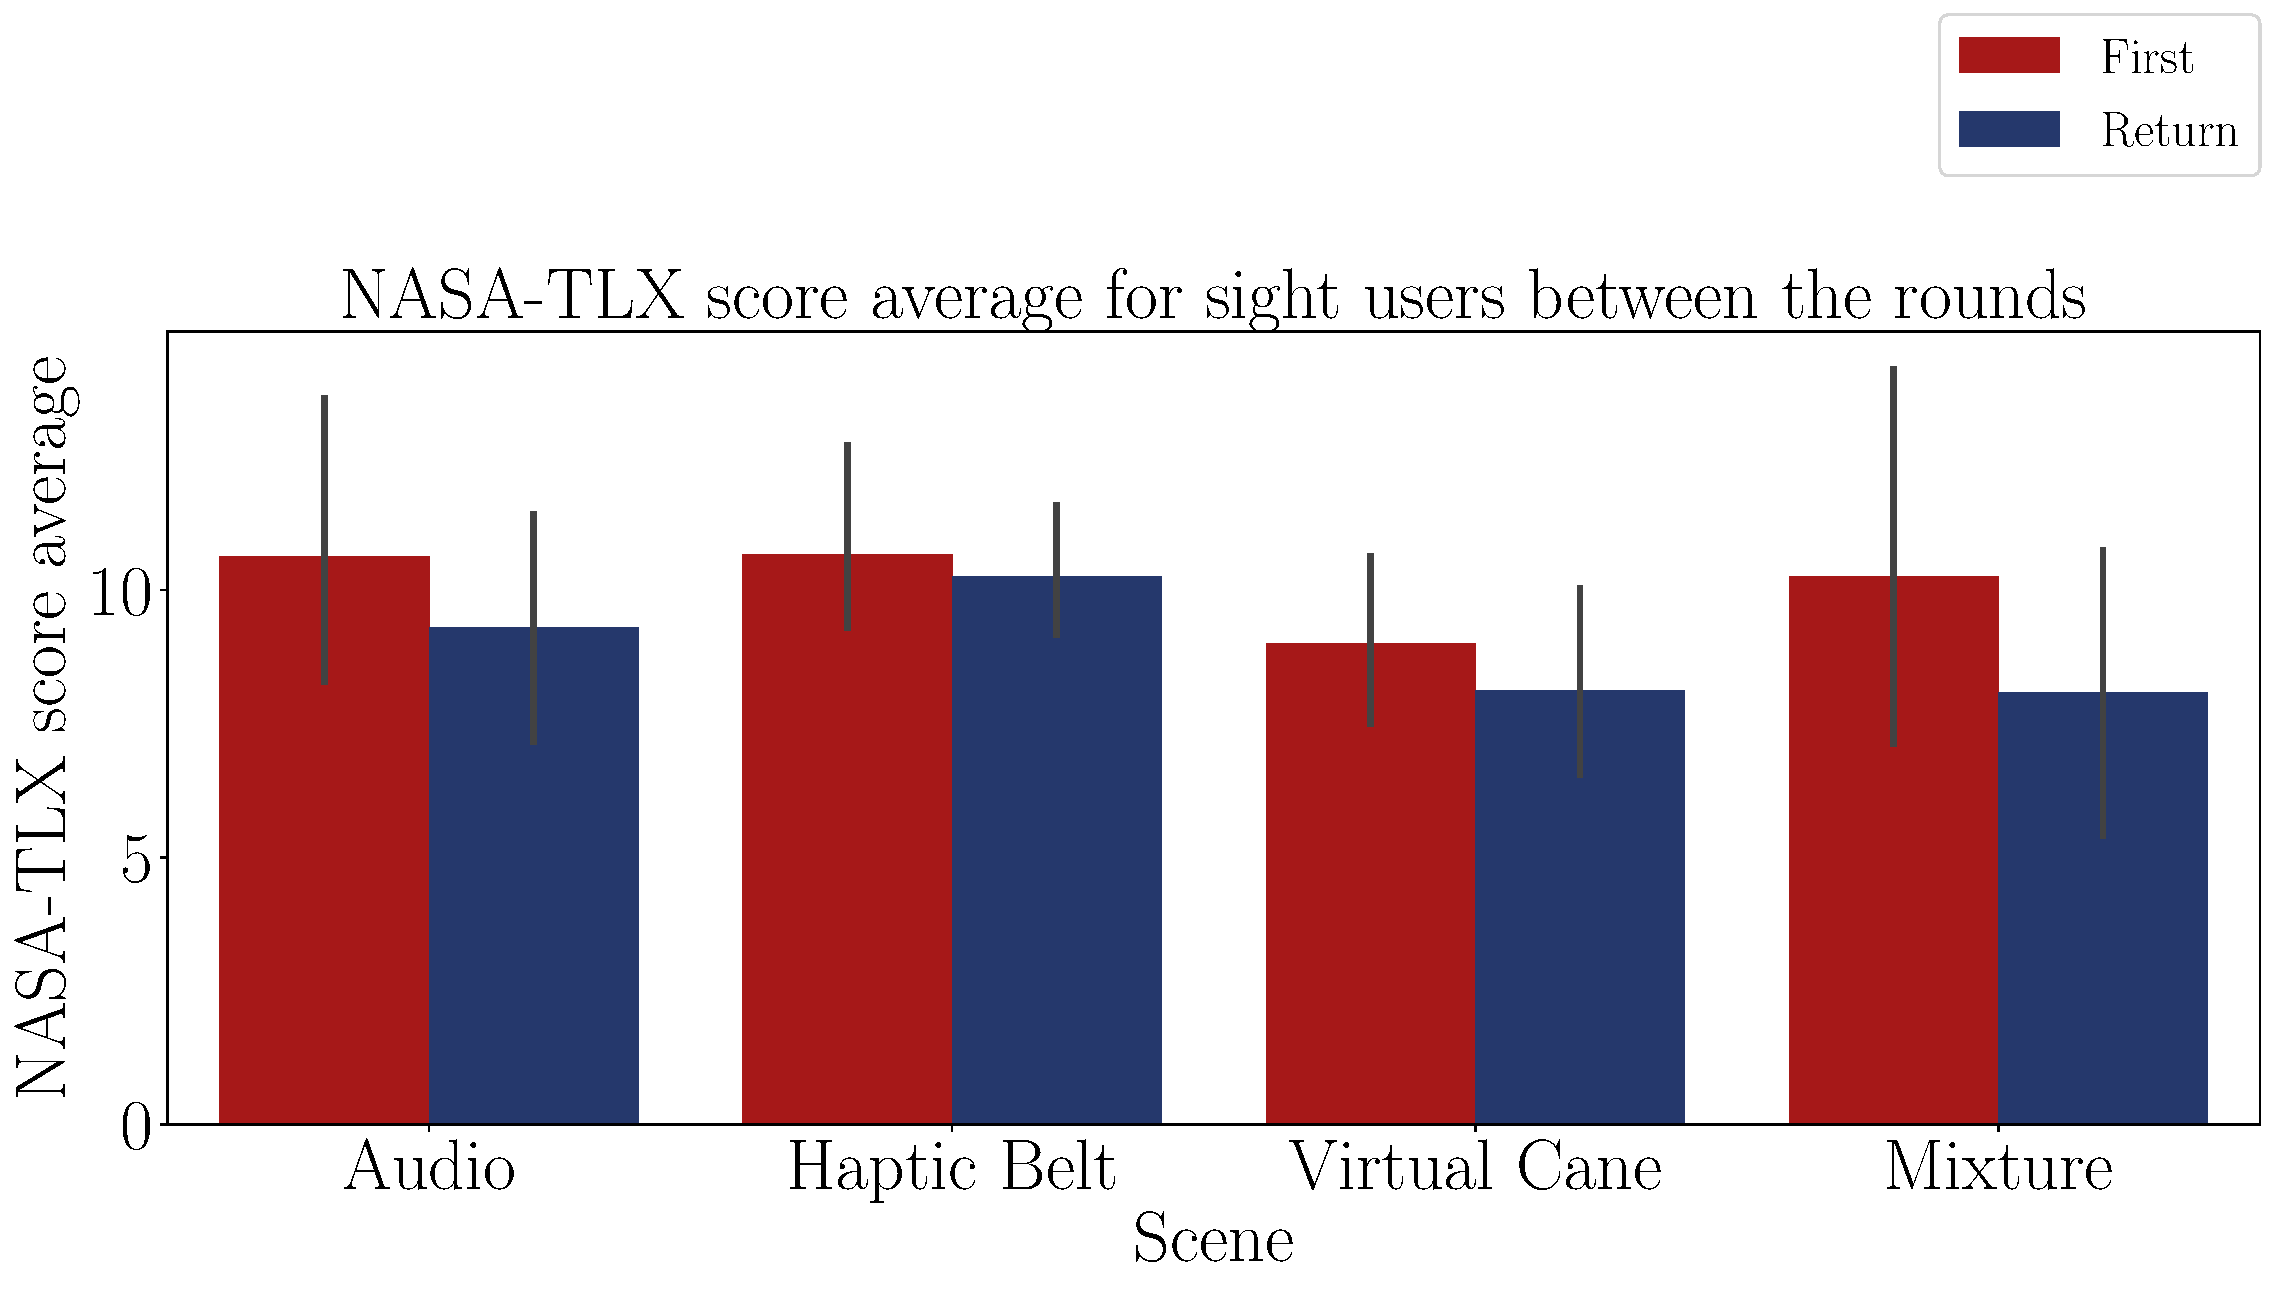
\includegraphics[width = \textwidth]{Resultados/Nasa/Figuras/pdf/barplot_nasa_avg_4_scene_sight.pdf}
        \subcaption{Sight participants.}
        \label{fig:barplot_nasa_avg_4_scene_sight}
    \end{minipage}
    \caption{Barplot of the NASA-TLX score on each method and each round.}
    \label{fig:barplot_nasa_avg_4_scene}
\end{figure}

Figures \ref{fig:boxplot_noBase_nasa_4_scene} and \ref{fig:boxplot_noBase_nasa_4_rounds} present the boxplots of the NASA-TLX global score. Again, it is possible to see that sighted people usually give higher workload scores than blind ones. The influence of the round is approximately the same. However, the order of preference of the methods is different.

\begin{figure}[!htb]
    \centering
    \begin{minipage}{0.45\textwidth}
        \centering
        \includegraphics[width = \textwidth]{Resultados/Nasa/Figuras/pdf/boxplot_noBase_nasa_4_scene.pdf}
        \caption{Boxplot of the NASA-TLX score of the participants grouped by the methods.}
        \label{fig:boxplot_noBase_nasa_4_scene}
    \end{minipage}
    \begin{minipage}{0.075\textwidth}
        \hfill
    \end{minipage}
    \begin{minipage}{0.45\textwidth}
        \centering
        \includegraphics[width = \textwidth]{Resultados/Nasa/Figuras/pdf/boxplot_noBase_nasa_4_rounds.pdf}
        \caption{Boxplot of the NASA-TLX score of the participants grouped by the rounds.}
        \label{fig:boxplot_noBase_nasa_4_rounds}
    \end{minipage}
\end{figure}

Figures \ref{fig:qqplot_nasa_avg_two_way_sight} and \ref{fig:residplot_nasa_avg_two_way_sight} bring the QQ plot and residual distribution of the data from sighted participants, showing that ANOVA can be used. The p-values for both groups are presented in Table \ref{tab:blocanova_nasa_avg_two_way_blind_sight}. It confirms the influence of the round for both sighted and blind people. In the case of the methods, the p-value of blind is lower than the threshold of 0.5, while that of sighted is slightly higher.

\begin{table}[!thb]
    \caption{Anova p-value for the NASA-TLX score on each method}
    \label{tab:blocanova_nasa_avg_two_way_blind_sight}
    \begin{minipage}{0.45\textwidth}
        \subcaption{Blind participants}
        
\centering
\begin{tabular}{ll}
\toprule
          Source & P-Value \\
\midrule
    \    Methods & 0.029** \\
     \    Rounds & 0.022** \\
\    Interaction &   0.814 \\
\bottomrule
\end{tabular}

    \end{minipage}
    \begin{minipage}{0.45\textwidth}
        \subcaption{Sight participants}
        
\centering
\begin{tabular}{ll}
\toprule
          Source & P-Value \\
\midrule
    \    Methods &   0.086 \\
     \    Rounds & 0.034** \\
\    Interaction &   0.688 \\
\bottomrule
\end{tabular}
    
    \end{minipage}
\end{table}


\begin{figure}[!htb]
    \centering
    %\vspace{-15.0cm}
    \begin{minipage}{0.45\textwidth}
        \centering
        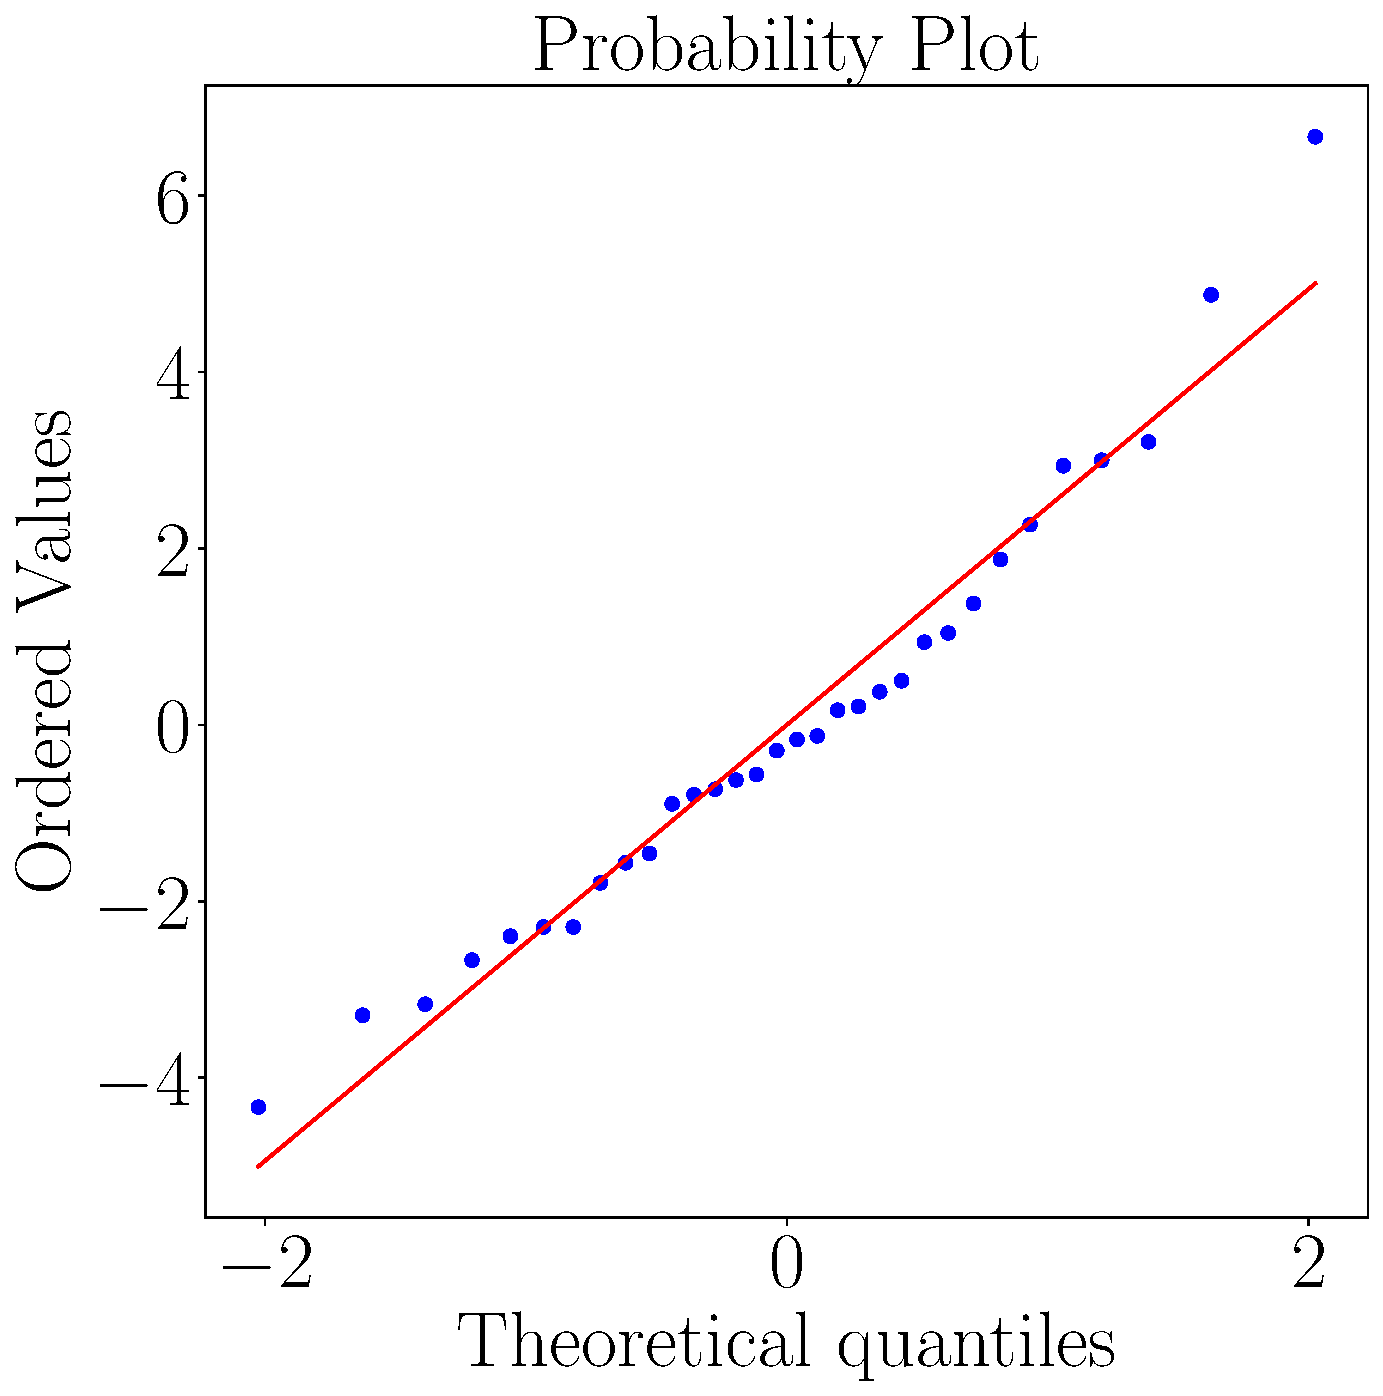
\includegraphics[width = \textwidth]{Resultados/Nasa/Figuras/pdf/qqplot_nasa_avg_two_way_sight.pdf}
        \caption{QQ plot of the NASA-TLX score of the sight participants on each method.}
        \label{fig:qqplot_nasa_avg_two_way_sight}
    \end{minipage}
    \begin{minipage}{0.075\textwidth}
        \hfill
    \end{minipage}
    \begin{minipage}{0.45\textwidth}
        \centering
        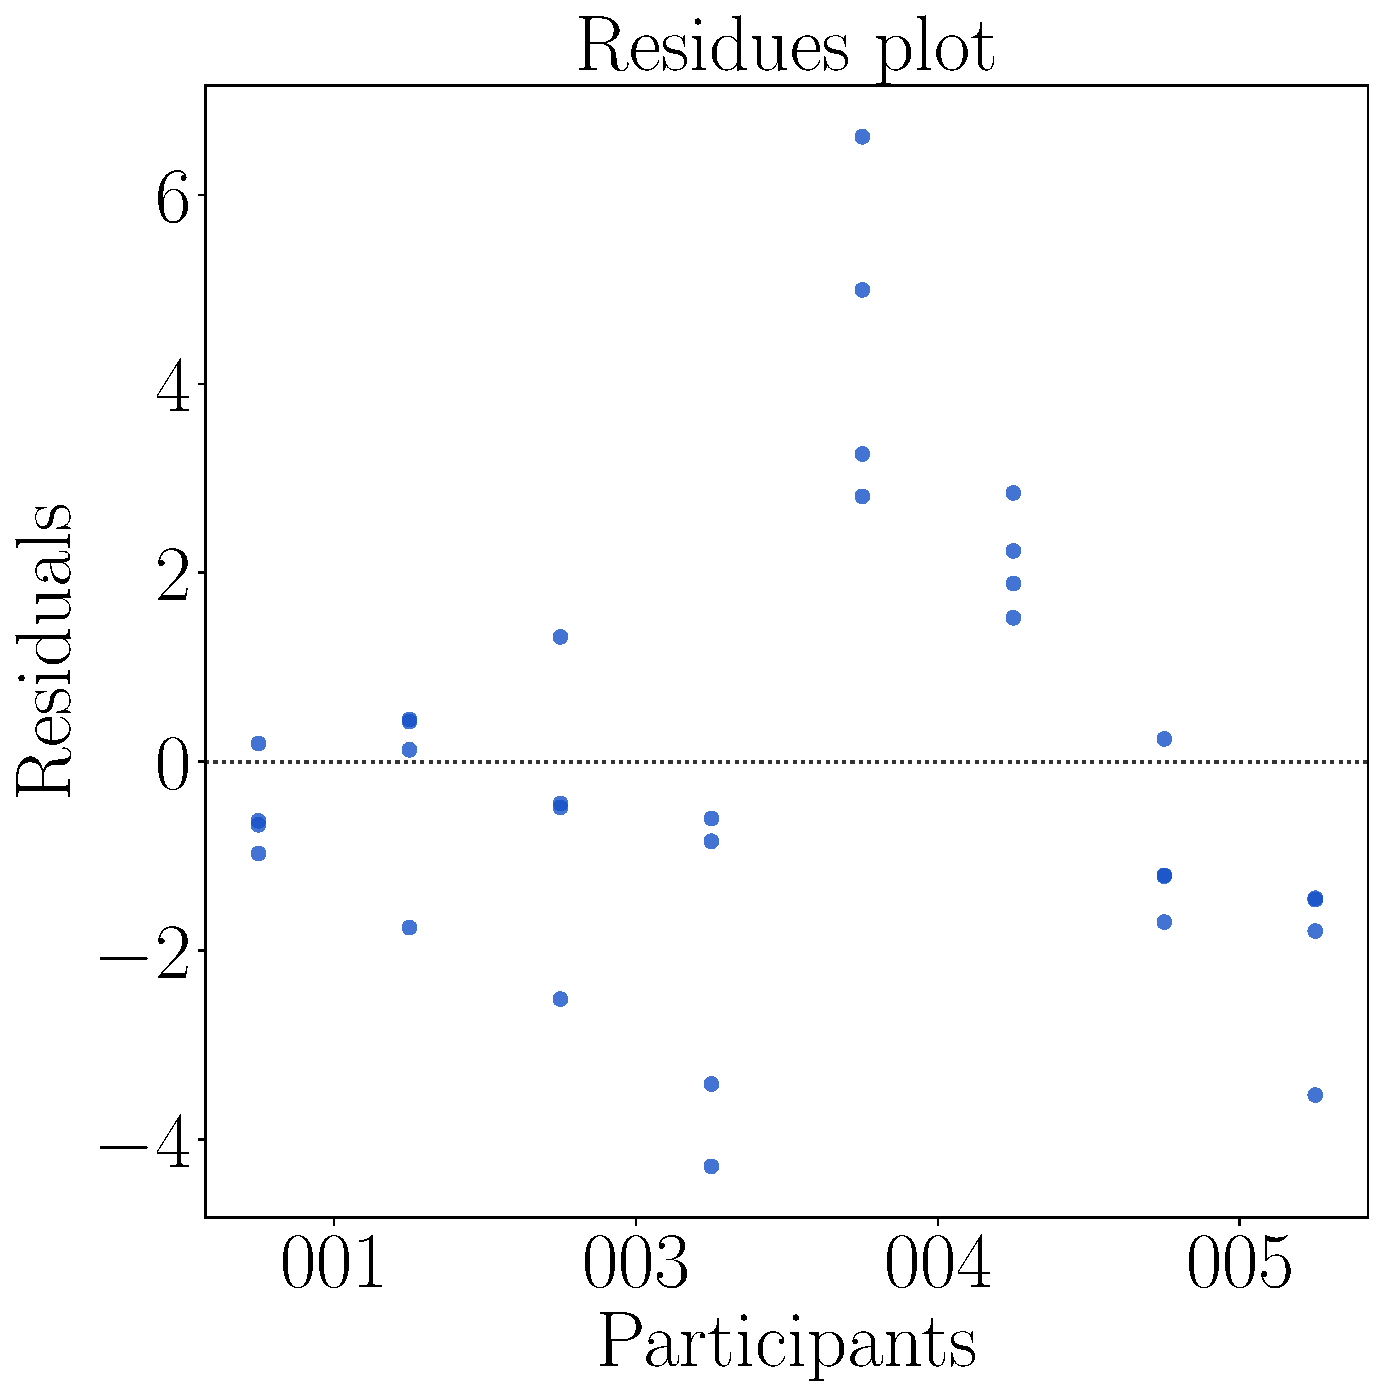
\includegraphics[width = \textwidth]{Resultados/Nasa/Figuras/pdf/residplot_nasa_avg_two_way_sight.pdf}
        \caption{Residual plot of the NASA-TLX score the sight participants on each method.}
        \label{fig:residplot_nasa_avg_two_way_sight}
    \end{minipage}
\end{figure}

\FloatBarrier

\subsubsection{Adapted SAGAT}
\label{subsubsec:results_adapted_sagat_2}

%Table \ref{tab:sagat_table_noBase} presents the SAGAT score of all participants. As said before, the higher the value, the higher is the Situation Awareness of the user. The corresponding barplot is presented in Figure \ref{fig:barplot_sagat_avg_4_scene_blind_sight}.

%
\begin{table}[!htb]
\centering
\caption{SAGAT global score felled by the participants.}
\label{tab:sagat_table_noBase}
\begin{tabular}{lllrrrrr}
\toprule
    &       &        &  Audio & \begin{tabular}[c]{@{}l@{}}Haptic\\ Belt\end{tabular} & \begin{tabular}[c]{@{}l@{}}Virtual\\ Cane\end{tabular} & Mixture \\
Participant & \begin{tabular}[c]{@{}l@{}}Visual\\ Condition\end{tabular} & Round &        &                                                       &                                                        &         \\
\midrule
001C & Blind & First &  5.500 &                                                 5.330 &                                                  5.830 &   3.500 \\
    &       & Return &  6.500 &                                                 8.500 &                                                  5.500 &   5.500 \\
002C & Blind & First &  4.500 &                                                 3.990 &                                                  4.500 &   6.250 \\
    &       & Return &  5.000 &                                                 4.000 &                                                  6.500 &   8.500 \\
003C & Blind & First &  7.500 &                                                 7.490 &                                                  4.660 &   9.000 \\
    &       & Return & 10.000 &                                                 8.500 &                                                  9.000 &   9.000 \\
004C & Blind & First &  6.000 &                                                 7.660 &                                                  4.990 &   6.500 \\
    &       & Return &  6.000 &                                                 9.250 &                                                  7.250 &   9.000 \\
001 & Sight & First &  4.500 &                                                 4.330 &                                                  2.660 &   6.500 \\
    &       & Return &  6.000 &                                                 5.000 &                                                  5.000 &   4.500 \\
003 & Sight & First &  6.750 &                                                 5.990 &                                                  3.990 &   6.750 \\
    &       & Return &  6.000 &                                                 7.250 &                                                  6.250 &   7.500 \\
004 & Sight & First &  7.250 &                                                 7.990 &                                                  5.990 &   8.250 \\
    &       & Return &  7.750 &                                                 9.500 &                                                  8.250 &   7.000 \\
005 & Sight & First &  3.000 &                                                 3.160 &                                                  3.990 &   4.000 \\
    &       & Return &  3.750 &                                                 3.000 &                                                  2.000 &   6.000 \\
\bottomrule
\end{tabular}
\end{table}



%Figure \ref{fig:barplot_sagat_avg_4_scene_blind_sight}. shows that the SAGAT score for sighted participants is, on average lower than that of blind participants, which is expected as they are not used to navigating without vision. Also, the increase in situation awareness from the first to the return round is lower. In the case of the mixture method, the SAGAT score did not improve at all. For both groups, the virtual cane was the method with the lowest score in the first round.
%
%\begin{figure}[!htb]
%    \centering
%    \begin{minipage}{\linewidth}
%        \centering
%        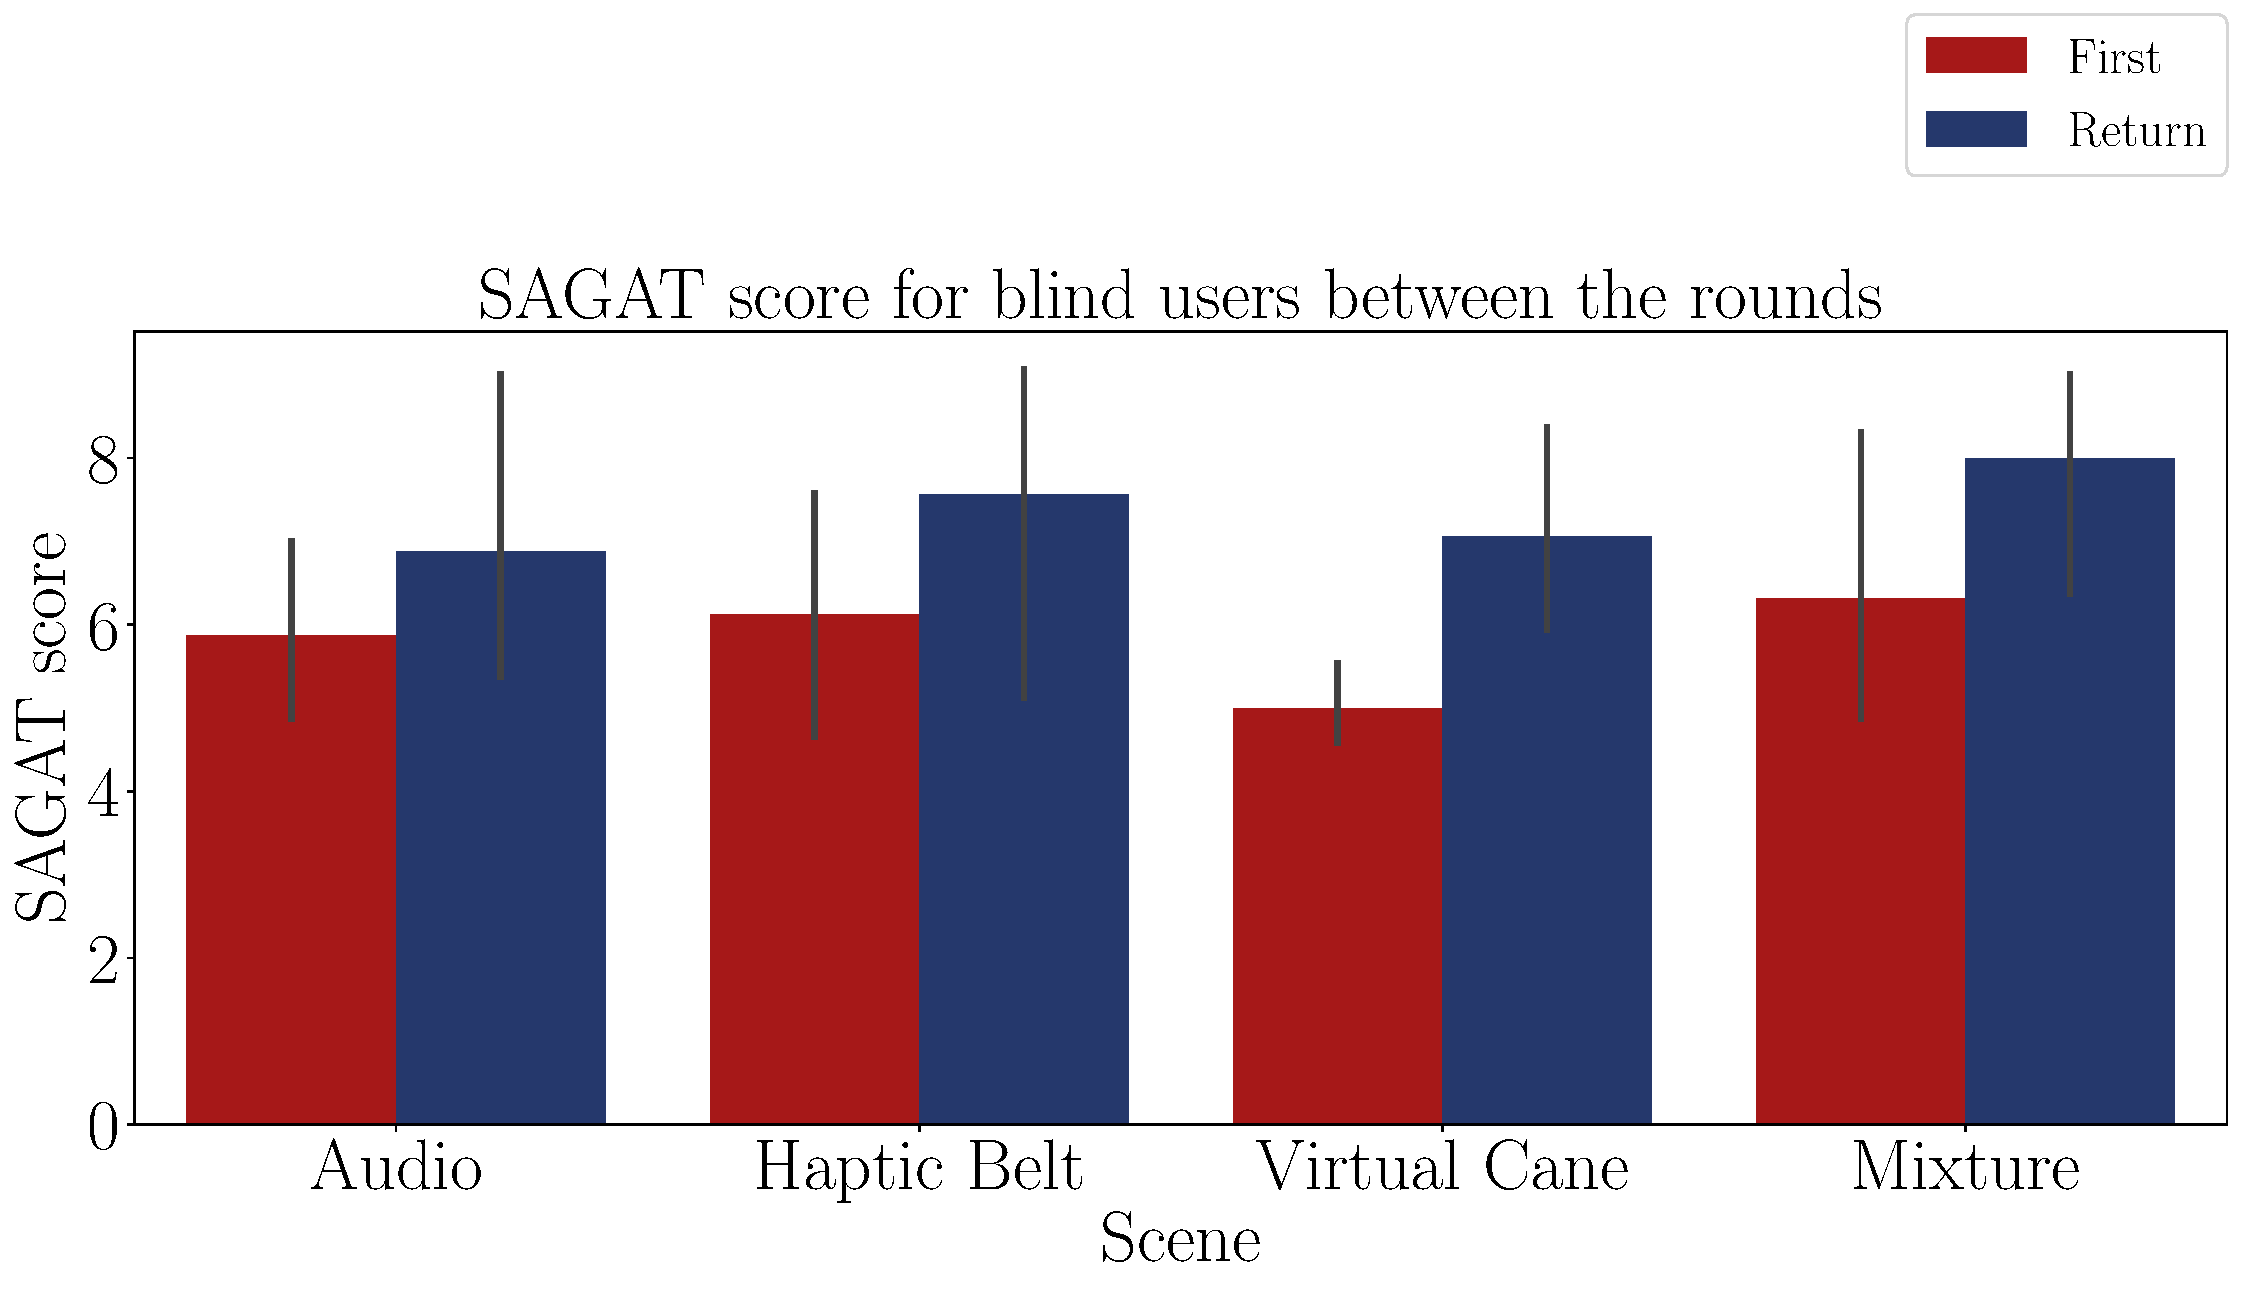
\includegraphics[width = \linewidth]{Resultados/Sagat/Figuras/pdf/barplot_sagat_avg_4_scene_blind.pdf}
%        \subcaption{Blind participants.}
%        \label{fig:barplot_sagat_avg_4_scene_blind}
%    \end{minipage}
%    \begin{minipage}{\linewidth}
%        \centering
%        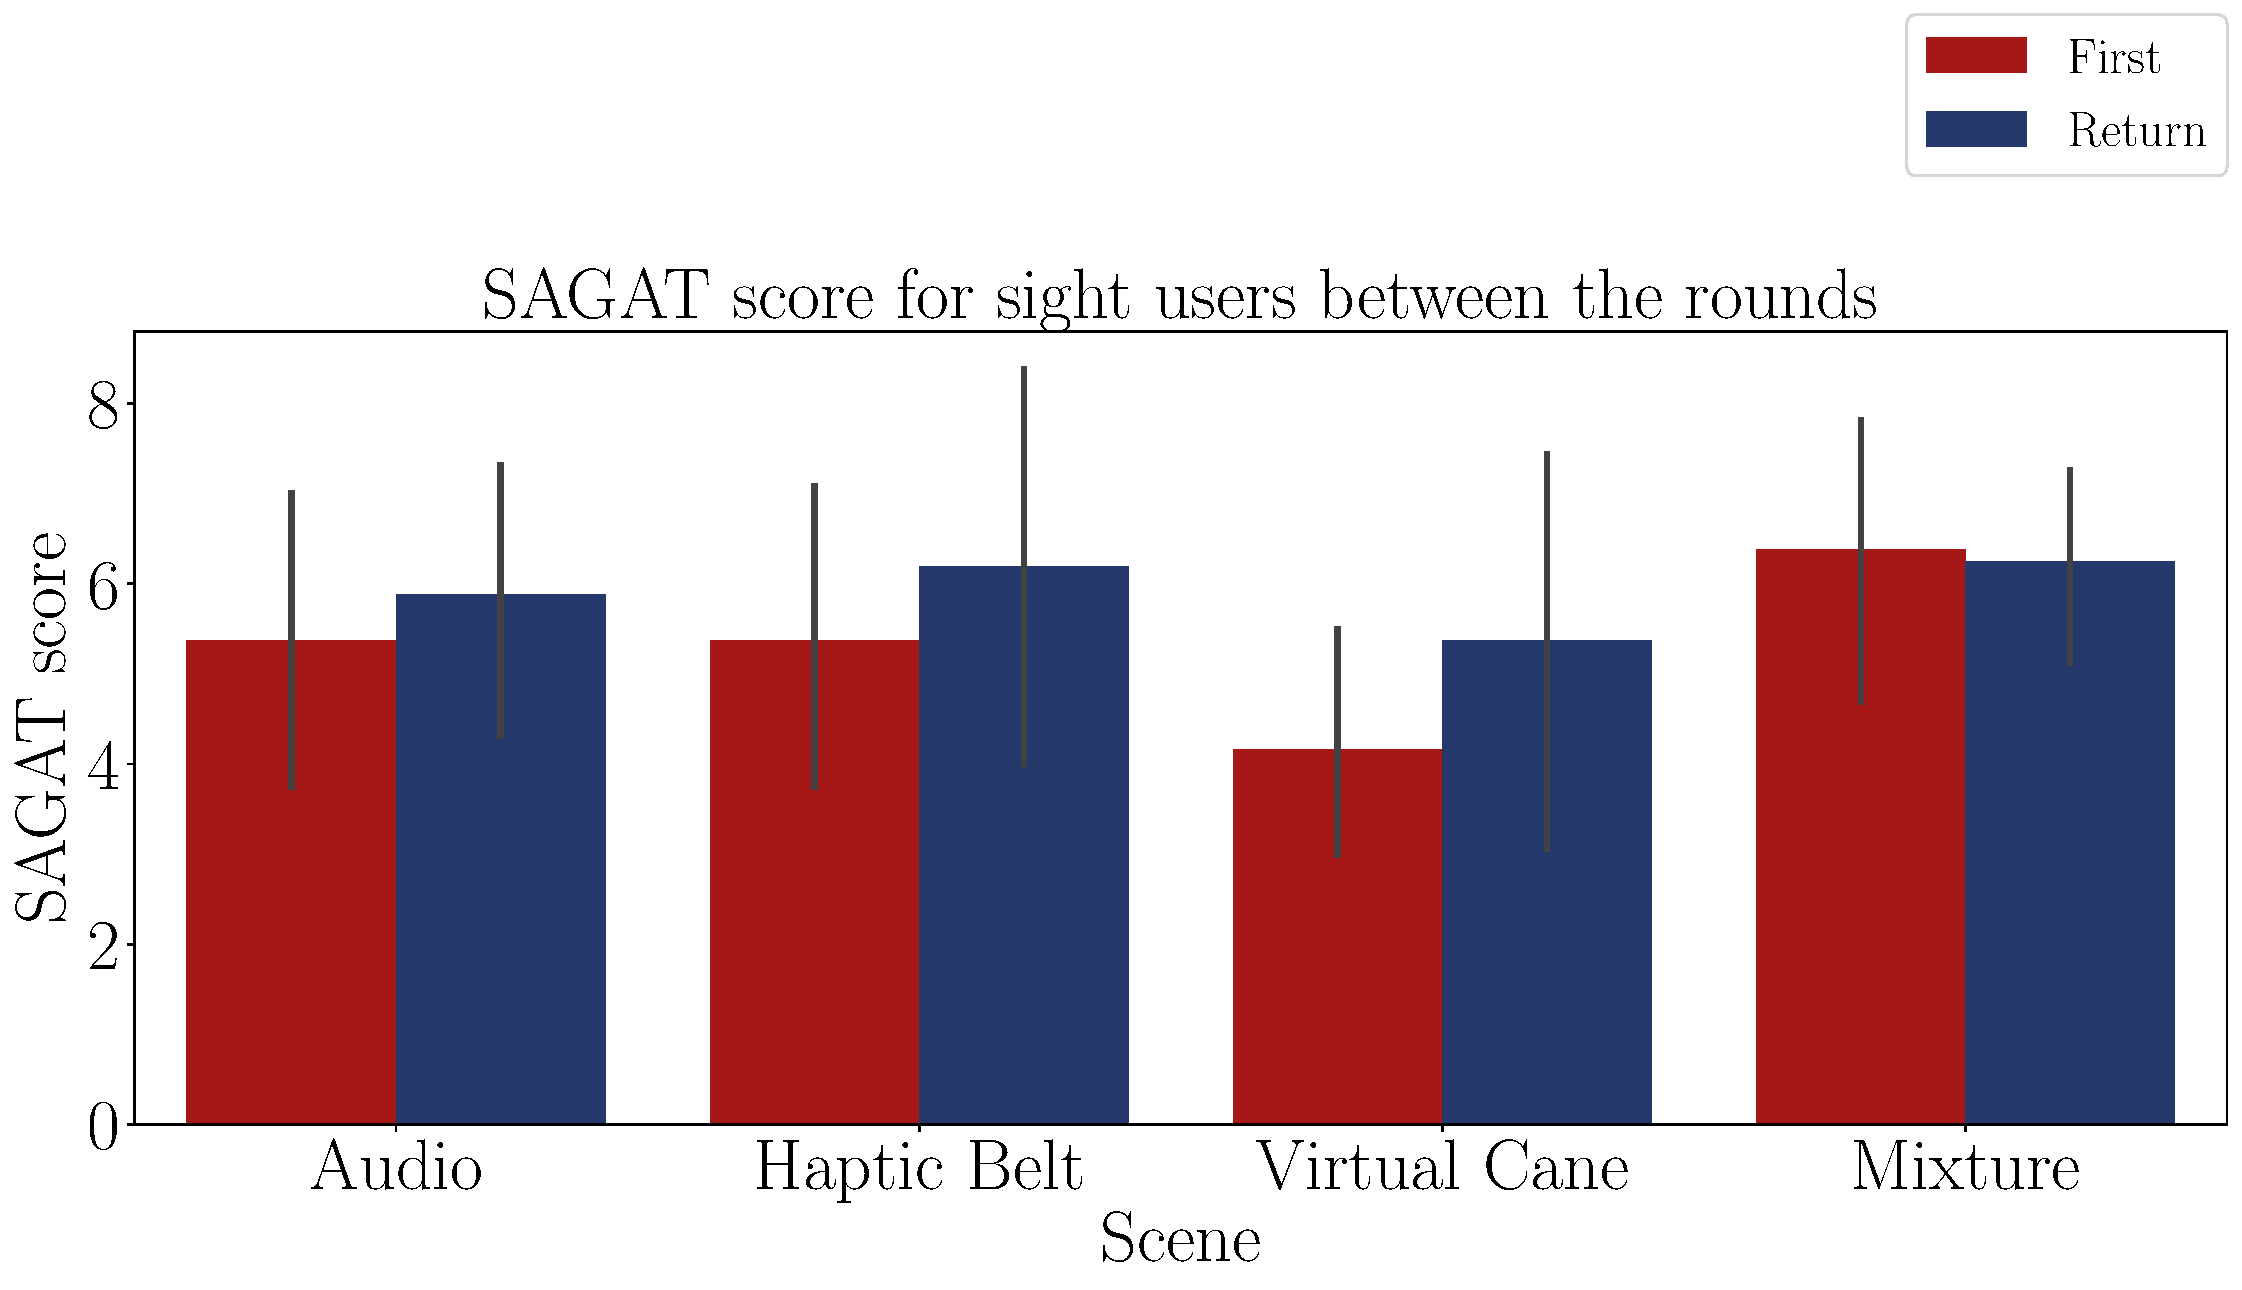
\includegraphics[width = \linewidth]{Resultados/Sagat/Figuras/pdf/barplot_sagat_avg_4_scene_sight.pdf}
%        \subcaption{Sight participants.}
%        \label{fig:barplot_sagat_avg_4_scene_sight}
%    \end{minipage}
%    \caption{Barplot of the SAGAT score on each method and each round.}
%    \label{fig:barplot_sagat_avg_4_scene_blind_sight}
%\end{figure}

Figures \ref{fig:boxplot_sagat_4_scene} and \ref{fig:boxplot_sagat_4_rounds} bring the boxplots. According to Figure \ref{fig:boxplot_sagat_4_scene}, both groups presented a higher situation awareness with ‘mixture’ and ‘haptic’. On the other hand, Figure \ref{fig:boxplot_sagat_4_rounds} confirms that the difference between the rounds is more significant for blind participants. 

\begin{figure}[!htb]
    \centering
    \includegraphics[width = 0.75\linewidth]{Resultados/Sagat/Figuras/pdf/boxplot_sagat_4_scene.pdf}
    \caption{Boxplot of the Sagat score of the participants grouped by the methods.}
    \label{fig:boxplot_sagat_4_scene}
\end{figure}
\begin{figure}[!htb]
    \centering
    \includegraphics[width = 0.75\linewidth]{Resultados/Sagat/Figuras/pdf/boxplot_sagat_4_rounds.pdf}
    \caption{Boxplot of the Sagat score of the participants grouped by the rounds.}
    \label{fig:boxplot_sagat_4_rounds}
\end{figure}

%Figures \ref{fig:qqplot_sagat_avg_two_way_sight} and \ref{fig:residplot_sagat_avg_two_way_sight} brings the QQ plot and residual distribution. 
The variance of the residuals is not equal among the participants. Table \ref{tab:blocanova_sagat_avg_two_way_blind_sight} brings the p-value from ANOVA. While for the blind participants, the rounds are a significant factor and the methods are not, for the sighted participants the result is the opposite, showing a significant influence of the methods and not of the rounds.

\begin{table}[!htb]
    \caption{Anova p-value for the SAGAT score on each method}
    \label{tab:blocanova_sagat_avg_two_way_blind_sight}
\begin{minipage}{0.45\linewidth}
    \subcaption{Blind participants}
    
\centering
\begin{tabular}{ll}
\toprule
          Source & P-Value \\
\midrule
    \    Methods &   0.277 \\
     \    Rounds & 0.002** \\
\    Interaction &   0.834 \\
\bottomrule
\end{tabular}

\end{minipage}%
\begin{minipage}{0.05\linewidth}
    \hfill
\end{minipage}%
\begin{minipage}{0.45\linewidth}
    \subcaption{Sight participants}
    
\centering
\begin{tabular}{ll}
\toprule
          Source & P-Value \\
\midrule
    \    Methods & 0.035** \\
     \    Rounds &   0.095 \\
\    Interaction &   0.578 \\
\bottomrule
\end{tabular}
    
\end{minipage}
\end{table}


%\begin{figure}[!htb]
%    \centering
%    %\vspace{-15.0cm}
%    \begin{minipage}{0.45\linewidth}
%        \centering
%        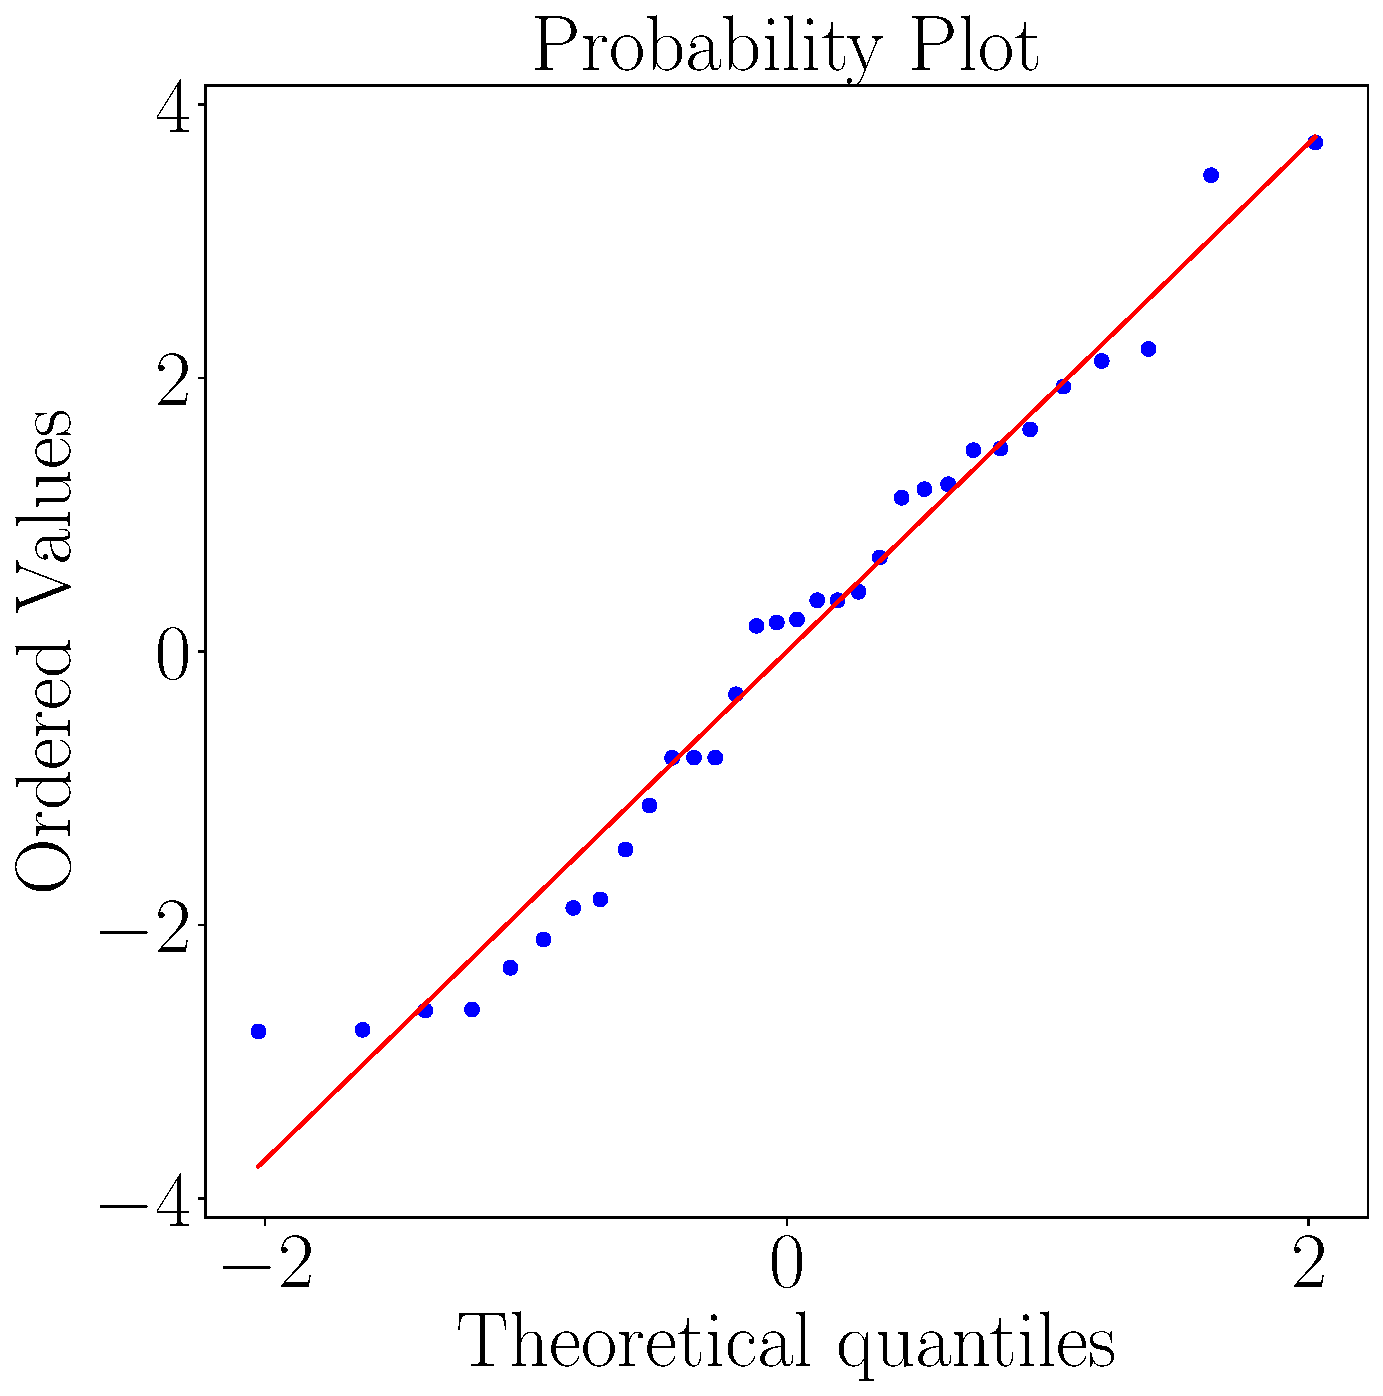
\includegraphics[width = \linewidth]{Resultados/Sagat/Figuras/pdf/qqplot_sagat_avg_two_way_sight.pdf}
%        \caption{QQ plot of the mental demand of the sight participants on each method.}
%        \label{fig:qqplot_sagat_avg_two_way_sight}
%    \end{minipage}
%    \begin{minipage}{0.075\linewidth}
%        \hfill
%    \end{minipage}
%    \begin{minipage}{0.45\linewidth}
%        \centering
%        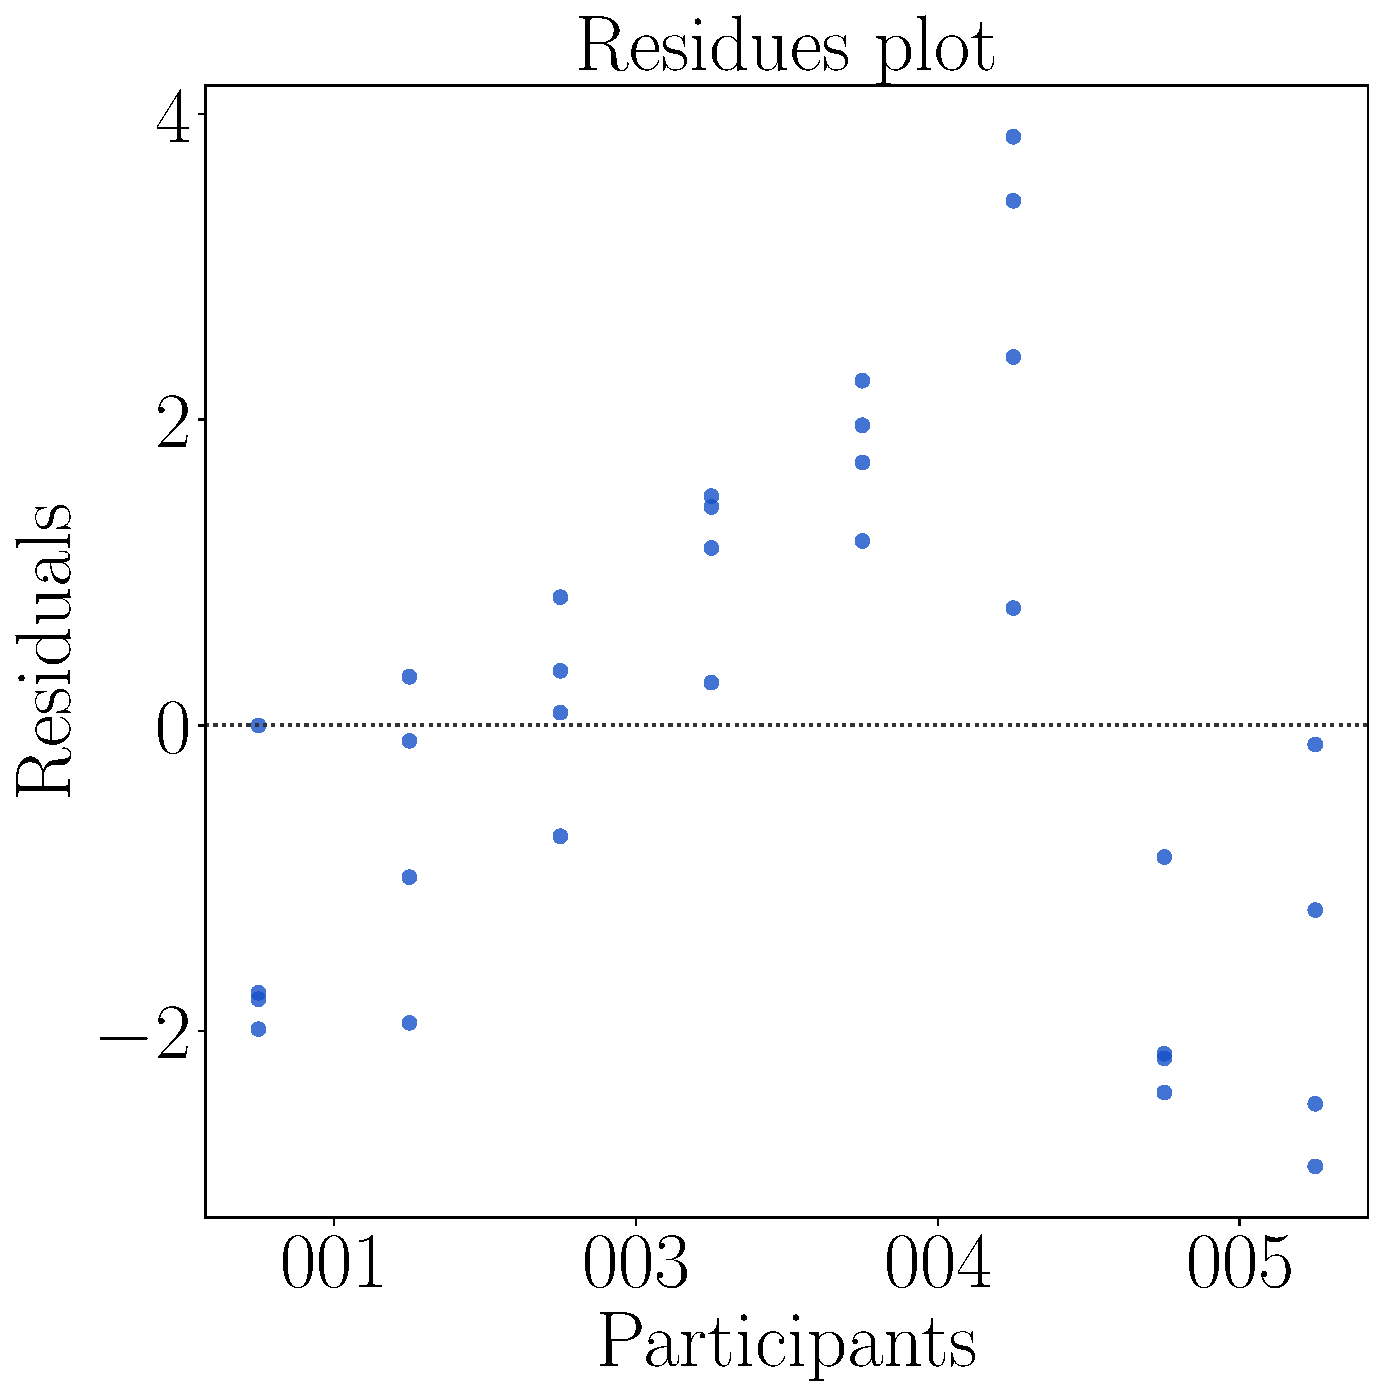
\includegraphics[width = \linewidth]{Resultados/Sagat/Figuras/pdf/residplot_sagat_avg_two_way_sight.pdf}
%        \caption{Residual plot of the mental demand score the sight participants on each method.}
%        \label{fig:residplot_sagat_avg_two_way_sight}
%    \end{minipage}
%\end{figure}
%
%%%%%%%%%%%%%%%%%%%%%%%%%%%%%%%%%%%%%%%%%%%%%%%%%%%%%%
%
%\FloatBarrier

\subsubsection{Guidance method's questionnaire.}
\label{subsubsec:results_questionnaires_2}

%As for the blind users, the sighted user also answered the Guidance questionnaire to give their thoughts about their experience with the guidance methods. Table \ref{tab:questionnaire_average} shows the score of both groups. As said before, the higher the value, the higher is the user satisfaction. The corresponding barplots are presented in Figure \ref{fig:barplot_questionnaire_scene_blind_sight}. Both groups prefer audio  and mixture methods. The difference lies in the preference between the haptic belt and virtual cane. The blind users tend to prefer the first one, while the sighted users tend to prefer the last.

%
\begin{table}[!htb]
\centering
\caption{Guidance method questionnaire score grouped by participant.}
\label{tab:questionnaire_average}
\begin{tabular}{lllrrrrr}
\toprule
{} & Audio & \begin{tabular}[c]{@{}l@{}}Haptic\\ Belt\end{tabular} & \begin{tabular}[c]{@{}l@{}}Virtual\\ Cane\end{tabular} & Mixture & Visual Condition \\
Participant &       &                                                       &                                                        &         &                  \\
\midrule
001C        &  0.77 &                                                  0.54 &                                                   0.63 &    0.87 &            Blind \\
002C        &  0.86 &                                                  0.74 &                                                   0.54 &    0.93 &            Blind \\
003C        &  0.93 &                                                  0.57 &                                                   0.54 &    0.74 &            Blind \\
004C        &  0.88 &                                                  0.49 &                                                   0.40 &    0.73 &            Blind \\
001         &  0.75 &                                                  0.49 &                                                   0.57 &    0.69 &            Sight \\
003         &  0.76 &                                                  0.54 &                                                   0.54 &    0.78 &            Sight \\
004         &  0.86 &                                                  0.60 &                                                   0.79 &    0.76 &            Sight \\
005         &  0.61 &                                                  0.57 &                                                   0.75 &    0.84 &            Sight \\
\bottomrule
\end{tabular}
\end{table}



%\begin{figure}[!htb]
%    \centering
%    \begin{minipage}{\textwidth}
%        \centering
%        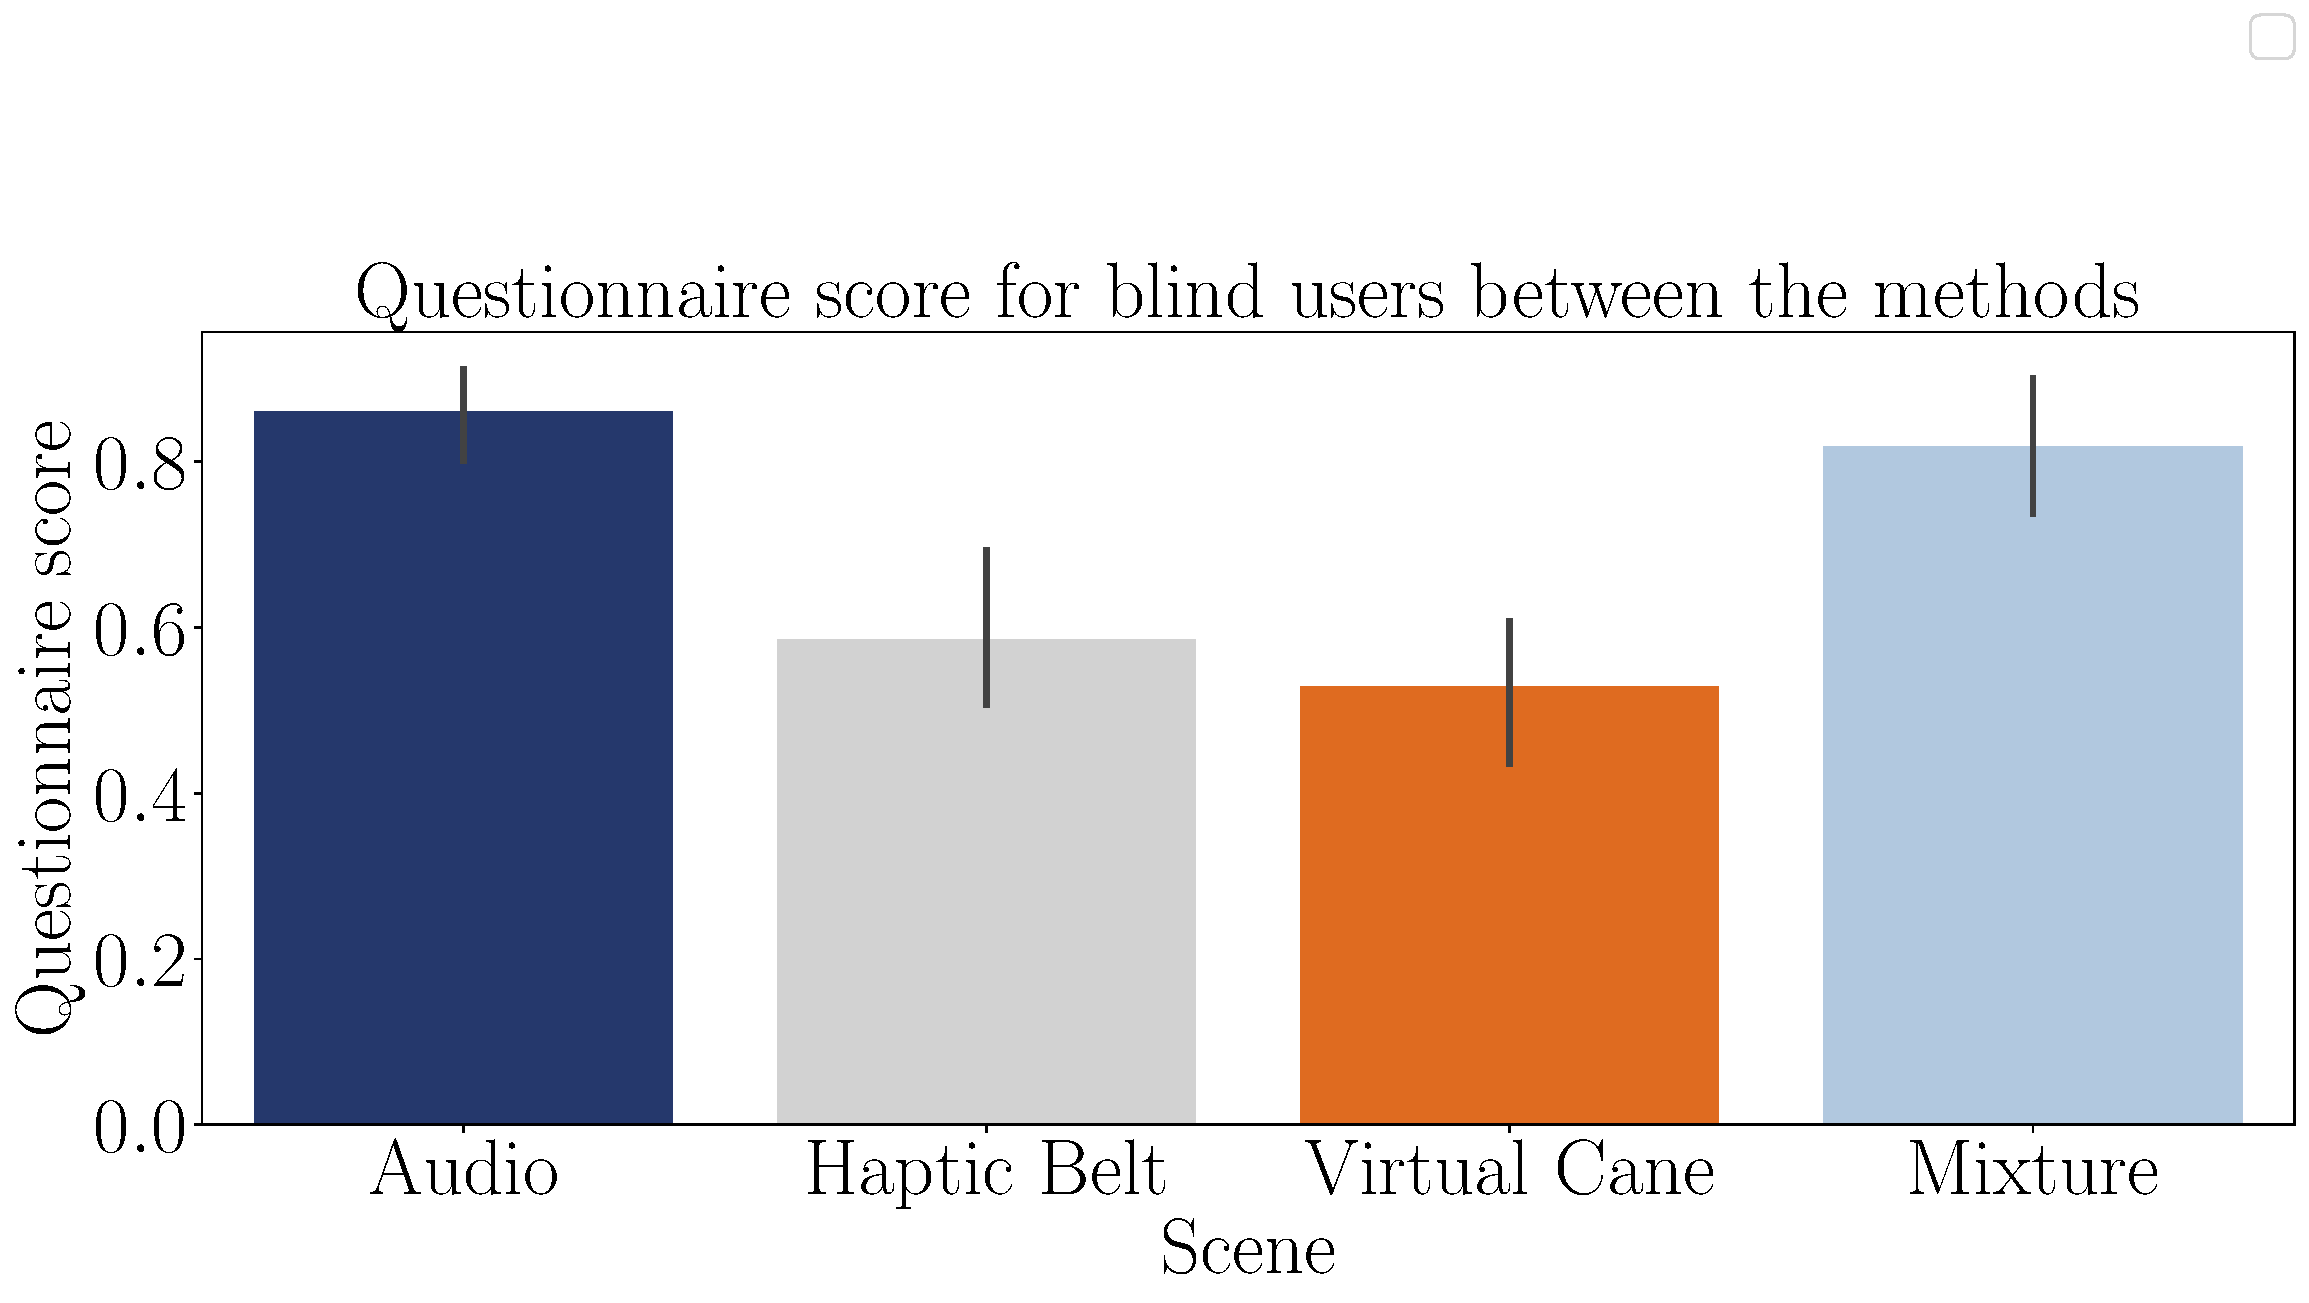
\includegraphics[width = \textwidth]{Resultados/Questionario/Figuras/pdf/barplot_questionnaire_scene_blind.pdf}
%        \subcaption{Blind participants.}
%        \label{fig:barplot_questionnaire_scene_blind_2}
%    \end{minipage}
%    \begin{minipage}{\textwidth}
%        \centering
%        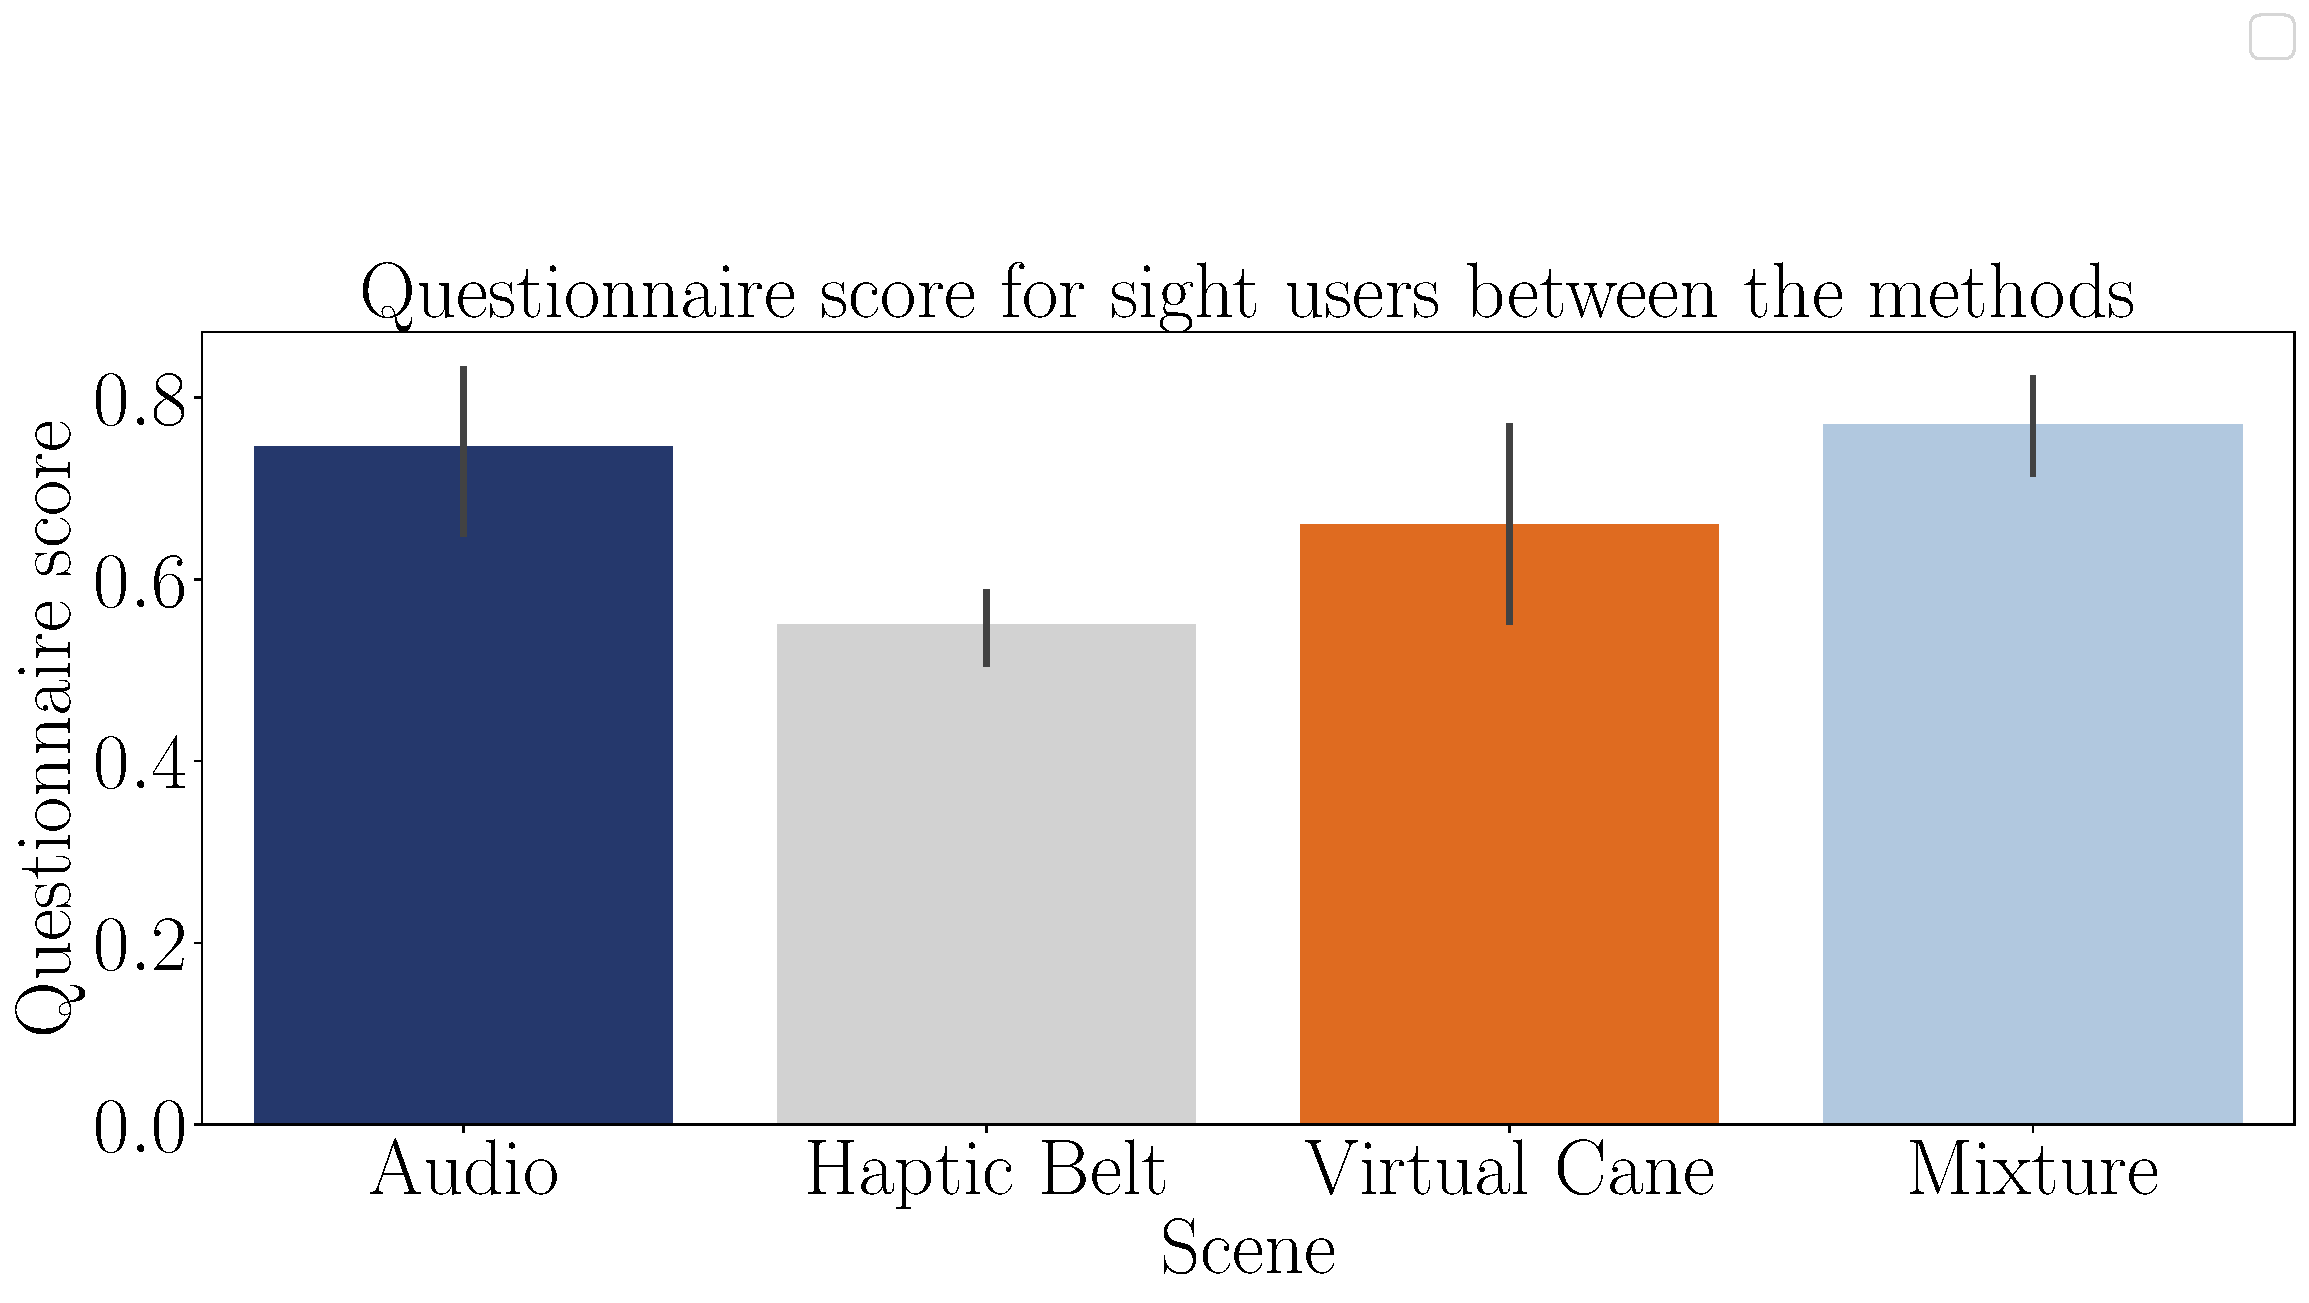
\includegraphics[width = \textwidth]{Resultados/Questionario/Figuras/pdf/barplot_questionnaire_scene_sight.pdf}
%        \subcaption{Sighted participants.}
%        \label{fig:barplot_questionnaire_scene_sight}
%    \end{minipage}
%    \caption{Barplot of the average questionaire score on each method.}
%    \label{fig:barplot_questionnaire_scene_blind_sight}
%\end{figure}
%\begin{figure}[!htb]
%    \centering
%    \includegraphics[width = \textwidth]{Resultados/Questionario/Figuras/png/barplot_questionnaire_scene.png}
%    \caption{Barplot of the  average questionaire score of both participants on each method.}
%    \label{fig:barplot_questionnaire_scene}
%\end{figure}

The Figure \ref{fig:boxplot_questionnaire_scene} presents the box plot with the distribution of the scores. It is possible to see that there is some similarity between the two groups, except for the virtual cane method, which has a broader distribution for the sighted users. Also, it seems that the audio and mixture have similar acceptance for sighted and blind users.

\begin{figure}[!htb]
    \centering
    \includegraphics[width = 0.75\linewidth]{Resultados/Questionario/Figuras/pdf/boxplot_questionnaire_scene.pdf}
    \caption{Boxplot of the questionaire score of the the participants grouped by the methods.}
    \label{fig:boxplot_questionnaire_scene}
\end{figure}

%The Table \ref{tab:questionnaire_average_group} show the the average questionnaire score on each method of both groups and it shows the same conclusion as the Figure \ref{fig:barplot_questionnaire_scene}, that the preference between the "Haptic Belt" and "Virtual Cane" is the only difference between the two groups.
%
%Considering the most preferable and the less preferable of each group, the blind users are score their choices more intesiver than the sighted users. This may be an effect from their previous experience with the "Audio" method in previous events before the experiment and with haptic devices were something very, or almost, new. For the sighted users everything was new, so there scores were more consistent. This is posible to see in the average and standar deviation of these scores. For the blind users is 0.7 and 0.164 and for the sighted user is 0.682 and 0.100.
%
%
\begin{table}[!htb]
\centering
\caption{Guidance method questionnaire average score grouped by visual condition.}
\label{tab:questionnaire_average_group}
\begin{tabular}{lrrrrr}
\toprule
{} & Audio & Haptic Belt & Virtual Cane & Mixture \\
Visual Condition &       &             &              &         \\
\midrule
Blind            &  0.86 &        0.59 &         0.53 &    0.82 \\
Sight            &  0.75 &        0.55 &         0.66 &    0.77 \\
\bottomrule
\end{tabular}
\end{table}



%Figures \ref{fig:qqplot_questionnaire_sight} and \ref{fig:residplot_questionnaire_sight} brings the QQ plot and residual distribution, which confirm that ANOVA can be applied.
The result of ANOVA is presented in Table \ref{tab:blocanova_questionnaire_blind_sight} and indicates that the method is an effective variable for the sighted participants, as it is for the blind ones.

\begin{table}[!htb]
    \caption{Anova p-value for the questionnaire score on each method}
    \label{tab:blocanova_questionnaire_blind_sight}
\begin{minipage}{0.45\linewidth}
    \subcaption{Blind participants.}
    
\centering
\begin{tabular}{ll}
\toprule
Source & P-Value \\
\midrule
Method & 0.001** \\
\bottomrule
\end{tabular}

\end{minipage}%
\begin{minipage}{0.05\linewidth}
\end{minipage}%
\begin{minipage}{0.45\linewidth}
    \subcaption{Sight participants.}
    
\centering
\begin{tabular}{ll}
\toprule
Source & P-Value \\
\midrule
Method & 0.016** \\
\bottomrule
\end{tabular}

\end{minipage}
\end{table}

%\begin{figure}[!htb]
%    \centering
%    %\vspace{-15.0cm}
%    \begin{minipage}{0.45\textwidth}
%        \centering
%        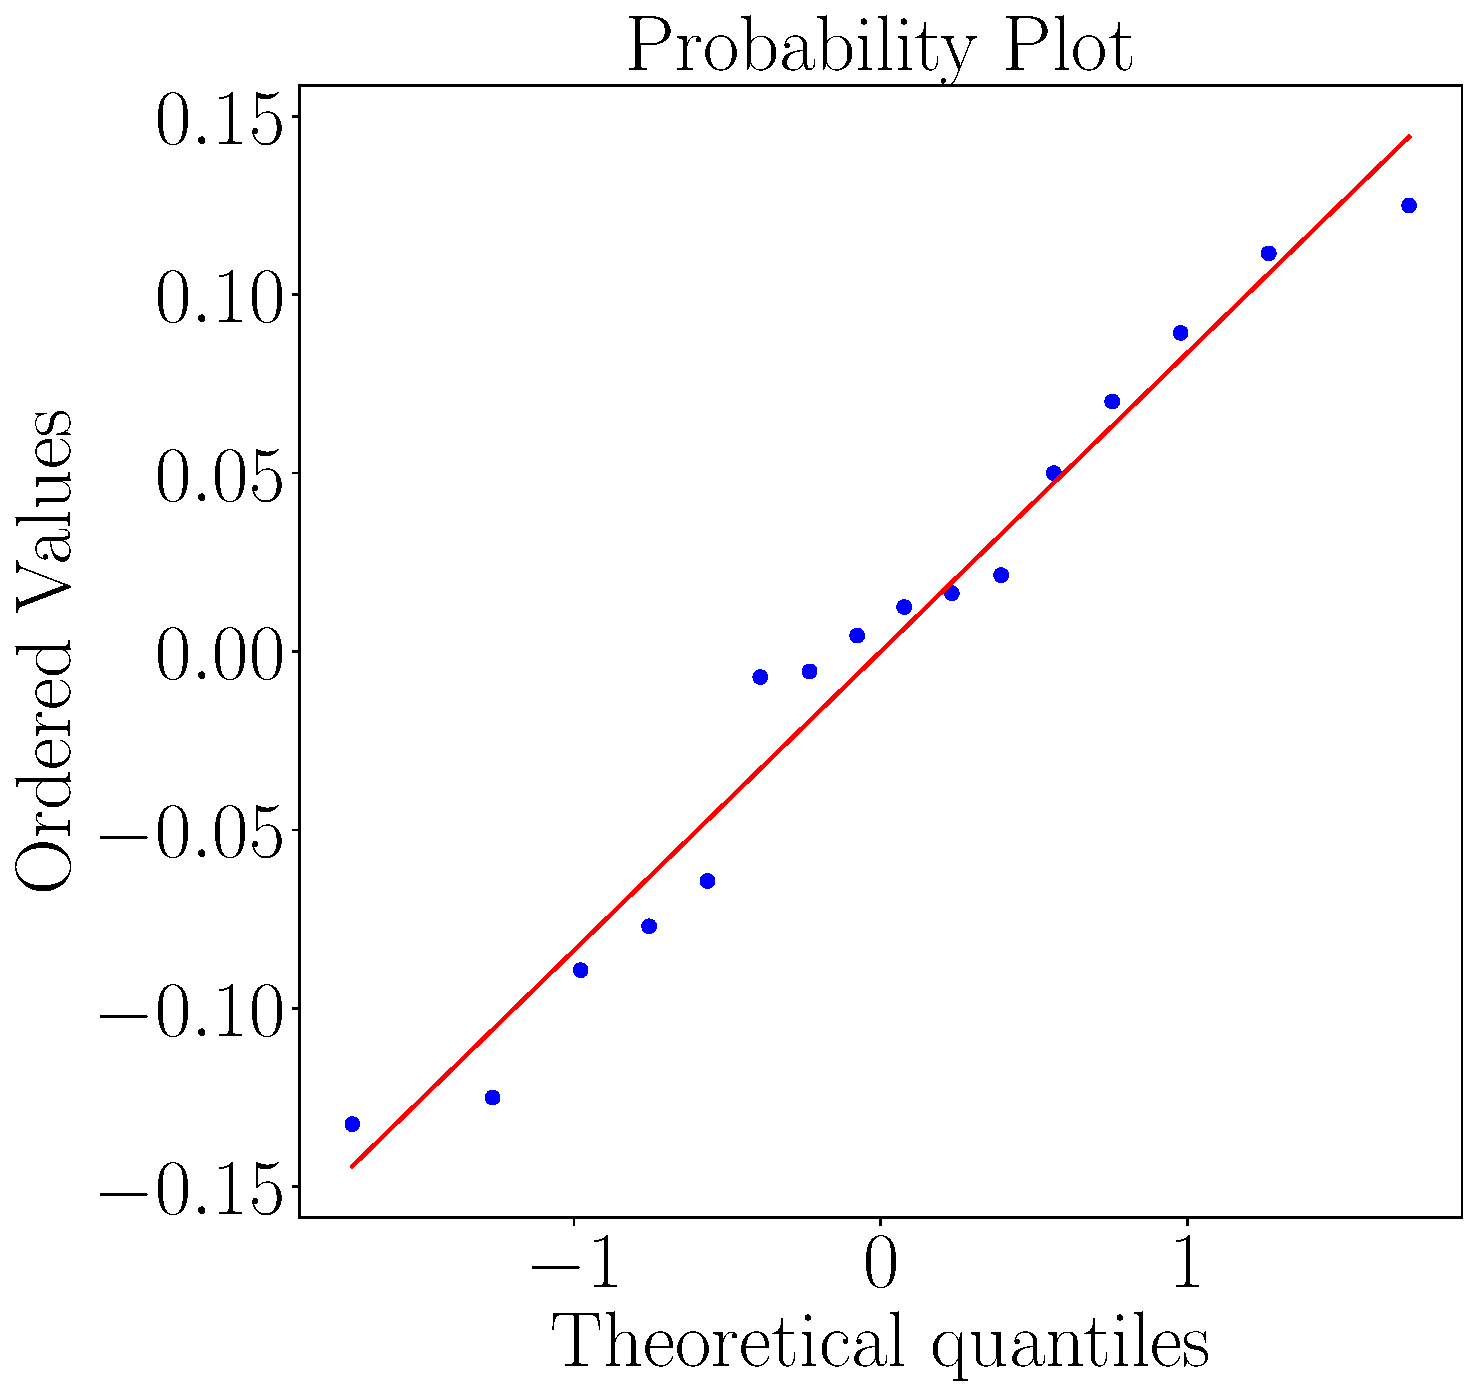
\includegraphics[width = \textwidth]{Resultados/Questionario/Figuras/pdf/qqplot_questionnaire_sight.pdf}
%        \caption{QQ plot of the questionnaire score of the sighted participants on each method.}
%        \label{fig:qqplot_questionnaire_sight}
%    \end{minipage}
%    \begin{minipage}{0.075\textwidth}
%        \hfill
%    \end{minipage}
%    \begin{minipage}{0.45\textwidth}
%        \centering
%        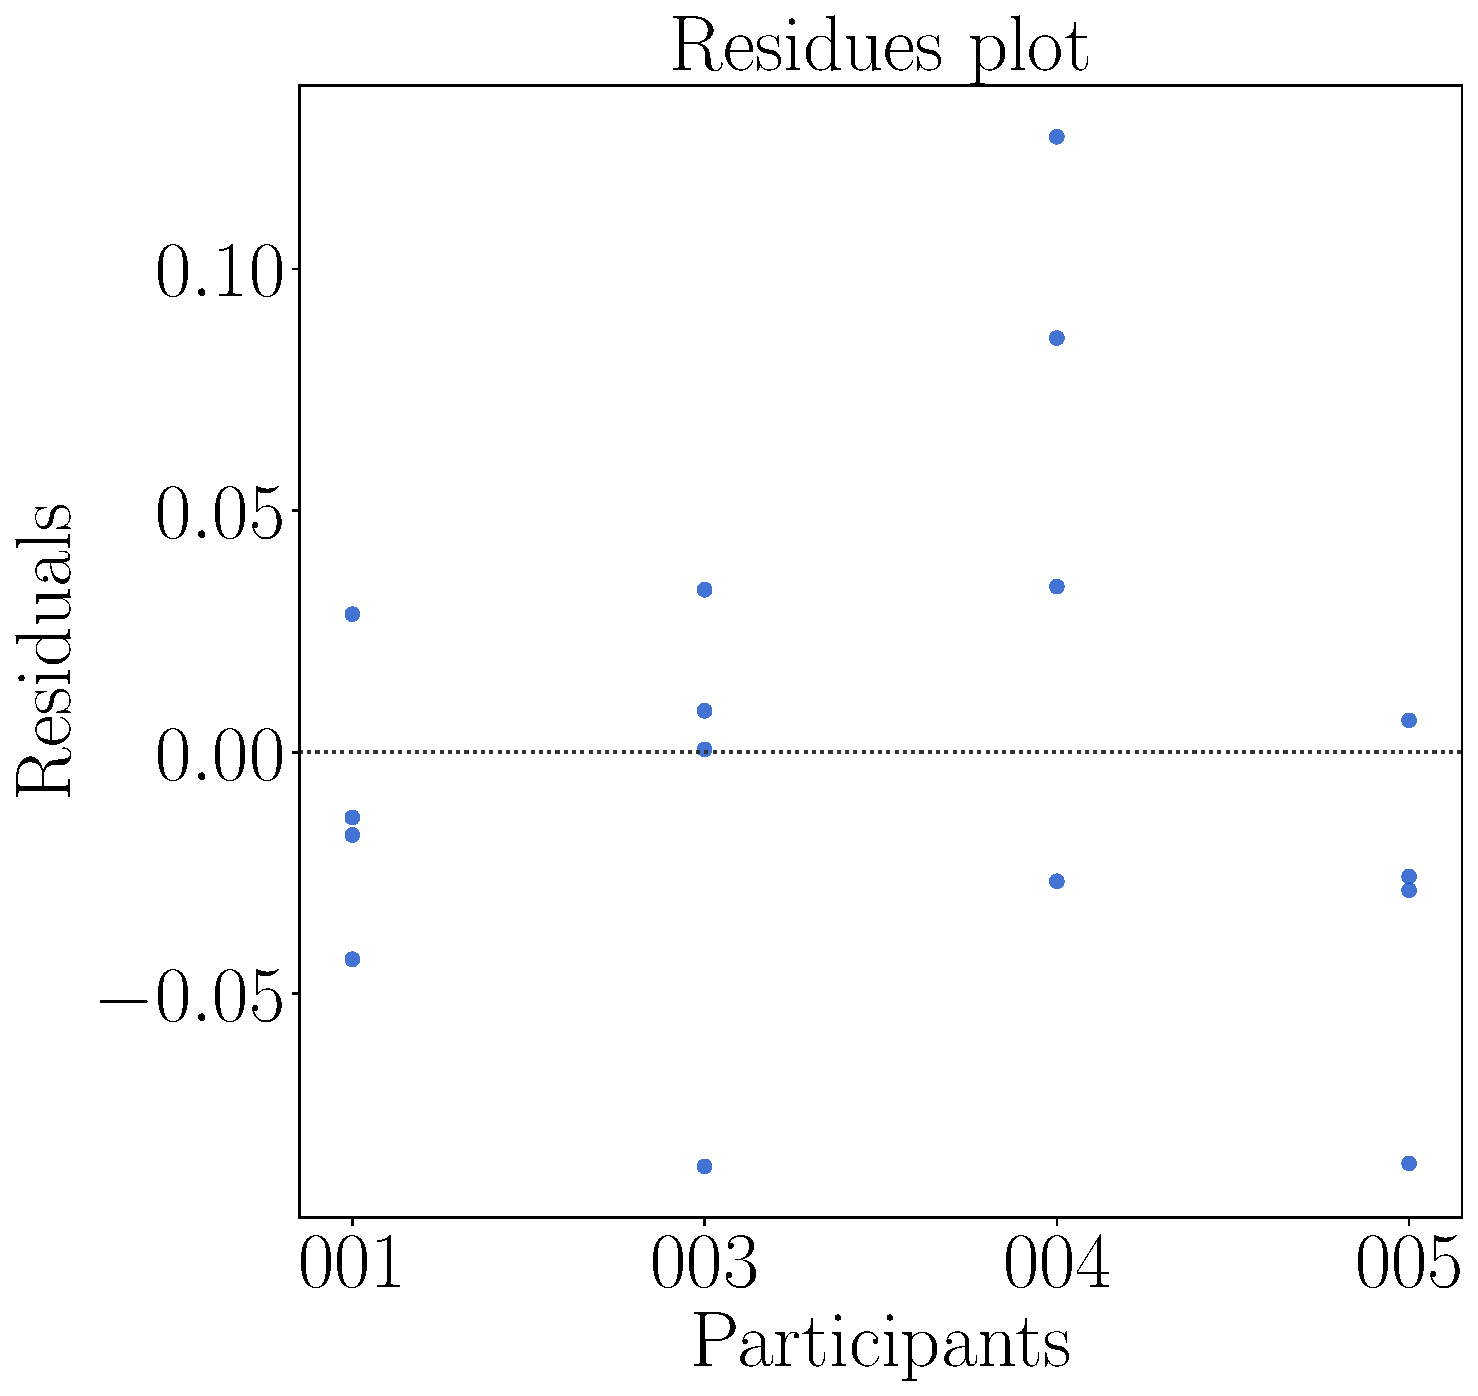
\includegraphics[width = \textwidth]{Resultados/Questionario/Figuras/pdf/residplot_questionnaire_sight.pdf}
%        \caption{Residual plot of the questionnaire score the sighted participants on each method.}
%        \label{fig:residplot_questionnaire_sight}
%    \end{minipage}
%\end{figure}
%
Table \ref{tab:lsd_questionnaire_blind_sight} presents the conclusion of 
A pairwise Fisher LSD test between all the guidance methods for both groups shows that the results are coincident between the two groups.

%\FloatBarrier

\begin{table*}[!thb]
    \caption{Anova p-value for the mental demand average on each method'}
    \label{tab:lsd_questionnaire_blind_sight}
    \begin{minipage}{1\textwidth}
        \subcaption{Blind participants.}
        
\centering
\begin{tabular}{rcllr}
\toprule
      \multicolumn{3}{c}{Method} &                          \multicolumn{2}{c}{Analysis} \\
\midrule
       Audio & $X$ & Haptic Belt &        $H_1 : \mu_{Audio} \ne \mu_{Haptic Belt}$ & ** \\
      Audio & $X$ & Virtual Cane &       $H_1 : \mu_{Audio} \ne \mu_{Virtual Cane}$ & ** \\
           Audio & $X$ & Mixture &                $H_0 : \mu_{Audio} = \mu_{Mixture}$ &  \\
Haptic Belt & $X$ & Virtual Cane & $H_1 : \mu_{Haptic Belt} \ne \mu_{Virtual Cane}$ & ** \\
     Haptic Belt & $X$ & Mixture &      $H_1 : \mu_{Haptic Belt} \ne \mu_{Mixture}$ & ** \\
    Virtual Cane & $X$ & Mixture &     $H_1 : \mu_{Virtual Cane} \ne \mu_{Mixture}$ & ** \\
\bottomrule
\end{tabular}

    \end{minipage}
    \begin{minipage}{1\textwidth}
        \subcaption{Sight participants.}
        
\centering
\begin{tabular}{rcllr}
\toprule
      \multicolumn{3}{c}{Method} &                          \multicolumn{2}{c}{Analysis} \\
\midrule
       Audio & $X$ & Haptic Belt &        $H_1 : \mu_{Audio} \ne \mu_{Haptic Belt}$ & ** \\
      Audio & $X$ & Virtual Cane &       $H_1 : \mu_{Audio} \ne \mu_{Virtual Cane}$ & ** \\
           Audio & $X$ & Mixture &                $H_0 : \mu_{Audio} = \mu_{Mixture}$ &  \\
Haptic Belt & $X$ & Virtual Cane & $H_1 : \mu_{Haptic Belt} \ne \mu_{Virtual Cane}$ & ** \\
     Haptic Belt & $X$ & Mixture &      $H_1 : \mu_{Haptic Belt} \ne \mu_{Mixture}$ & ** \\
    Virtual Cane & $X$ & Mixture &     $H_1 : \mu_{Virtual Cane} \ne \mu_{Mixture}$ & ** \\
\bottomrule
\end{tabular}

    \end{minipage}
\end{table*}

%\input{Resultados/Questionario/Tabelas/lsd_questionnaire.tex}

%The LSD Table \ref{tab:lsd_questionnaire_sight} repeat the same conclusion of the blind participants, that only the "Audio" and "Mixture" are statistically the same. But that does not mean that both groups had the same opinion from the rest of the methods. As shown in the Figure \ref{fig:boxplot_questionnaire_scene}, the average sighted user rather use the "Virtual Cane" then the "Haptic Belt", despite that distribution being wider, hence more varied, meaning that this is hardly a consense between the users.

%\FloatBarrier
%\subsection{Subjective data}
\subsubsection{NASA-TLX}
\label{subsubsec:results_nasa_tlx_2}

\paragraph*{Analysis of the mental demand scale}\mbox{}\\

Figures \ref{fig:boxplot_noBase_md_4_scene} and \ref{fig:boxplot_noBase_md_4_rounds} presents the box plot for both groups, organized by the methods and the rounds. The mental demand is systematically higher for sighted people, which is expected. However, while blind participants considered the audio method less demanding, sighted participants prefered to the virtual cane. For both groups, we observe a decrease in the mental demand.

\begin{figure}[!htb]
    \centering
    \includegraphics[width = 0.75\linewidth]{3 - Resultados/Figuras/boxplot_noBase_md_4_scene.pdf}
    \caption{Boxplot of the mental demand of the participants grouped by the methods.}
    \label{fig:boxplot_noBase_md_4_scene}
\end{figure}
\begin{figure}[!htb]
    \centering
    \includegraphics[width = 0.75\linewidth]{3 - Resultados/Figuras/boxplot_noBase_md_4_rounds.pdf}
    \caption{Boxplot of the mental demand of the participants grouped by the rounds.}
    \label{fig:boxplot_noBase_md_4_rounds}
\end{figure}

Table \ref{tab:blocanova_md_avg_two_way_blind_sight} brings the results of ANOVA. Unlike the blind participants, in the case of sighted ones, the p-value for the methods is below the threshold of 0.05, confirming it as a significant variable for the mental demand. In the case of the rounds, the data from both sighted and blind participants resulted in the exact p-value of 0.075, which is close to the traditional threshold of 0.05 but slightly higher. 

\begin{table}[!htb]
    \caption{Anova p-value for the mental demand average on each method'}
    \label{tab:blocanova_md_avg_two_way_blind_sight}
\begin{minipage}{0.45\linewidth}
    \subcaption{Blind participants}
    
\centering
\begin{tabular}{ll}
\toprule
          Source & P-Value \\
\midrule
    \    Methods &   0.170 \\
     \    Rounds &   0.075 \\
\    Interaction &   0.993 \\
\bottomrule
\end{tabular}

\end{minipage}%
\begin{minipage}{0.05\linewidth}
    \hfill
\end{minipage}%
\begin{minipage}{0.45\linewidth}
    \subcaption{Sight participants}
    
\centering
\begin{tabular}{ll}
\toprule
          Source & P-Value \\
\midrule
    \    Methods & 0.049** \\
     \    Rounds &   0.075 \\
\    Interaction &   0.990 \\
\bottomrule
\end{tabular}
    
\end{minipage}
\end{table}


%%%%%%%%%%%%%%%%%%%%%%%%%%%%%%%%%%%%%%%%%%%%%%%%%%%%%%%%%%%%%%%%%%%%%%%%%%%%
%%%%%%%%%%%%%%%%%%%%%%%%%%%%%%%%%%%%%%%%%%%%%%%%%%%%%%%%%%%%%%%%%%%%%%%%%%%%
%%%%%%%%%%%%%%%%%%%%%%%%%%%%%%%%%%%%%%%%%%%%%%%%%%%%%%%%%%%%%%%%%%%%%%%%%%%%
%%%%%%%%%%%%%%%%%%%%%%%%%%%%%%%%%%%%%%%%%%%%%%%%%%%%%%%%%%%%%%%%%%%%%%%%%%%%


\paragraph*{Analysis of the NASA-TLX score}\mbox{}\\

Figures \ref{fig:boxplot_noBase_nasa_4_scene} and \ref{fig:boxplot_noBase_nasa_4_rounds} present the boxplots of the NASA-TLX global score. Again, it is possible to see that sighted people usually give higher workload scores than blind ones. The influence of the round is approximately the same. However, the order of preference of the methods is different.

\begin{figure}[!htb]
    \centering
    \includegraphics[width = 0.75\linewidth]{3 - Resultados/Figuras/boxplot_noBase_nasa_4_scene.pdf}
    \caption{Boxplot of the NASA-TLX score of the participants grouped by the methods.}
    \label{fig:boxplot_noBase_nasa_4_scene}
\end{figure}
\begin{figure}[!htb]
    \centering
    \includegraphics[width = 0.75\linewidth]{3 - Resultados/Figuras/boxplot_noBase_nasa_4_rounds.pdf}
    \caption{Boxplot of the NASA-TLX score of the participants grouped by the rounds.}
    \label{fig:boxplot_noBase_nasa_4_rounds}
\end{figure}

The p-values for both groups are presented in Table \ref{tab:blocanova_nasa_avg_two_way_blind_sight}. It confirms the influence of the round for both sighted and blind people. In the case of the methods, the p-value of blind is lower than the threshold of 0.5, while that of sighted is slightly higher.

\begin{table}[!thb]
    \caption{Anova p-value for the NASA-TLX score on each method}
    \label{tab:blocanova_nasa_avg_two_way_blind_sight}
    \begin{minipage}{0.45\linewidth}
        \subcaption{Blind participants}
        
\centering
\begin{tabular}{ll}
\toprule
          Source & P-Value \\
\midrule
    \    Methods & 0.029** \\
     \    Rounds & 0.022** \\
\    Interaction &   0.814 \\
\bottomrule
\end{tabular}

    \end{minipage}%
    \begin{minipage}{0.05\linewidth}
        \hfill
    \end{minipage}%
    \begin{minipage}{0.45\linewidth}
        \subcaption{Sight participants}
        
\centering
\begin{tabular}{ll}
\toprule
          Source & P-Value \\
\midrule
    \    Methods &   0.086 \\
     \    Rounds & 0.034** \\
\    Interaction &   0.688 \\
\bottomrule
\end{tabular}
    
    \end{minipage}
\end{table}
\subsubsection{Adapted SAGAT}
\label{subsubsec:results_adapted_sagat_2}

Figures \ref{fig:boxplot_sagat_4_scene} and \ref{fig:boxplot_sagat_4_rounds} bring the boxplots. According to Figure \ref{fig:boxplot_sagat_4_scene}, both groups presented a higher situation awareness with ‘mixture’ and ‘haptic’. On the other hand, Figure \ref{fig:boxplot_sagat_4_rounds} confirms that the difference between the rounds is more significant for blind participants. 

\begin{figure}[!htb]
    \centering
    \includegraphics[width = 0.75\linewidth]{3 - Resultados//Figuras/boxplot_sagat_4_scene.pdf}
    \caption{Boxplot of the SAGAT score of the participants grouped by the methods.}
    \label{fig:boxplot_sagat_4_scene}
\end{figure}
\begin{figure}[!htb]
    \centering
    \includegraphics[width = 0.75\linewidth]{3 - Resultados//Figuras/boxplot_sagat_4_rounds.pdf}
    \caption{Boxplot of the SAGAT score of the participants grouped by the rounds.}
    \label{fig:boxplot_sagat_4_rounds}
\end{figure}

The variance of the residuals is not equal among the participants. Table \ref{tab:blocanova_sagat_avg_two_way_blind_sight} brings the p-value from ANOVA. While for the blind participants, the rounds are a significant factor and the methods are not, for the sighted participants the result is the opposite, showing a significant influence of the methods and not of the rounds.

\begin{table}[!htb]
    \caption{Anova p-value for the SAGAT score on each method}
    \label{tab:blocanova_sagat_avg_two_way_blind_sight}
\begin{minipage}{0.45\linewidth}
    \subcaption{Blind participants}
    
\centering
\begin{tabular}{ll}
\toprule
          Source & P-Value \\
\midrule
    \    Methods &   0.277 \\
     \    Rounds & 0.002** \\
\    Interaction &   0.834 \\
\bottomrule
\end{tabular}

\end{minipage}%
\begin{minipage}{0.05\linewidth}
    \hfill
\end{minipage}%
\begin{minipage}{0.45\linewidth}
    \subcaption{Sight participants}
    
\centering
\begin{tabular}{ll}
\toprule
          Source & P-Value \\
\midrule
    \    Methods & 0.035** \\
     \    Rounds &   0.095 \\
\    Interaction &   0.578 \\
\bottomrule
\end{tabular}
    
\end{minipage}
\end{table}
\subsubsection{Guidance method's questionnaire.}
\label{subsubsec:results_questionnaires_2}

The Figure \ref{fig:boxplot_questionnaire_scene} presents the box plot with the distribution of the scores. It is possible to see that there is some similarity between the two groups, except for the virtual cane method, which has a broader distribution for the sighted users. Also, it seems that the audio and mixture have similar acceptance for sighted and blind users.

\begin{figure}[!htb]
    \centering
    \includegraphics[width = 0.75\linewidth]{3 - Resultados/Figuras/boxplot_questionnaire_scene.pdf}
    \caption{Boxplot of the questionaire score of the the participants grouped by the methods.}
    \label{fig:boxplot_questionnaire_scene}
\end{figure}

The result of ANOVA is presented in Table \ref{tab:blocanova_questionnaire_blind_sight} and indicates that the method is an effective variable for the sighted participants, as it is for the blind ones.

\begin{table}[!htb]
    \caption{Anova p-value for the questionnaire score on each method}
    \label{tab:blocanova_questionnaire_blind_sight}
\begin{minipage}{0.45\linewidth}
    \subcaption{Blind participants.}
    
\centering
\begin{tabular}{ll}
\toprule
Source & P-Value \\
\midrule
Method & 0.001** \\
\bottomrule
\end{tabular}

\end{minipage}%
\begin{minipage}{0.05\linewidth}
\end{minipage}%
\begin{minipage}{0.45\linewidth}
    \subcaption{Sight participants.}
    
\centering
\begin{tabular}{ll}
\toprule
Source & P-Value \\
\midrule
Method & 0.016** \\
\bottomrule
\end{tabular}

\end{minipage}
\end{table}

Table \ref{tab:lsd_questionnaire_blind_sight} presents the conclusion of 
A pairwise Fisher LSD test between all the guidance methods for both groups shows that the results are coincident between the two groups.

%\FloatBarrier

\begin{table*}[!thb]
    \caption{Anova p-value for the mental demand average on each method'}
    \label{tab:lsd_questionnaire_blind_sight}
    \begin{minipage}{1\textwidth}
        \subcaption{Blind participants.}
        
\centering
\begin{tabular}{rcllr}
\toprule
      \multicolumn{3}{c}{Method} &                          \multicolumn{2}{c}{Analysis} \\
\midrule
       Audio & $X$ & Haptic Belt &        $H_1 : \mu_{Audio} \ne \mu_{Haptic Belt}$ & ** \\
      Audio & $X$ & Virtual Cane &       $H_1 : \mu_{Audio} \ne \mu_{Virtual Cane}$ & ** \\
           Audio & $X$ & Mixture &                $H_0 : \mu_{Audio} = \mu_{Mixture}$ &  \\
Haptic Belt & $X$ & Virtual Cane & $H_1 : \mu_{Haptic Belt} \ne \mu_{Virtual Cane}$ & ** \\
     Haptic Belt & $X$ & Mixture &      $H_1 : \mu_{Haptic Belt} \ne \mu_{Mixture}$ & ** \\
    Virtual Cane & $X$ & Mixture &     $H_1 : \mu_{Virtual Cane} \ne \mu_{Mixture}$ & ** \\
\bottomrule
\end{tabular}

    \end{minipage}
    \begin{minipage}{1\textwidth}
        \subcaption{Sight participants.}
        
\centering
\begin{tabular}{rcllr}
\toprule
      \multicolumn{3}{c}{Method} &                          \multicolumn{2}{c}{Analysis} \\
\midrule
       Audio & $X$ & Haptic Belt &        $H_1 : \mu_{Audio} \ne \mu_{Haptic Belt}$ & ** \\
      Audio & $X$ & Virtual Cane &       $H_1 : \mu_{Audio} \ne \mu_{Virtual Cane}$ & ** \\
           Audio & $X$ & Mixture &                $H_0 : \mu_{Audio} = \mu_{Mixture}$ &  \\
Haptic Belt & $X$ & Virtual Cane & $H_1 : \mu_{Haptic Belt} \ne \mu_{Virtual Cane}$ & ** \\
     Haptic Belt & $X$ & Mixture &      $H_1 : \mu_{Haptic Belt} \ne \mu_{Mixture}$ & ** \\
    Virtual Cane & $X$ & Mixture &     $H_1 : \mu_{Virtual Cane} \ne \mu_{Mixture}$ & ** \\
\bottomrule
\end{tabular}

    \end{minipage}
\end{table*}


%\subsection{Physiological data}

\subsubsection{Electrocardiogram (ECG) data}
\label{subsubsec:results_ecg_2}

\paragraph*{Analysis of the heartbeat frequency (BPM)}\mbox{}\\

If the variation between the First and the Return round is positive, it means that the user had an increase on his/her mental workload and vice-versa. Comparing the two groups, the audio method is associated with a slightly lower heart rate for blind people, but the opposite happens for sighted participants. Moreover, data from blind participants have a significant variance. This significant variance can also be observed in the boxplot of Figures \ref{fig:boxplot_ecg_bpm_4_scene} and \ref{fig:boxplot_ecg_bpm_4_rounds}. 

\begin{figure}[!htb]
    \centering
    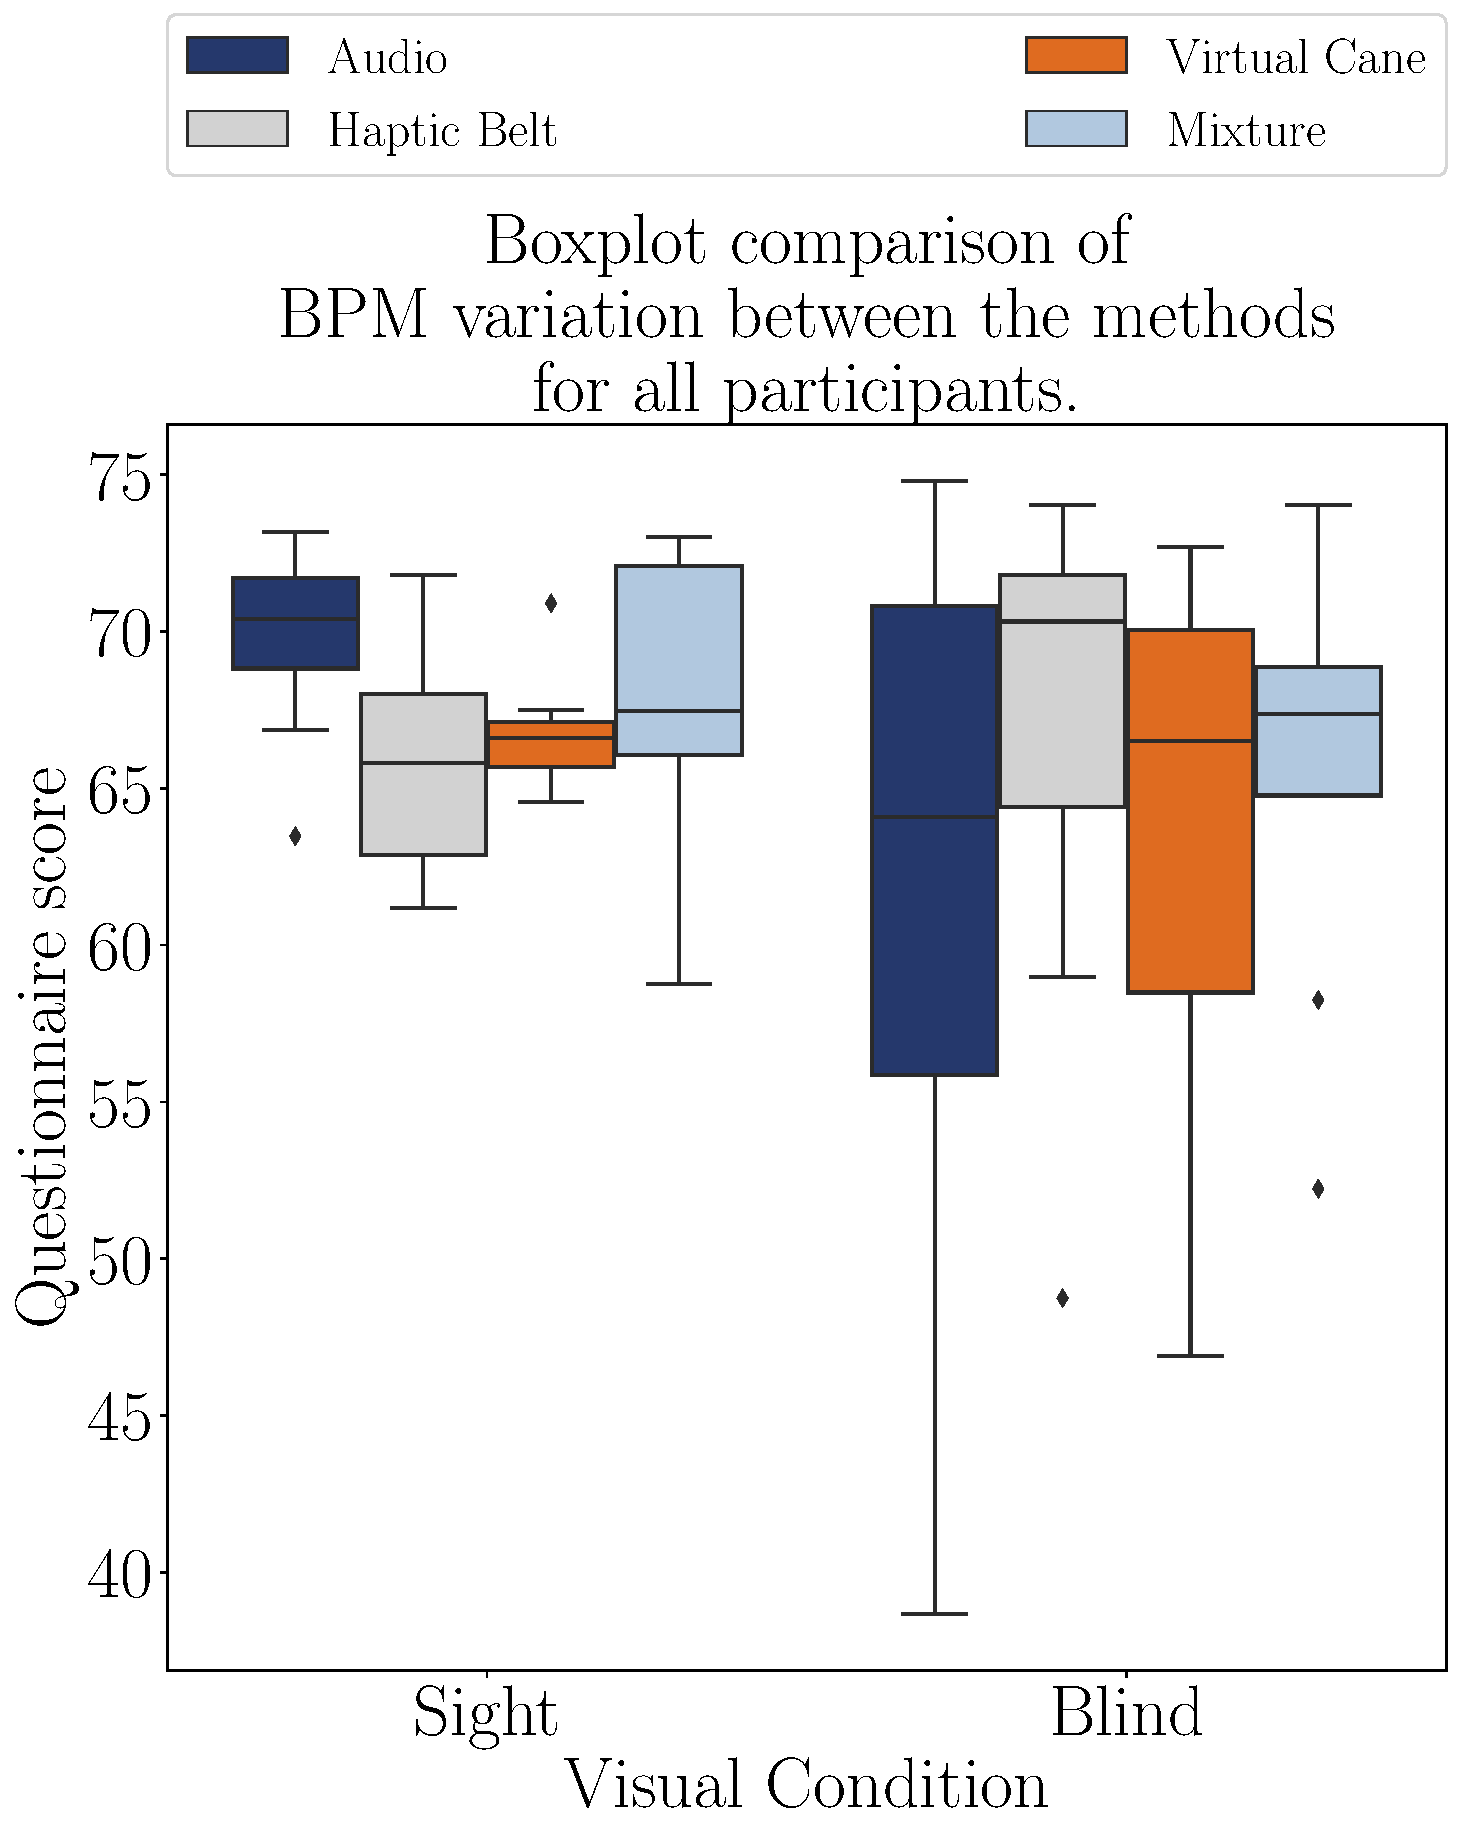
\includegraphics[width = 0.75\linewidth]{3 - Resultados/Figuras/boxplot_ecg_bpm_4_scene.pdf}
    \caption{Boxplot of the average BPM of the participants grouped by the methods.}
    \label{fig:boxplot_ecg_bpm_4_scene}
\end{figure}
\begin{figure}[!htb]
    \centering
    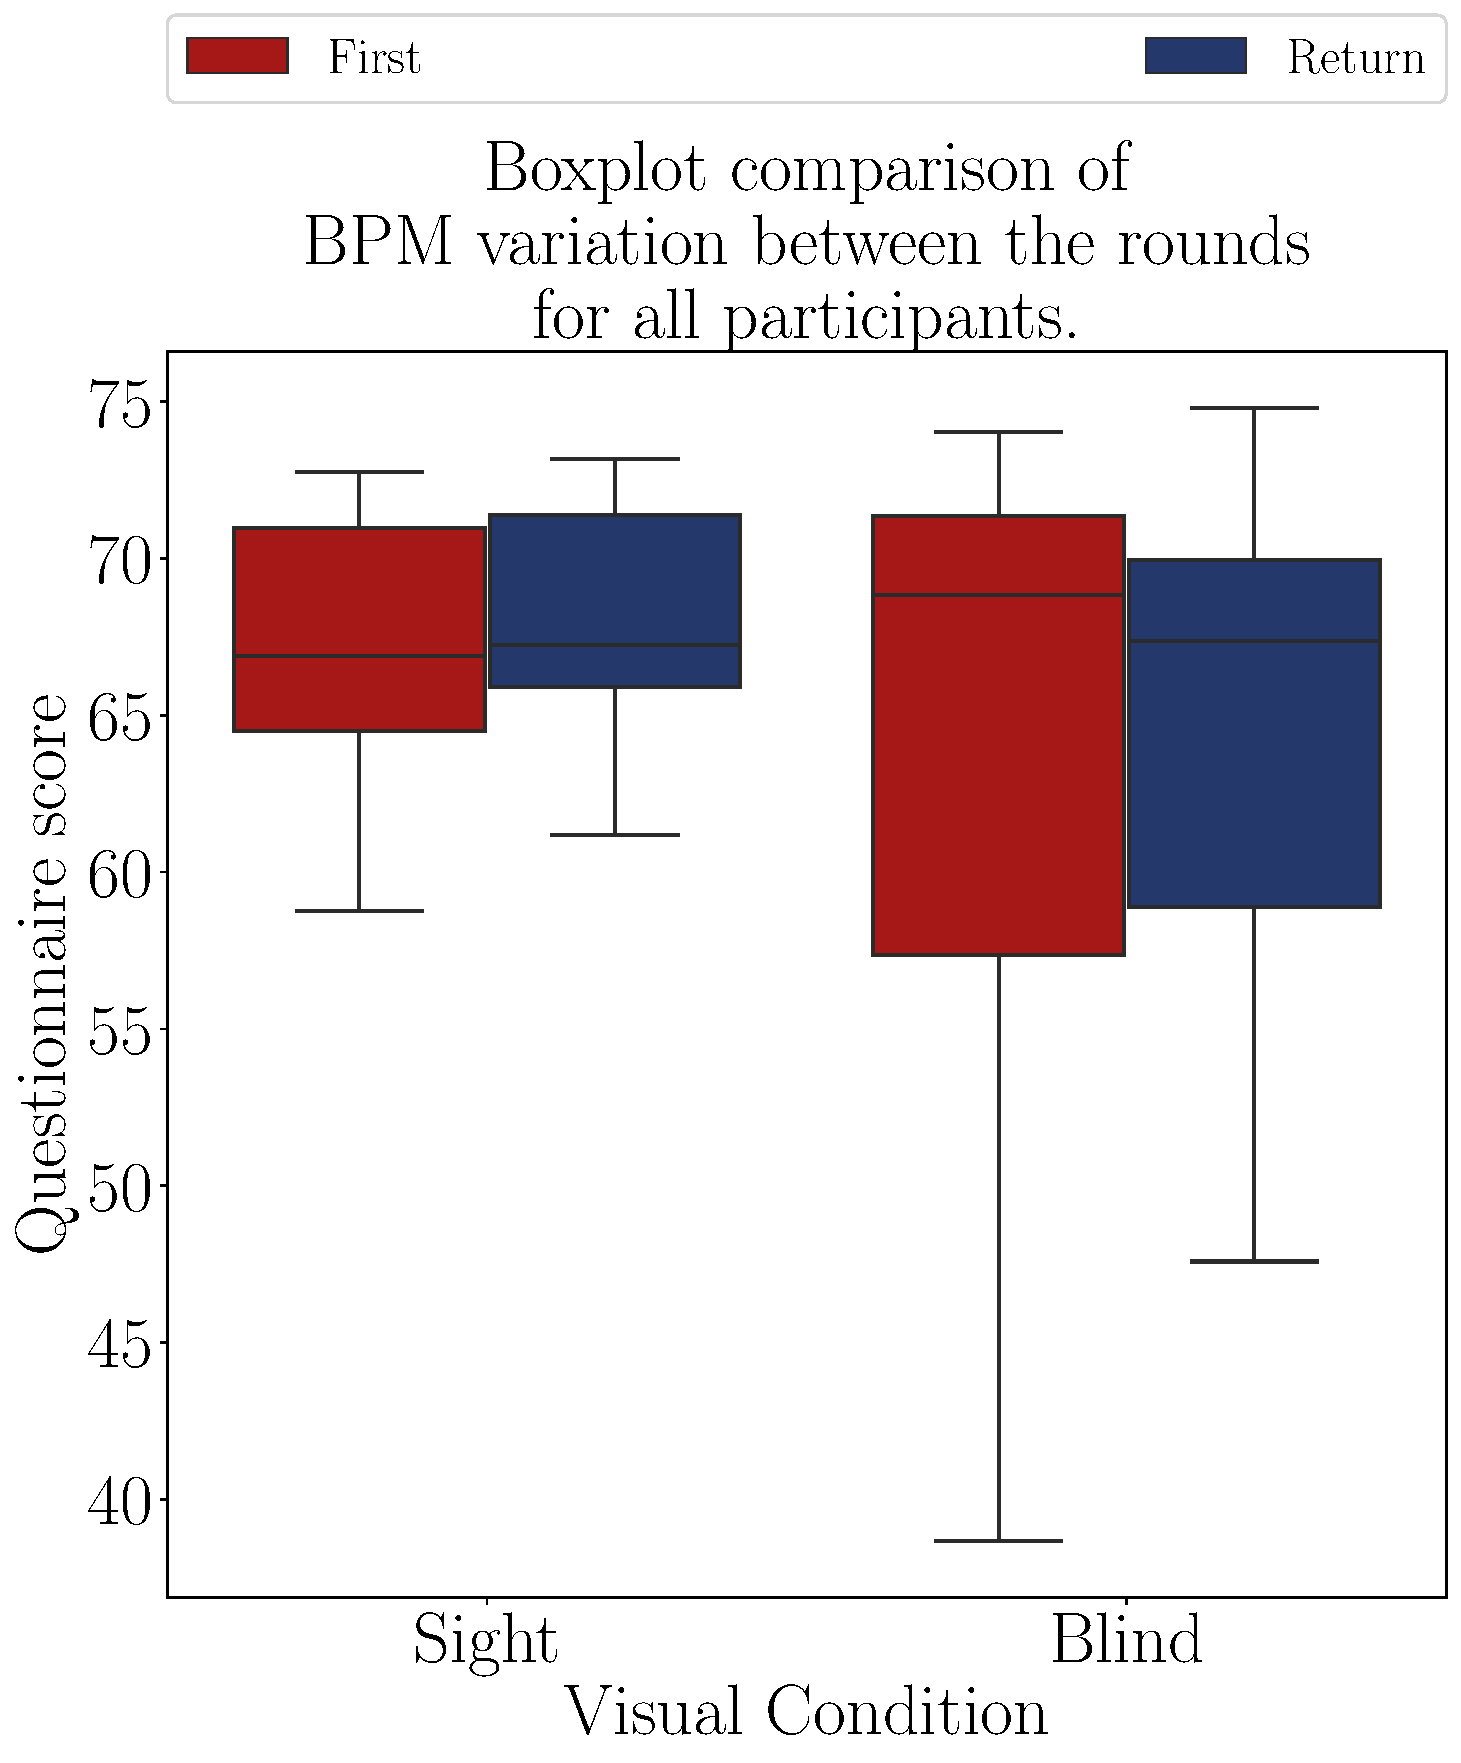
\includegraphics[width = 0.75\linewidth]{3 - Resultados/Figuras/boxplot_ecg_bpm_4_rounds.pdf}
    \caption{Boxplot of the average BPM of the participants grouped by the rounds.}
    \label{fig:boxplot_ecg_bpm_4_rounds}
\end{figure}

Table \ref{tab:blocanova_bpm_two_way_blind_sight} brings the results from ANOVA, which are similar for both sighted and blind participants.

\begin{table}[!htb]
    \caption{Anova p-value for the BPM on each method.}
    \label{tab:blocanova_bpm_two_way_blind_sight}
\begin{minipage}{0.45\linewidth}
    \subcaption{Blind participants}
    \input{3 - Resultados/Tabelas/blocanova_bpm_two_way_blindsemBegin.tex}
\end{minipage}%
\begin{minipage}{0.05\linewidth}
    \hfill
\end{minipage}%
\begin{minipage}{0.45\linewidth}
    \subcaption{Sight participants}
    \input{3 - Resultados/Tabelas/blocanova_bpm_two_way_sightsemBegin.tex}
\end{minipage}
\end{table}


%%%%%%%%%%%%%%%%%%%%%%%%%%%%%%%%%%%%%%%%%%%%%%%%%%%%%%%%%%%%%%%%%%%%%%%%%%%%
%%%%%%%%%%%%%%%%%%%%%%%%%%%%%%%%%%%%%%%%%%%%%%%%%%%%%%%%%%%%%%%%%%%%%%%%%%%%
%%%%%%%%%%%%%%%%%%%%%%%%%%%%%%%%%%%%%%%%%%%%%%%%%%%%%%%%%%%%%%%%%%%%%%%%%%%%
%%%%%%%%%%%%%%%%%%%%%%%%%%%%%%%%%%%%%%%%%%%%%%%%%%%%%%%%%%%%%%%%%%%%%%%%%%%%

\paragraph*{Analysis of the heartbeat variance (SDNN)}\mbox{}\\

Figures \ref{fig:boxplot_ecg_sdnn_4_scene} and \ref{fig:boxplot_ecg_sdnn_4_rounds} shows the boxplots for both groups. Both pictures show that the SDNN of the sighted users was higher than that of the blind users, indicating that sighted users had a lower mental workload than the blind users.

\begin{figure}[!htb]
    \centering
    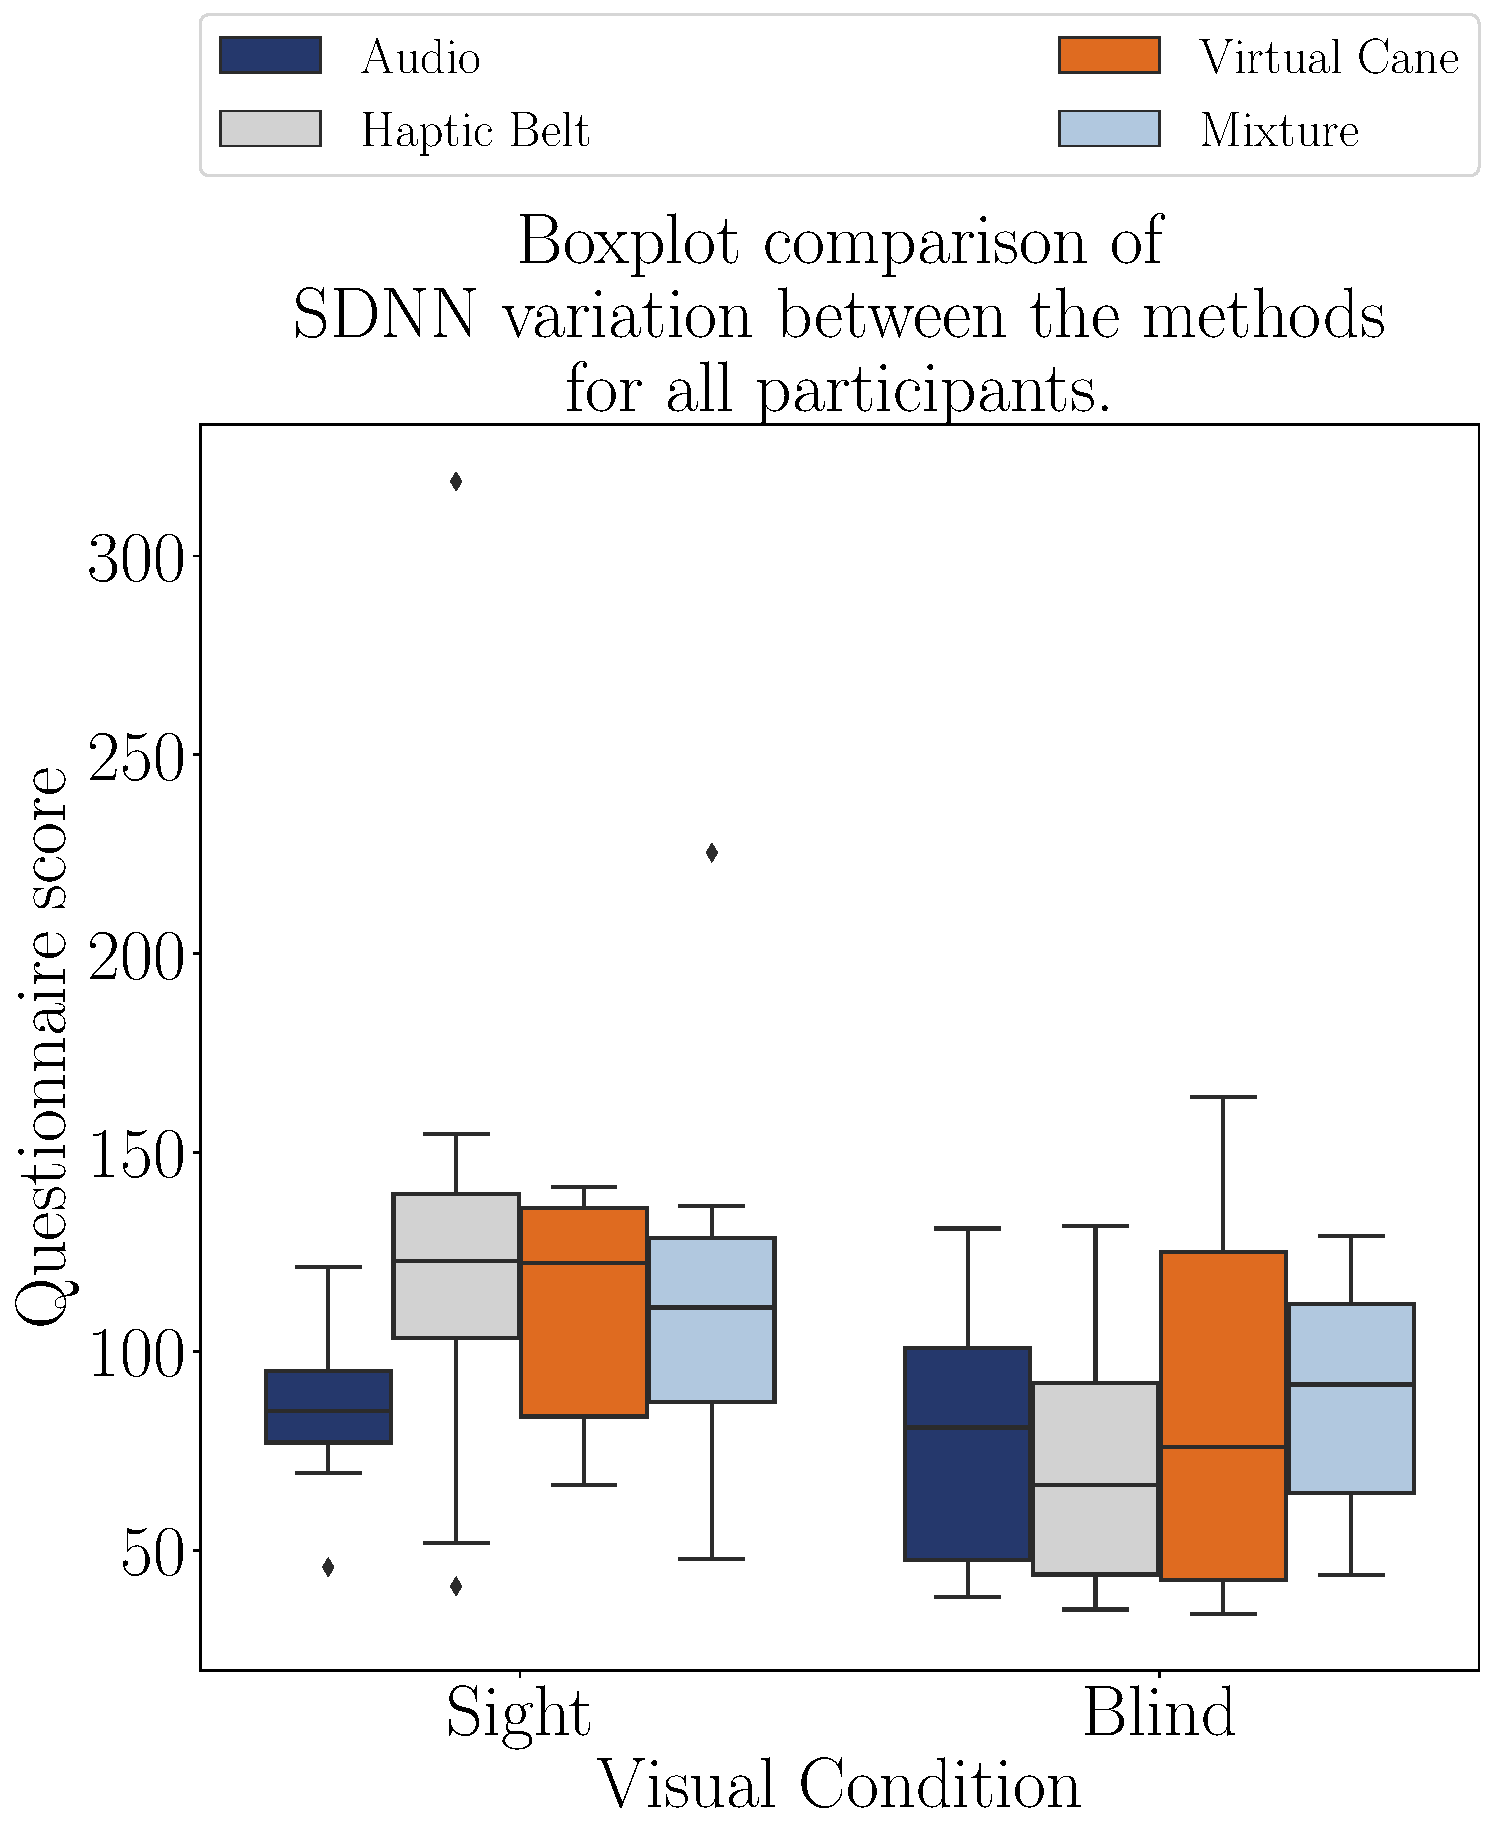
\includegraphics[width = 0.75\linewidth]{3 - Resultados/Figuras/boxplot_ecg_sdnn_4_scene.pdf}
    \caption{Boxplot of the average SDNN of the participants grouped by the methods.}
    \label{fig:boxplot_ecg_sdnn_4_scene}
\end{figure}
\begin{figure}[!htb]
    \centering
    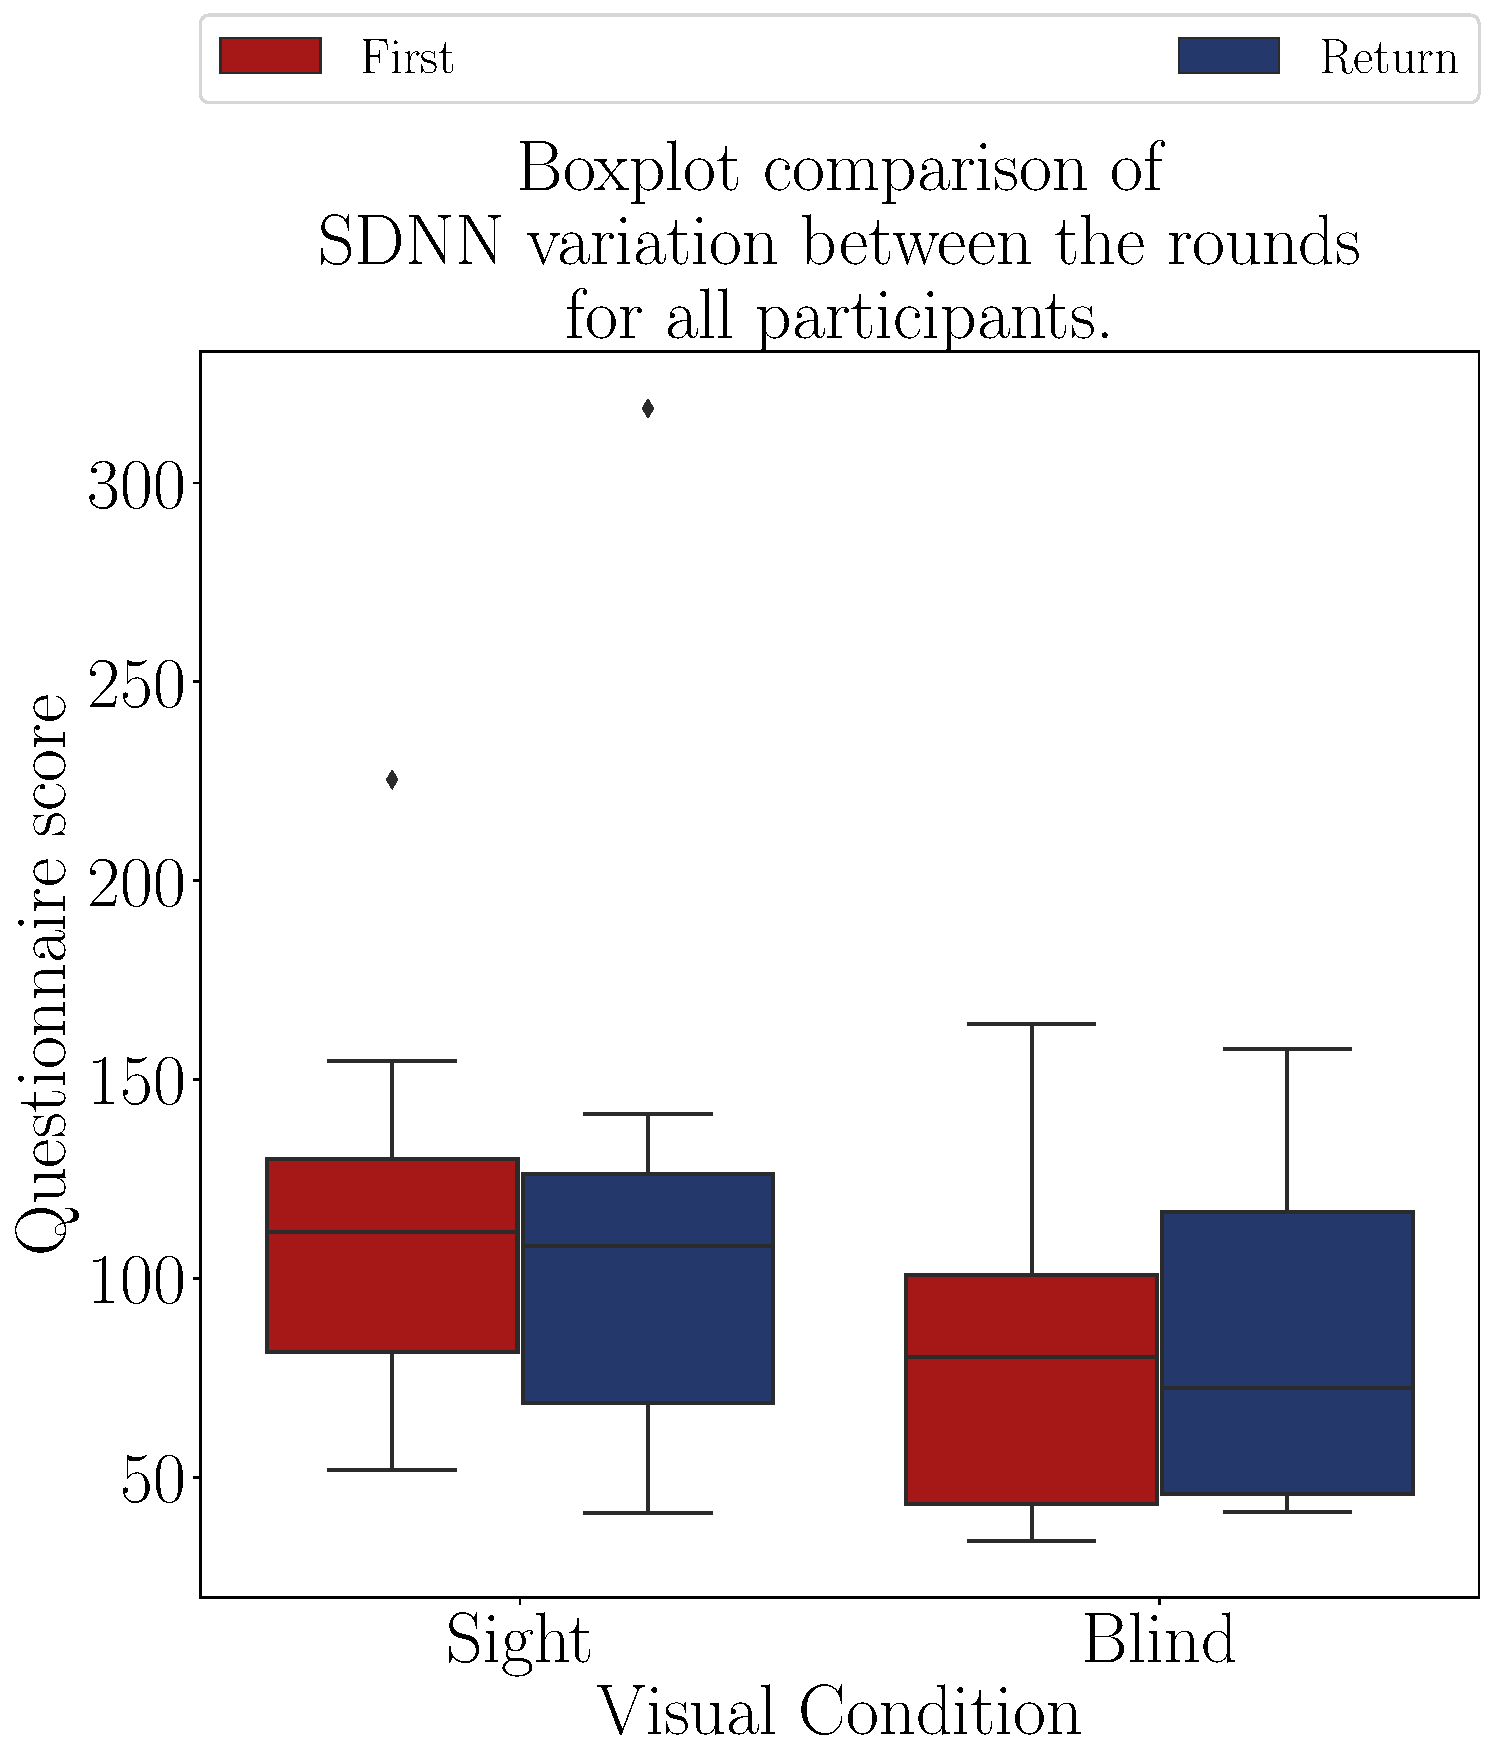
\includegraphics[width = 0.75\linewidth]{3 - Resultados/Figuras/boxplot_ecg_sdnn_4_rounds.pdf}
    \caption{Boxplot of the average SDNN of the participants grouped by the rounds.}
    \label{fig:boxplot_ecg_sdnn_4_rounds}
\end{figure}
 
Table \ref{tab:blocanova_sdnn_two_way_blind_sight} shows the ANOVA test p-values. For both groups, none of the factors have a significant influence on the SDNN value.

\begin{table}[!htb]
    \caption{Anova p-value for the average SDNN on each method.'}
    \label{tab:blocanova_sdnn_two_way_blind_sight}
\begin{minipage}{0.45\linewidth}
    \subcaption{Blind participants}
    \input{3 - Resultados/Tabelas/blocanova_sdnn_two_way_blindsemBegin.tex}
\end{minipage}%
\begin{minipage}{0.05\linewidth}
    \hfill
\end{minipage}%
\begin{minipage}{0.45\linewidth}
    \subcaption{Sight participants}
    \input{3 - Resultados/Tabelas/blocanova_sdnn_two_way_sightsemBegin.tex}
\end{minipage}
\end{table}
\subsubsection{Galvanic skin response and temperature data;}
\label{subsubsec:results_gsr_temp_2}

If the variation between the round and the Baseline is positive, it means that the user had an increase on his/her Mental Workload or stress. While the GSR varied for the blind participants, increasing for methods with vibration, the same does not happen for sighted participants. Also, the variance of GSR data for blind participants is significantly higher than that of sighted ones. The same conclusion can be drawn from the boxplots in Figures \ref{fig:boxplot_ecg_sdnn_4_scene} and \ref{fig:boxplot_ecg_sdnn_4_rounds}. 

\begin{figure}[!htb]
    \centering
    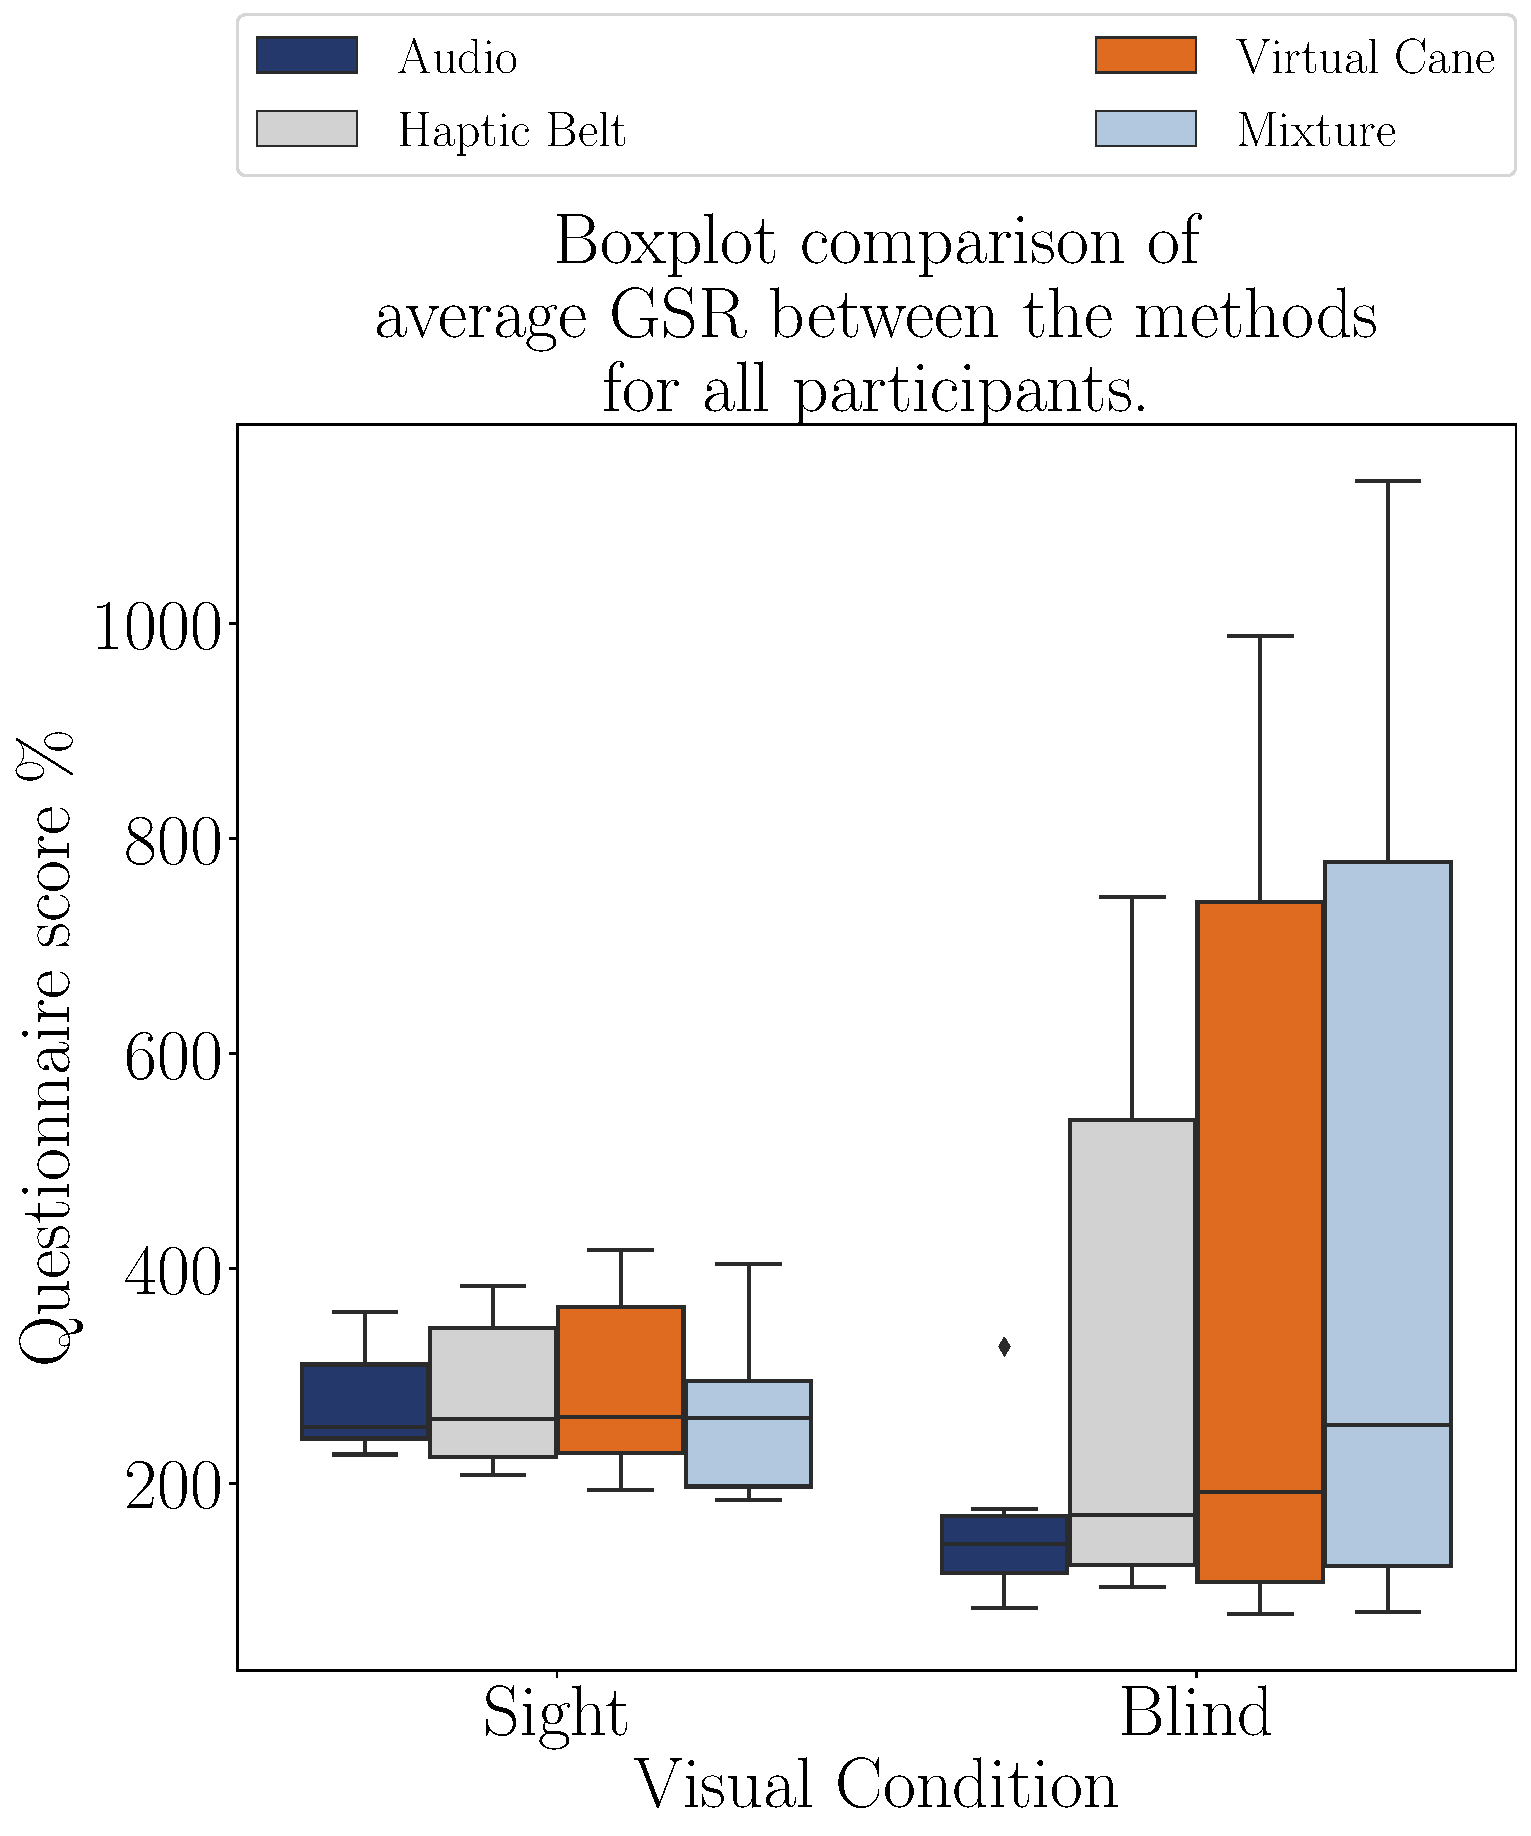
\includegraphics[width = 0.75\linewidth]{3 - Resultados/Figuras/boxplot_gsr_avg_4_scene.pdf}
    \caption{Boxplot of the average GSR of the participants grouped by method.}
    \label{fig:boxplot_gsr_avg_4_scene}
\end{figure}
\begin{figure}[!htb]
    \centering
    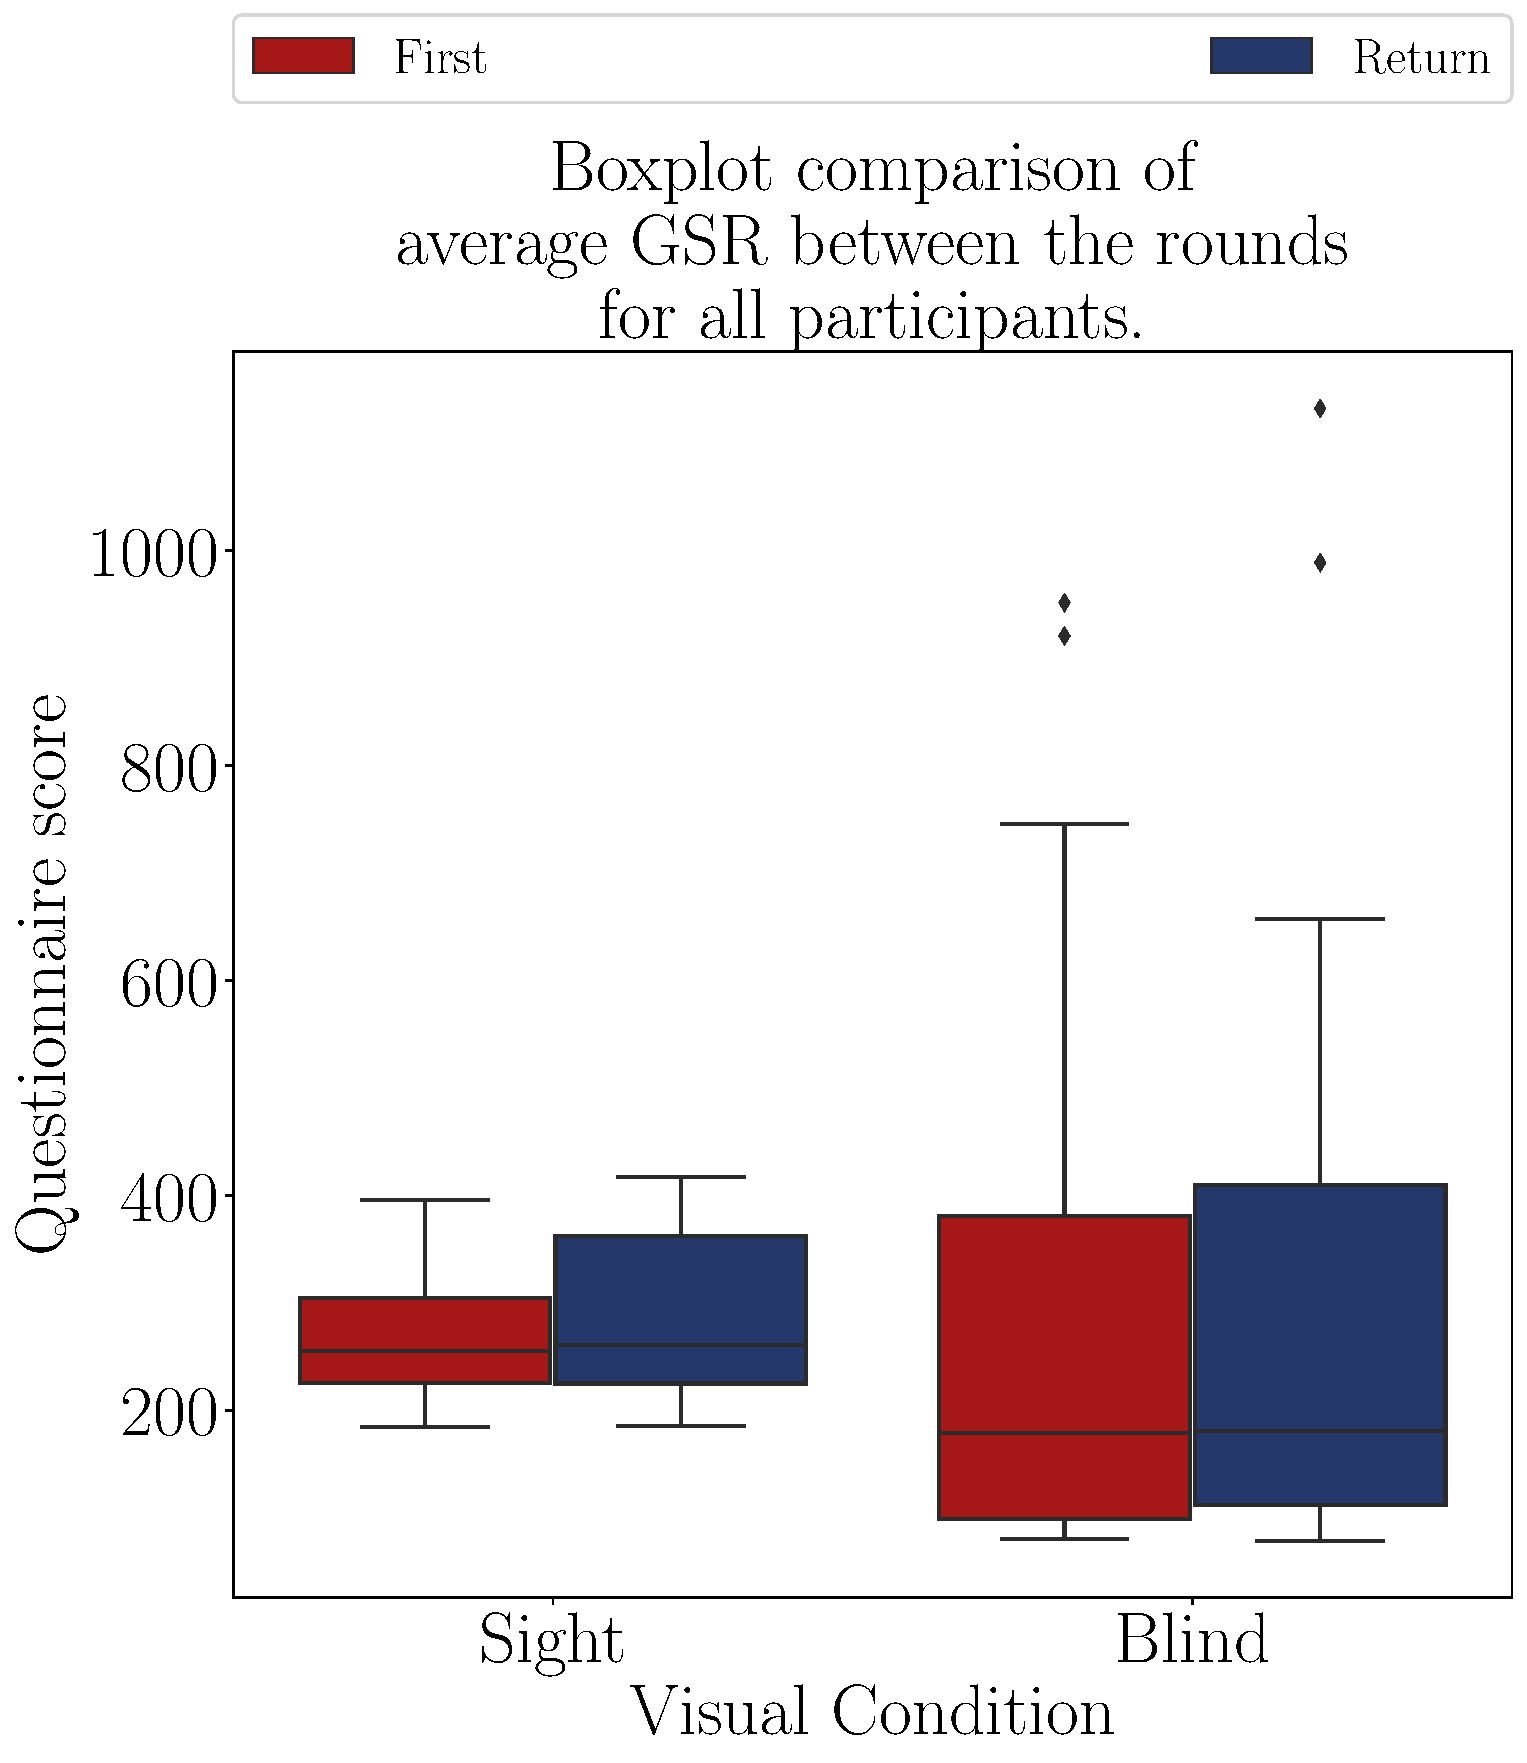
\includegraphics[width = 0.75\linewidth]{3 - Resultados/Figuras/boxplot_gsr_avg_4_rounds.pdf}
    \caption{Boxplot of the average GSR of the participants grouped by round.}
    \label{fig:boxplot_gsr_avg_4_rounds}
\end{figure}

The results from ANOVA are presented in Table \ref{tab:blocanova_gsr_two_way_blind_sight}. In the case of blind participants, the p-value for the method is just slightly over the threshold, indicating a possible influence of the method. The same does not happen with sighted participants, where the p-value of the method factor is the highest and well above the 0.05 threshold.

\begin{table}[!htb]
    \caption{Anova p-value for the skin conductance average on each method}
    \label{tab:blocanova_gsr_two_way_blind_sight}
\begin{minipage}{0.45\linewidth}
    \subcaption{Blind participants}
    \input{3 - Resultados/Tabelas/blocanova_gsr_two_way_blindsemBegin.tex}
\end{minipage}%
\begin{minipage}{0.05\linewidth}
    \hfill
\end{minipage}%
\begin{minipage}{0.45\linewidth}
    \subcaption{Sight participants}
    \input{3 - Resultados/Tabelas/blocanova_gsr_two_way_sightsemBegin.tex}
\end{minipage}
\end{table}

%\subsubsection*{Final Remarks}
%
%The comparison between the results from the blind participants and the sighted participants %showed that there are significant differences in the evaluation performed by each group.
%
%The sighted users evaluated the mental demand and other dimensions of NASA-TLX higher than %blind ones. Also, blind participants were more familiar with audio methods and therefore %gave a lower score to its mental demand. In the case of sighted participants, the method %that received the lowest score was the virtual cane. 
%
%The adapted SAGAT questionnaire showed a more significant influence of the round factor for %blind participants, which significantly improved their situation awareness on the return %round. In the case of sighted users, the difference between the rounds was not so striking. %Also, the score achieved by sighted participants was lower than that of blind users, which %was expected.
%
%Another difference is that, for blind participants, it was possible to observe a difference %between the methods that use vibration and those that do not. This difference was not clear %for sighted participants. 
%
%Besides these results, the sighted participants also gave feedback about the experiment. They felt considerably insecure when walking, even when hand-guided by another person. On the other hand, blind participants were already used to bumping their bodies when exploring new spaces. The sighted participants did not want that to happen and approached the furniture with caution. Similar to the blind participants, they also noticed the lack of precision of the haptic devices, but they did rely on them to navigate.